% Quickly access the figures.
\newcommand{\missionalphabetnode}[2]{{\includegraphics[height=#2]{figures/mission-grammars-alphabet/#1.png}}}
\newcommand{\missioninstruction}[1]{{\begin{minipage}{.3\textwidth}\includegraphics[width=35mm]{figures/mission-grammars-ins-rep/#1.png}\end{minipage}}}

\chapter{研究方法}
\label{cha:methodology}

本論文中,我們仍保持 Joris Dormans~\cite{dormans2010adventures}~\cite{dormans2012engineering} 與 Antonios Liapis~\cite{liapis2013generating} 為求遊戲設計過程抽象化與高階化的訴求。將「Mission/Space 框架」與「Multi-segment 演化」兩種關卡生成方法結合並予以改良,保留了前者追求的遊戲進程之順序性,後者帶來穩定且多樣化的遊戲內容,希冀藉此提升整體遊戲體驗、相輔相成。

圖~\ref{fig:system-framework} 為系統的整體流程。圖~\ref{fig:system-framework} a,遊戲設計師能夠透過宏觀的觀點來構築遊戲體驗流,將遊玩特徵拆分成多項規則,利用生成語法及改寫系統生成出任務圖 (mission graph)。圖~\ref{fig:system-framework} b-c,依照任務圖中對應的終端節點 (terminal nodes) 轉換為事先建構完成的房間容器 (volume),並得到尚未包含遊戲物件的遊戲地圖。圖~\ref{fig:system-framework} d-e,針對動作冒險遊戲我們提出了數項評估遊戲性的適應性函數 (fitness functions),藉由基因演算法演化房間容器的流程,令各房間遵守適應性函數的限制,以得到符合訴求的最適解。

\begin{figure}[!htb]
  \begin{center}
    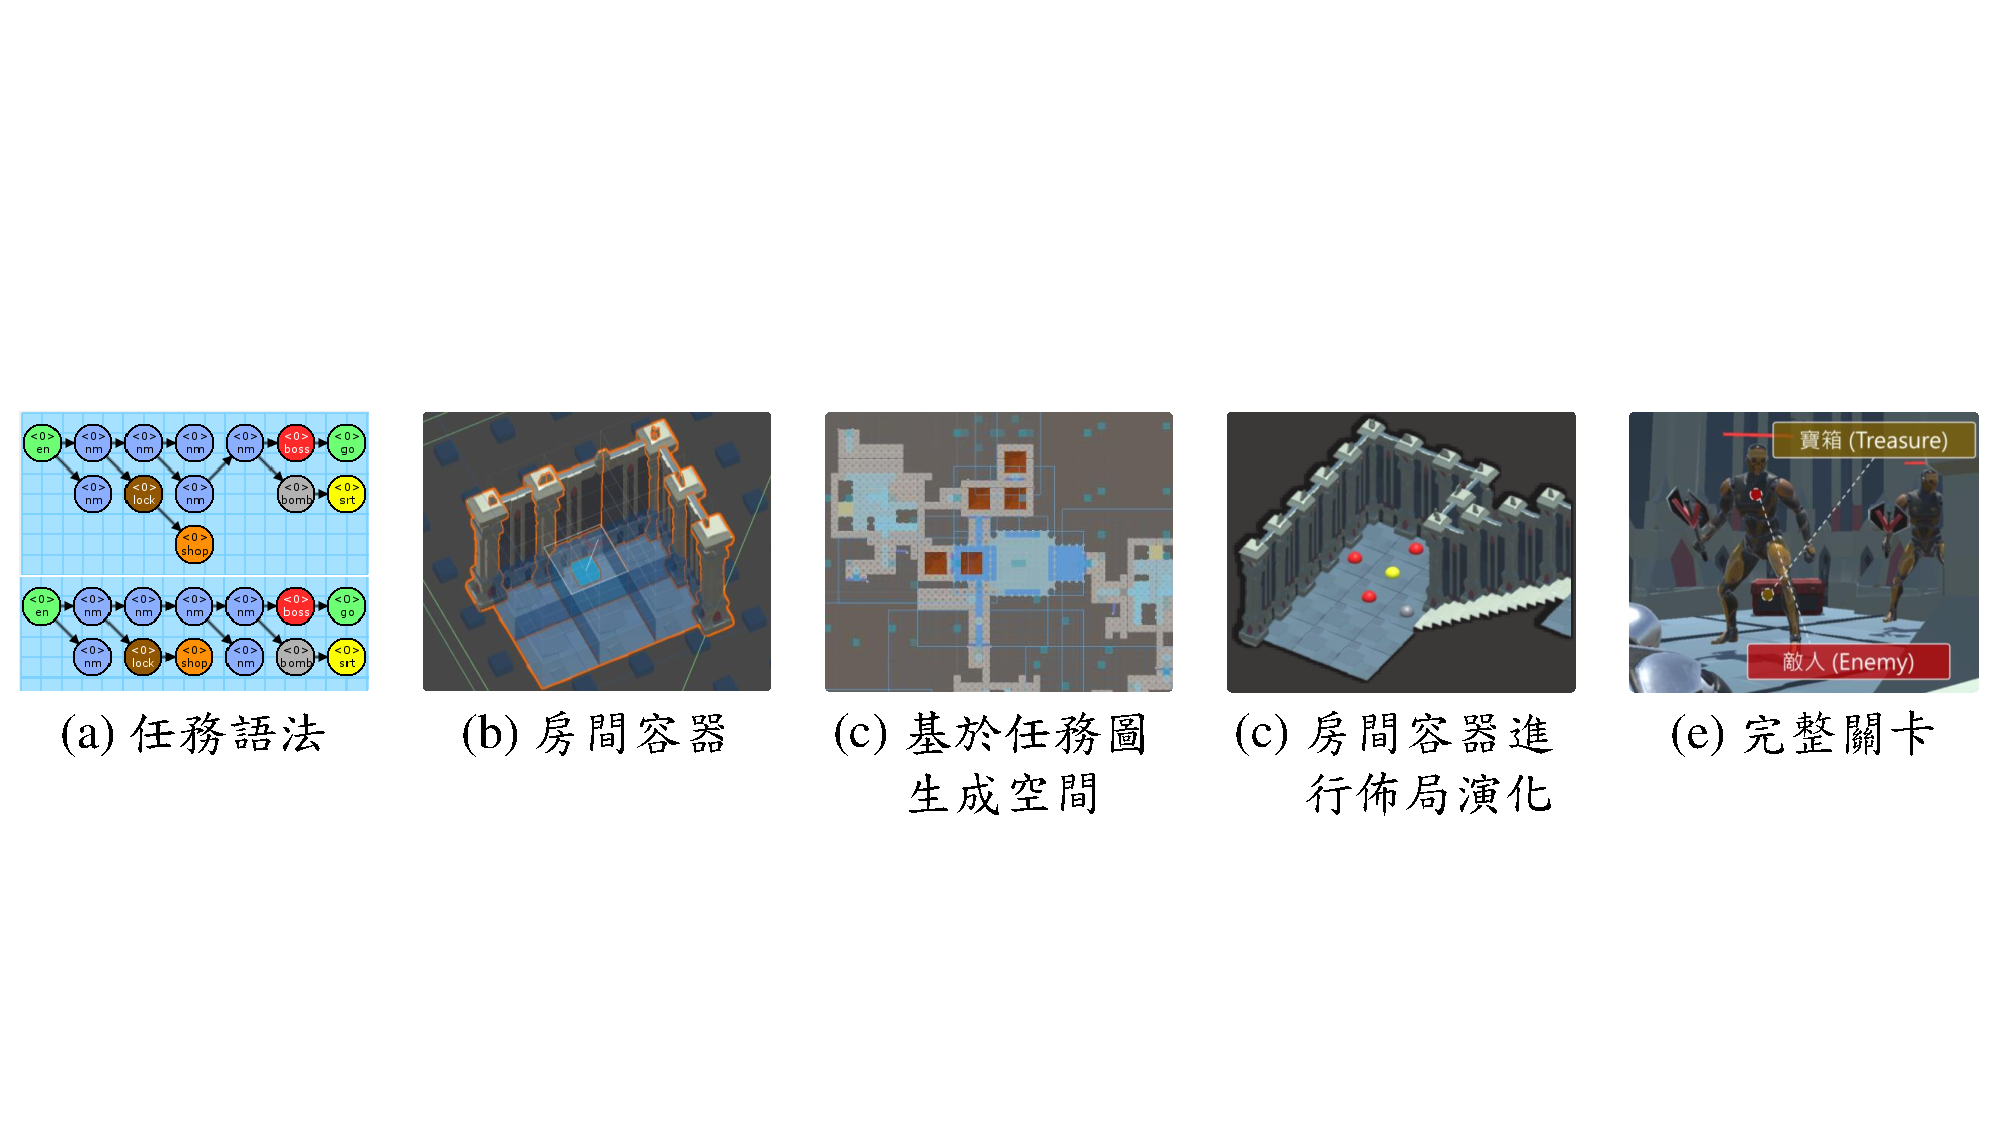
\includegraphics[width=1.0\textwidth]{figures/system-framework.pdf}
    \caption{本論文提出系統之流程} 
    \label{fig:system-framework}
  \end{center}
\end{figure}

\section{任務語法}
\label{sec:method-missiongrammars}

我們基於 Joris Dormans 提出之 Mission Grammars 概念,進行實作與改良出\textit{Dungeon Generator} 工具,見圖~\ref{fig:dungeon-generator}。遊戲設計師能夠藉由\textit{Dungeon Generator} 工具進行任務語法的建置,並執行改寫系統以輸出任務圖,進一步利用任務圖產出遊戲關卡空間。

在任務語法的設計階段,我們參考遊戲\textit{The binding of Isaac} 的關卡地圖,分析其遊戲進程結構,構想期望的任務圖並將觀察其遊玩特徵,接著拆分成任務語法規則使用改寫規則產生出近似結構的任務圖。

\begin{figure}[!htb]
  \begin{center}
    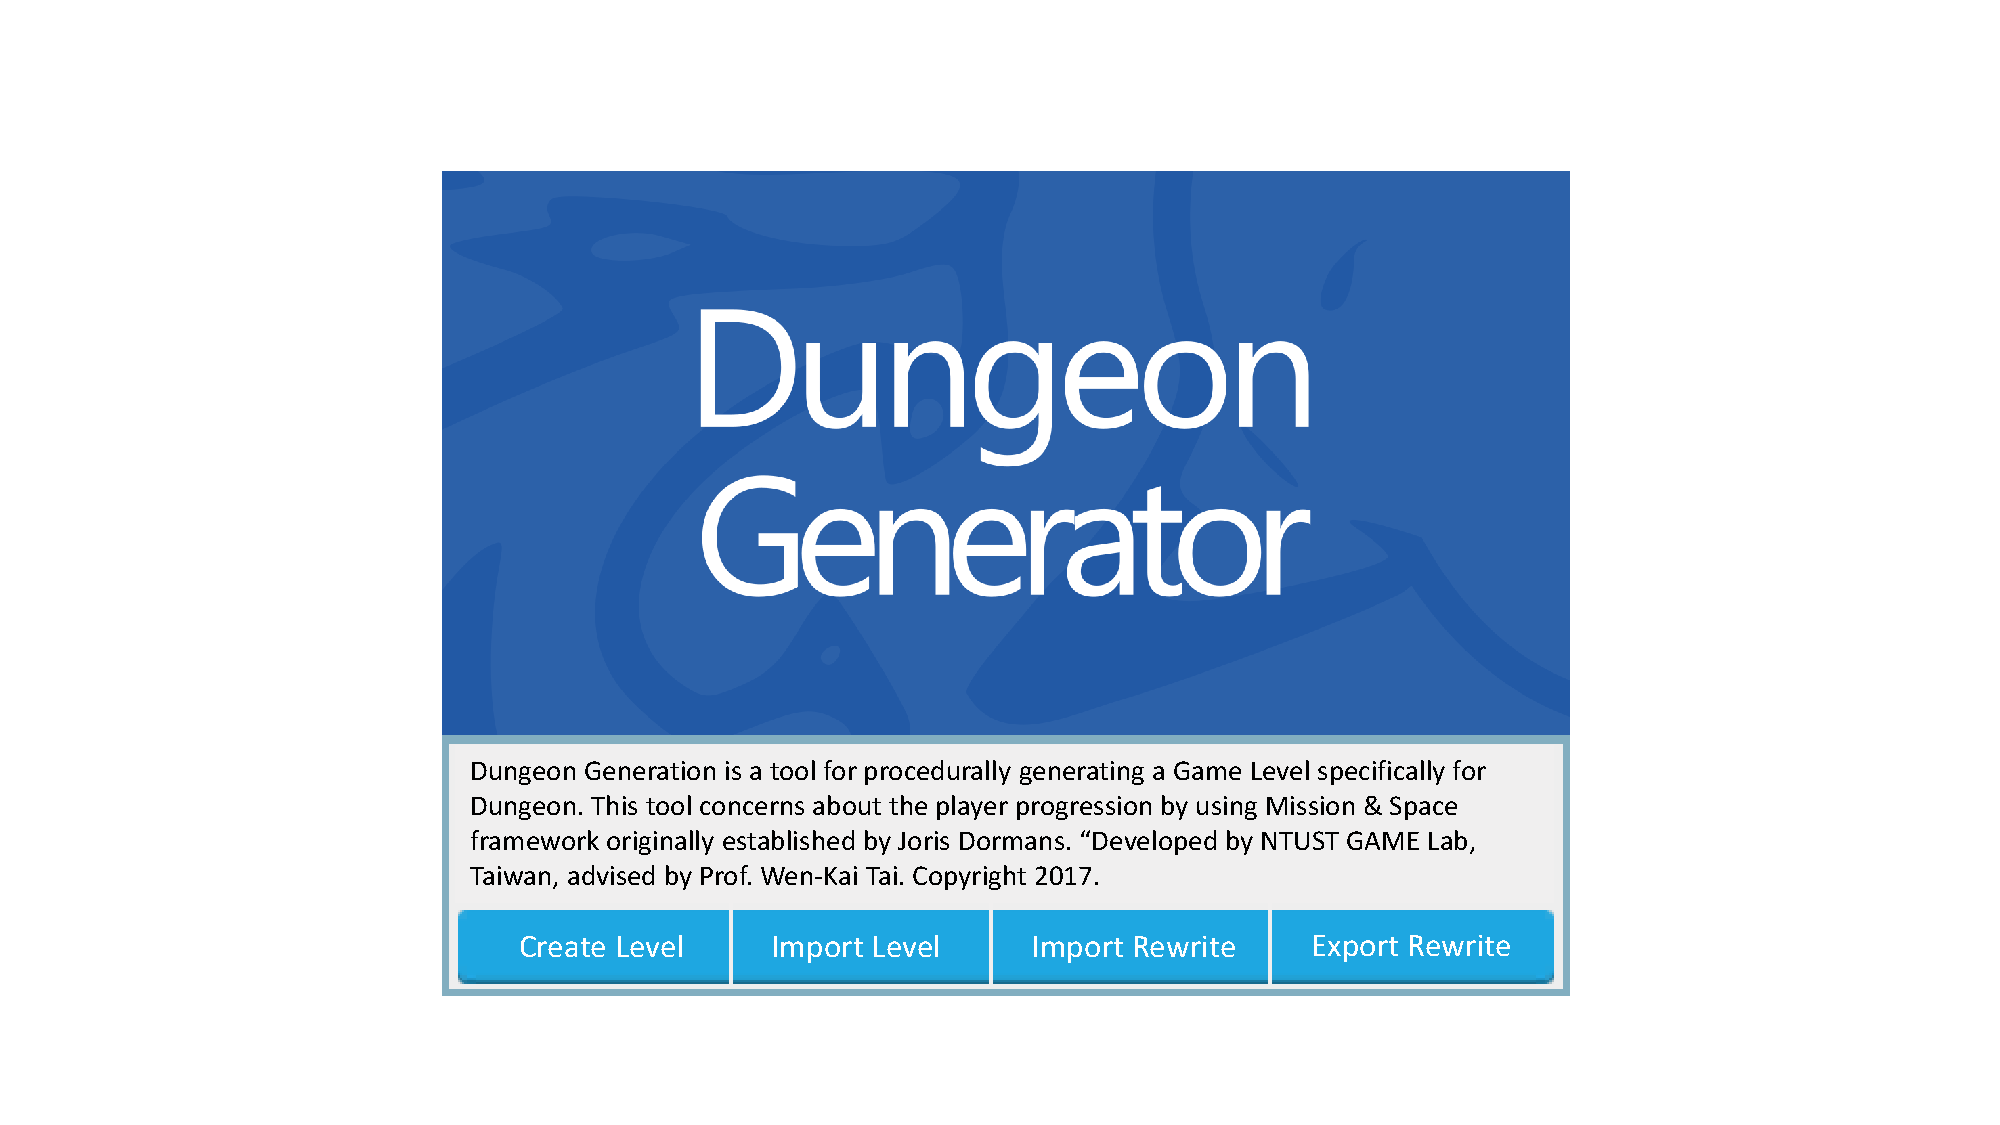
\includegraphics[width=1.0\textwidth]{figures/dungeon_generator.pdf}
    \caption{Dungeon Generator 工具} 
    \label{fig:dungeon-generator}
  \end{center}
\end{figure}

\subsection{建立任務符號表}
\label{ssec:method-missiongrammars-alphabet}

在本小節,會以\textit{The binding of Isaac} 遊戲關卡~\cite{isaacWikiRooms} 作為範例,解析其遊玩特徵並作為任務語法的節點。表~\ref{tbl:mission-grammars-alphabet-default} 為系統預設任務符號表。

\begin{table}[!htb]
  \centering
  \caption{系統預設的任務符號}
  \label{tbl:mission-grammars-alphabet-default}
  \bigskip
  \vspace{-5mm}
  \begin{tabular}{
    | >{\centering\arraybackslash} m{2.8cm}
    | >{\centering\arraybackslash} m{2.0cm}
    | >{\centering\arraybackslash} m{1.0cm}
    | >{\arraybackslash} m{6.7cm} | }
    \hline
    \multicolumn{1}{ |c| }{代號}
      & \multicolumn{1}{ c| }{名稱}
      & \multicolumn{1}{ c| }{符號}
      & \multicolumn{1}{ c| }{說明} \\\hline
    en (entrance)
      & 起點
      & \missionalphabetnode{t-entrance}{10mm}
      & 玩家於遊戲關卡開始時的起始位置。
      \\\hline
    go (goal)
      & 終點
      & \missionalphabetnode{t-goal}{10mm}
      & 玩家抵達此位置時遊戲將結束。
      \\\hline
    ? (any)
      & 任一節點
      & \missionalphabetnode{sys-any}{10mm}
      & 此節點能夠被判別為任何節點,定義任務規則時有著特殊用途。於~\ref{ssec:method-missiongrammars-rules} 小節中,對其使用方式將進行闡述。
      \\\hline
  \end{tabular}
\end{table}

\subsubsection{解析遊玩特徵}
\label{sssec:method-missiongrammars-alphabet-extractpatterns}

在任務語法中,任務節點可表示為一項事件、挑戰、動作或遊戲物件等。藉由觀察 \textit{The binding of Isaac} 的遊戲關卡後,能夠發現房間擁有固定類型,並且對於房間之間進行程序化的排列組合。然而固定的房間類型便是我們所尋找的節點種類,表~\ref{tbl:mission-grammars-alphabet} 列舉利用遊玩特徵所建立的任務符號表,藉此歸納出「起點 (entrance\missionalphabetnode{t-entrance}{5mm})、終點 (goal\missionalphabetnode{t-goal}{5mm})、魔王房 (boss\missionalphabetnode{t-boss}{5mm})、一般房 (normal\missionalphabetnode{t-normal}{5mm})」外,以及一定機率會出現的稀有特殊房間「秘密房 (secret\missionalphabetnode{t-secret}{5mm})、商店 (shop\missionalphabetnode{t-shop}{5mm})、寶藏房 (treasure\missionalphabetnode{t-treasure}{5mm})」,其中起點與終點為系統預設之終端節點。這些稀有房間帶來了一些制式的事件,在進入秘密房前必須使用炸彈將牆壁給破壞的事件 (bomb\missionalphabetnode{t-bomb}{5mm}),以及從秘密房取得的鑰匙能夠進行解鎖 (lock\missionalphabetnode{t-lock}{5mm}),開通進入商店或寶藏房的權限。而前述的遊玩特徵將轉化為終端節點 (terminal nodes) 的圓形符號形式,表示較為詳盡的任務內容;另外一種為方形符號的非終端節點 (non-terminal nodes),相較於終端節點更為高階、抽象化,在此我們定義出起始節點 (Start\missionalphabetnode{nt-start}{5mm})、一般房 (Normal\missionalphabetnode{nt-normal}{5mm}) 與特殊房 (Special\missionalphabetnode{nt-special}{5mm}) 等,其應用方式將在下一小節~\ref{ssec:method-missiongrammars-rules} 中介紹。

\setlength\LTcapwidth{\linewidth}
\begin{longtable}{
    | >{\centering\arraybackslash} m{2.8cm}
    | >{\centering\arraybackslash} m{2.0cm}
    | >{\centering\arraybackslash} m{1.0cm}
    | >{\arraybackslash} m{4.7cm}
    | >{\centering\arraybackslash} m{2.0cm} | }
  \caption{利用遊玩特徵建立任務符號表之範例}\label{tbl:mission-grammars-alphabet} \\
  \hline
  代號 & 名稱 & 符號 & \multicolumn{1}{ c| }{說明} & 類型 \\
  \hline
  \endfirsthead
  \multicolumn{5}{c}%
  {\tablename\ \thetable\ -- \textit{接續前頁面}} \\
  \hline
  代號 & 名稱 & 符號 & \multicolumn{1}{ c| }{說明} & 類型 \\
  \hline
  \endhead
  \multicolumn{5}{r}{\textit{接續下頁面}} \\
  \endfoot
  \endlastfoot
  S (Start)
    & 起始節點
    & \missionalphabetnode{nt-start}{10mm}
    & 任務圖進入改寫階段時,系統預設的根節點。
    & 起始節點 \\\hline
  boss (boss)
    & 魔王房
    & \missionalphabetnode{t-boss}{10mm}
    & 房間中存在著較強大的怪物。
    & \multirow{5.5}{*}{ 主線任務 } \\\cline{1-4}
  NM (Normal)
    & 一般房
    & \missionalphabetnode{nt-normal}{10mm}
    & 一般房間,藉由其它規則替換成其它房間或事件。
    &  \\\cline{1-4}
  nm (normal)
    & 一般房
    & \missionalphabetnode{t-normal}{10mm}
    & 遊戲過程中經過的通道,經常出現在遊戲關卡中。
    &  \\\hline
  bomb (bomb)
    & 使用炸彈
    & \missionalphabetnode{t-bomb}{10mm}
    & 必須使用炸彈將石牆給破壞,破壞石牆後便可通過。
    & \multirow{10}{*}{ 特殊事件 } \\\cline{1-4}
    % 10 is special to centering.
  srt (secret)
    & 秘密房
    & \missionalphabetnode{t-secret}{10mm}
    & 能夠取得稀有道具鑰匙的房間。
    &  \\\cline{1-4}
  SP (Special)
    & 特殊房
    & \missionalphabetnode{nt-special}{10mm}
    & 特殊房間,藉由其它規則替換成不同的稀有房間。
    &  \\\cline{1-4}
  lock (lock)
    & 鎖
    & \missionalphabetnode{t-lock}{10mm}
    & 必須使用鑰匙才能夠通過該空間。
    &  \\\cline{1-4}
  shop (shop)
    & 商店
    & \missionalphabetnode{t-shop}{10mm}
    & 能夠觸發特殊事件,玩家能夠在此購買道具。
    &  \\\cline{1-4}
  ts (treasure)
    & 寶藏房
    & \missionalphabetnode{t-treasure}{10mm}
    & 藏有稀有道具的房間,當中會有守衛寶箱的敵人。
    &  \\\hline
\end{longtable}

% \subsubsection{任務符號表使用說明}
% \label{sssec:method-missiongrammars-alphabet-manual}

% content here.

% \begin{figure}[!htb]
%   \begin{center}
%     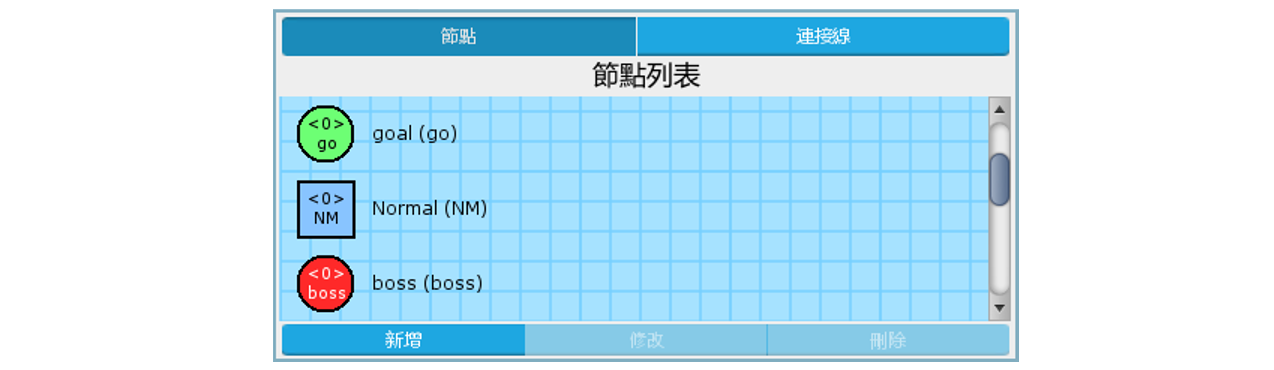
\includegraphics[width=1.0\textwidth]{figures/missiongrammars-alphabet-manual.png}
%     \caption{利用 Dungeon Generator 建立符號表} 
%     \label{fig:missiongrammars-alphabet-manual}
%   \end{center}
% \end{figure}

\subsection{建立任務規則}
\label{ssec:method-missiongrammars-rules}

圖~\ref{fig:missiongrammars-tutorial},任務規則分為規則左側及規則右側,二者皆為圖形語法 (Graph Grammars) 所構成,圖形與則由終端節點、非終端節點與連接線 (connection) 所構成的有向圖。規則左側為被取代方、規則右側為取代方,在任務圖中若有子圖符合任務規則的左側,將會依照流程進行替換改寫動作至規則右側,可參照第~\ref{ssec:method-missiongrammars-graph} 小節之說明。為了方便管理與分類不同性質的規則,在 \textit{Dungeon Generator} 中定義一任務語法包含了多個任務規則群組,各自群組底下有複數個任務改寫規則。

\begin{figure}[!htb]
  \begin{center}
    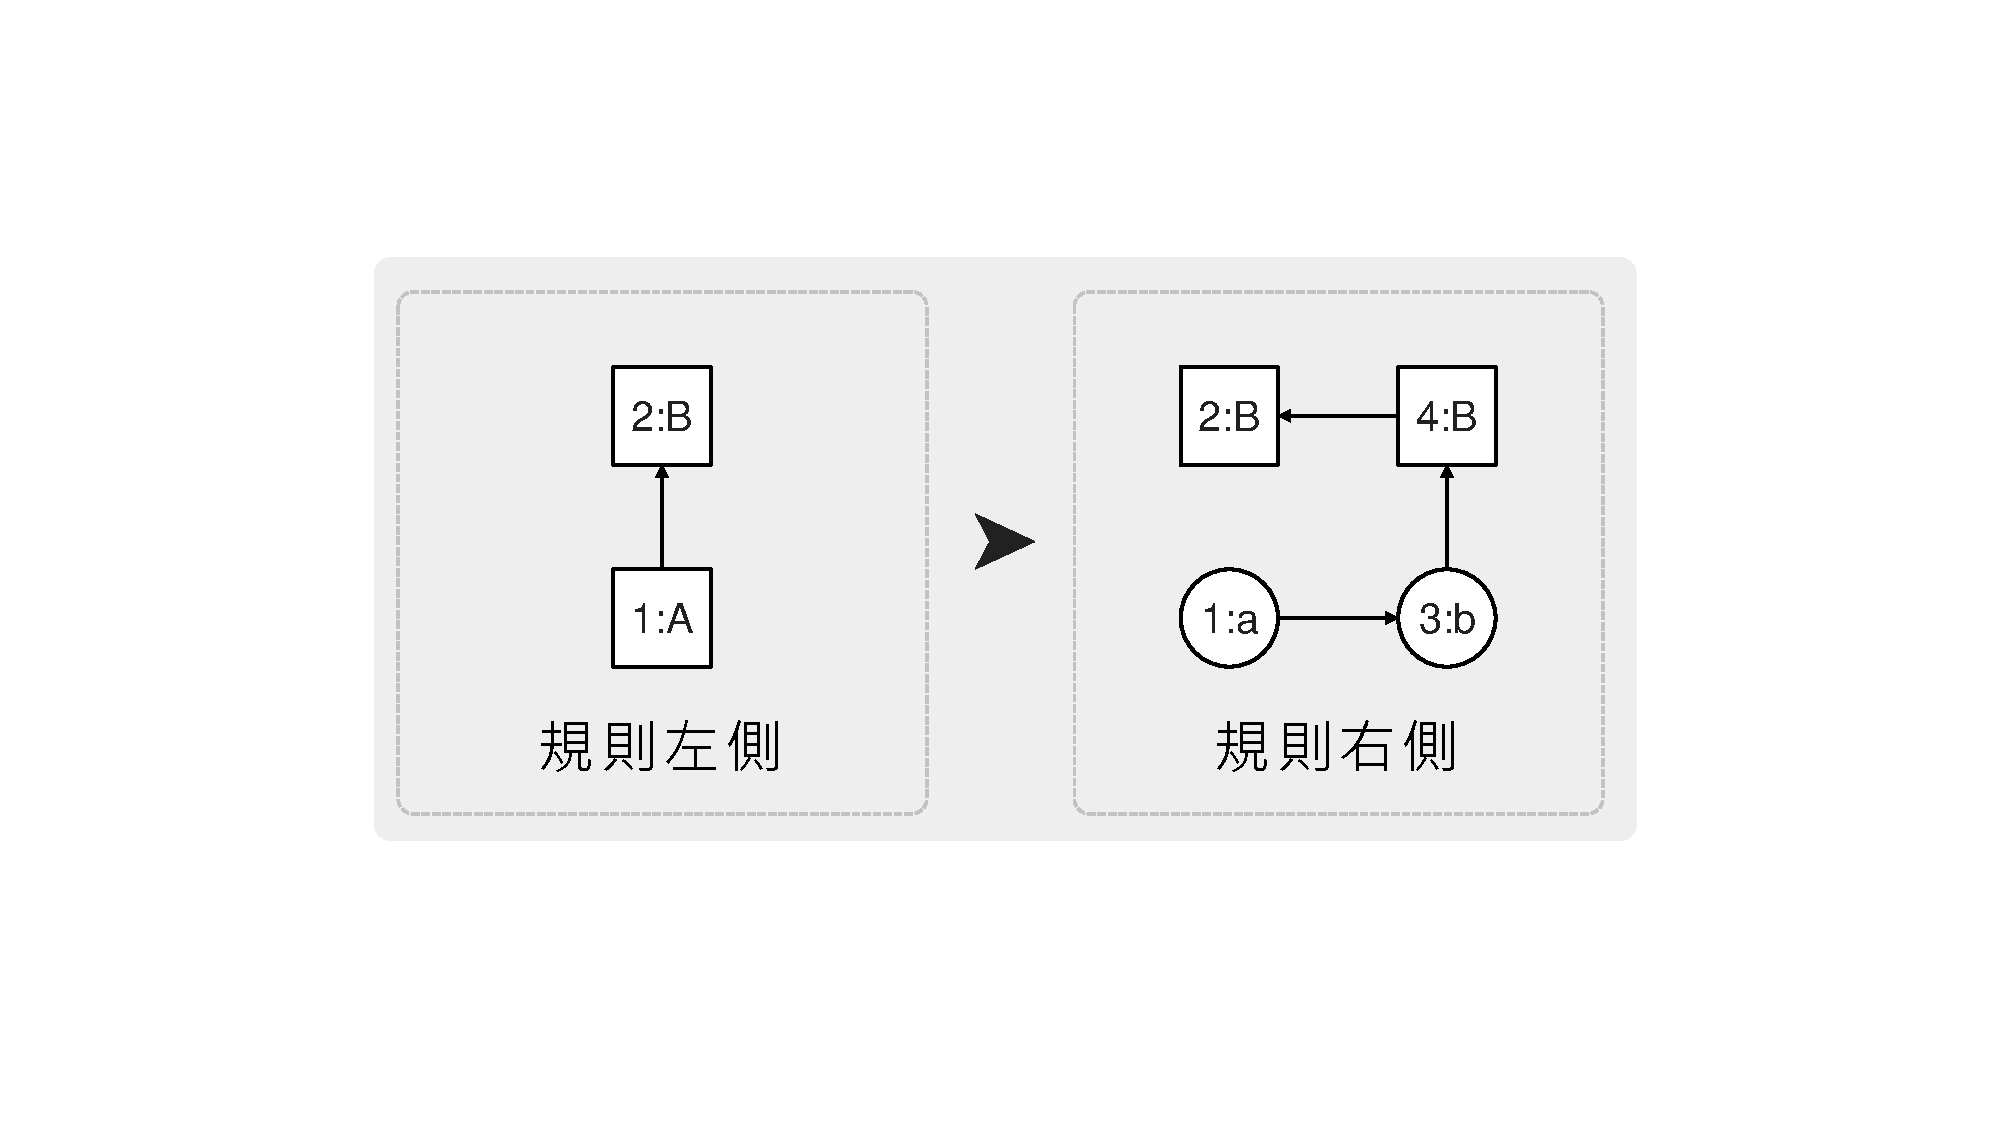
\includegraphics[width=1.0\textwidth]{figures/missiongrammars-tutorial.pdf}
    \caption{任務規則範例}
    \label{fig:missiongrammars-tutorial}
  \end{center}
\end{figure}

\subsubsection{線性任務規則}
\label{sssec:method-missiongrammars-rules-linearrules}

玩家在進行遊戲時,會有一條的主要任務流程、劇情安排。表~\ref{tbl:missiongrammars-rules-linear-example} 設計了三道任務規則,分別為主線任務、配置魔王房與探索通道。主線任務規則中,系統會從預設起始節點 (starting node) 開始進行改寫,並轉換為由終端節點起點 (entrance\missionalphabetnode{t-entrance}{5mm}) 與終點 (goal\missionalphabetnode{t-goal}{5mm}) 所構成的線性任務,其中兩節點之間由數個非終端節點的一般房 (Normal\missionalphabetnode{nt-normal}{5mm}) 相連,而非終端節點的一般房會倚賴其它規則進行後續替換。配置魔王房規則中,規則左側中定義了必須為非終端節點的一般房 (Normal\missionalphabetnode{nt-normal}{5mm}) 與終點 (goal\missionalphabetnode{t-goal}{5mm}) 相連,並改寫該一般房為魔王房 (boss\missionalphabetnode{t-boss}{5mm})。探索通道規則中,會將任務圖中的剩餘非終端節點的一般房 (Normal\missionalphabetnode{nt-normal}{5mm}) 替換為終端節點的一般房 (normal\missionalphabetnode{t-normal}{5mm})。

\begin{table}[!htb]
  \centering
  \caption{線性任務規則範例,建立主線任務}
  \label{tbl:missiongrammars-rules-linear-example}
  \bigskip
  \vspace{-5mm}
  \begin{tabular}{
    | >{\centering\arraybackslash} m{2.5cm}
    | >{\centering\arraybackslash} m{2.5cm}
      >{} m{8.5cm} | }
    \hline
    \multicolumn{1}{ |c| }{代號}
      & \multicolumn{2}{ c| }{名稱與任務規則} \\\hline
    Main Path
      & 主線任務
      & \begin{minipage}{.3\textwidth}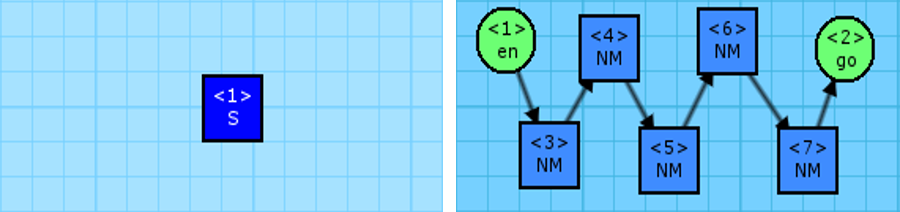
\includegraphics[width=85mm]{figures/mission-grammars-rules/main-path.png}\end{minipage}
      \\\hline
    Boss Room
      & 配置魔王房
      & \begin{minipage}{.3\textwidth}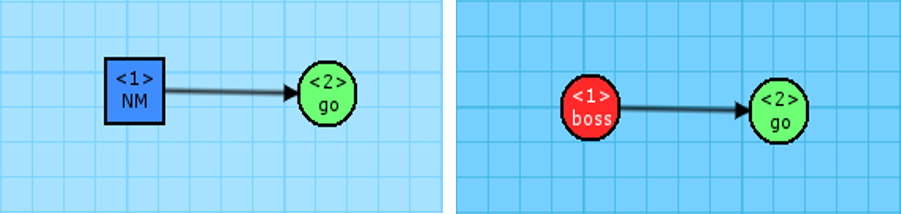
\includegraphics[width=85mm]{figures/mission-grammars-rules/boss-room.png}\end{minipage}
      \\\hline
    Exporation
      & 探索通道
      & \begin{minipage}{.3\textwidth}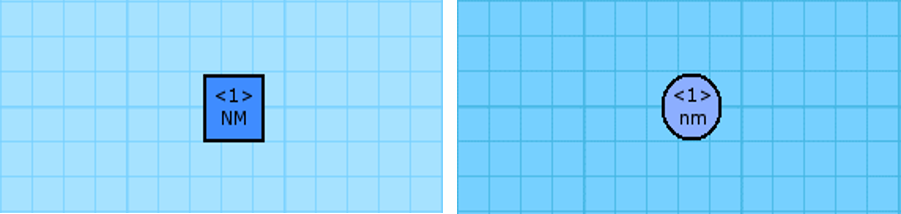
\includegraphics[width=85mm]{figures/mission-grammars-rules/exporation.png}\end{minipage}
      \\\hline
  \end{tabular}
\end{table}

結合後續第~\ref{sec:method-spacepieces} 章節 - 空間建構,並以主線任務相關規則生成任務圖後,便可將關卡輸出近似於圖~\ref{fig:missiongrammars-rules-linear-preview} 的空間。

\begin{figure}[!htb]
  \begin{center}
    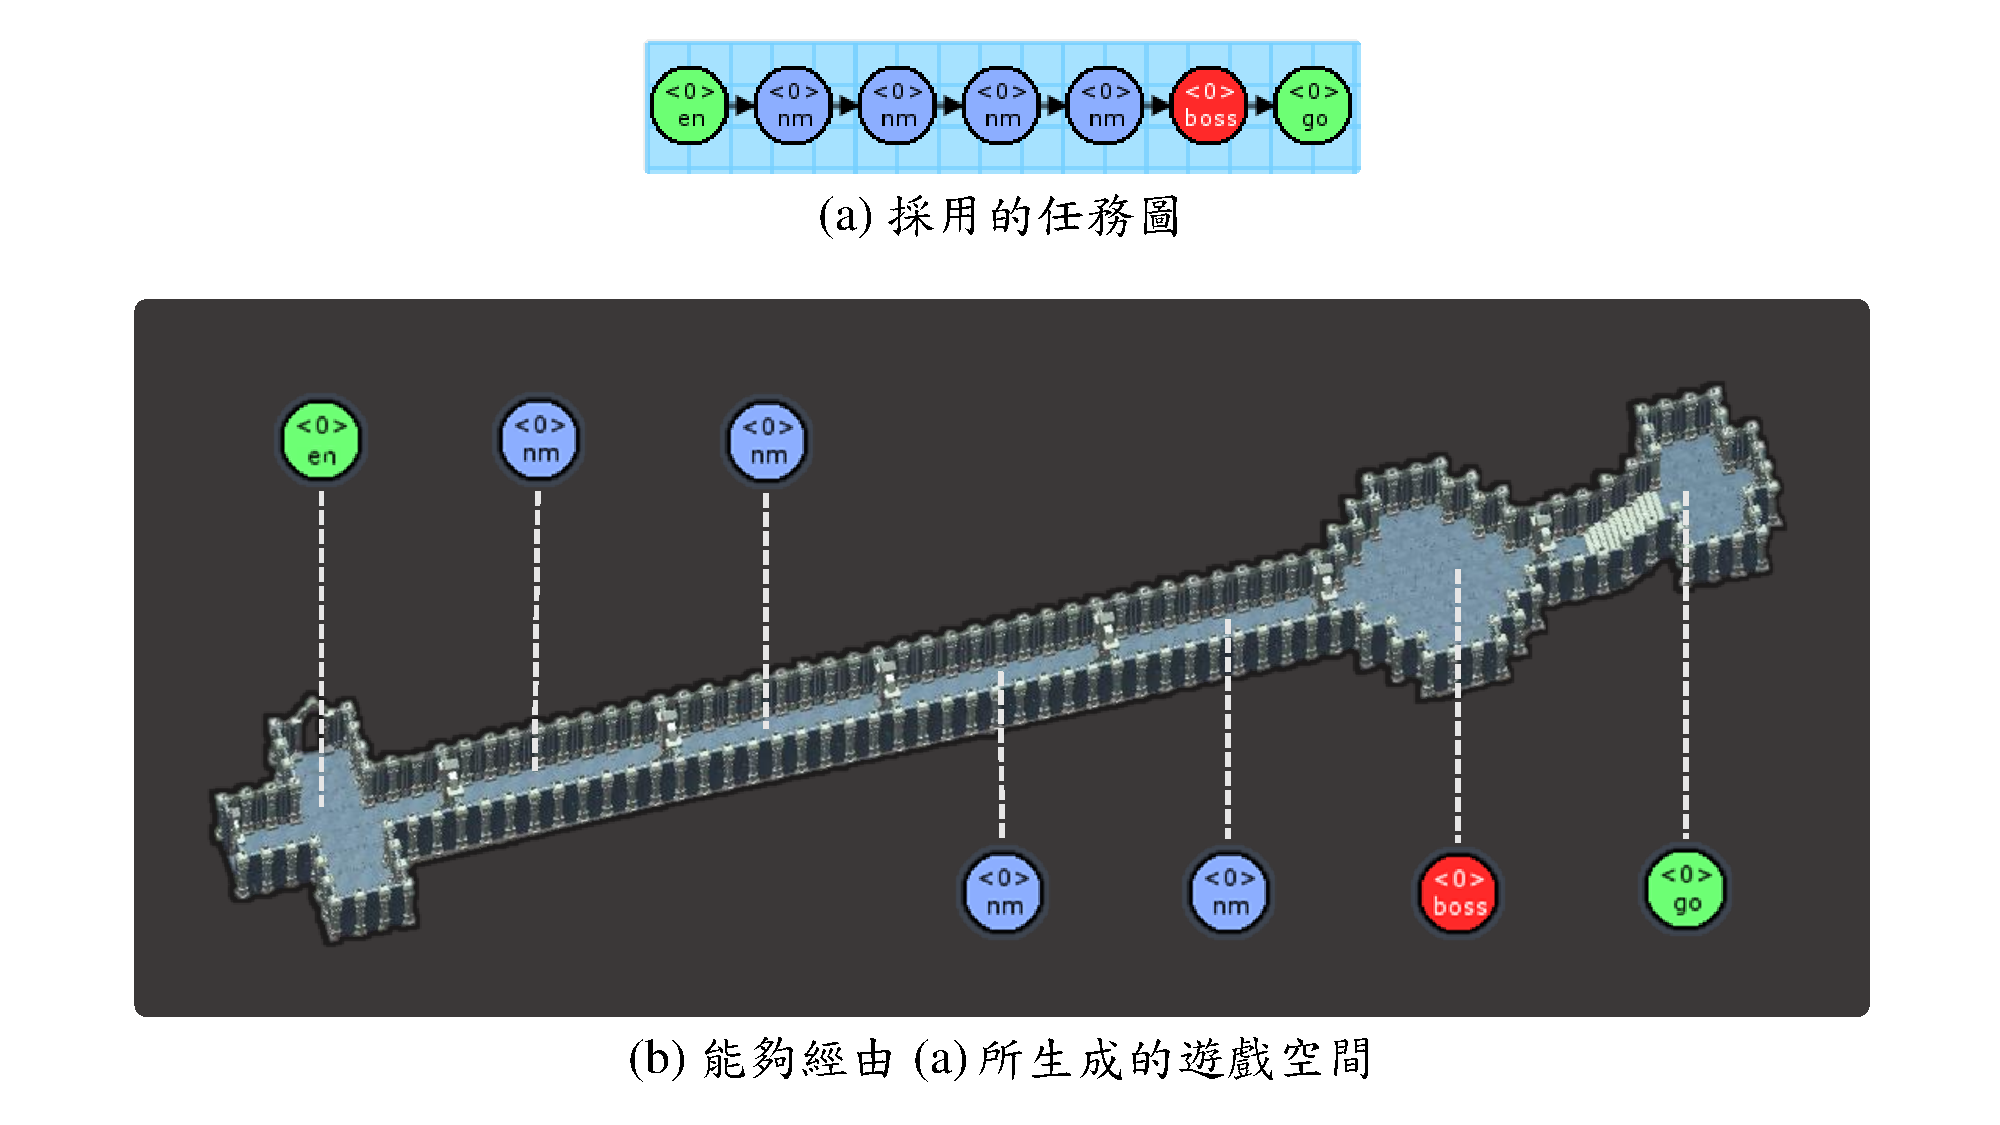
\includegraphics[width=1.0\textwidth]{figures/missiongrammars-rules-linear-preview.pdf}
    \caption{建立主線任務的預期任務圖與空間預覽}
    \label{fig:missiongrammars-rules-linear-preview}
  \end{center}
\end{figure}

\subsubsection{非線性任務規則}
\label{sssec:method-missiongrammars-rules-nonlinearrules}

為求遊戲內容的多樣性,非終端節點的一般房 (Normal\missionalphabetnode{nt-normal}{5mm}) 將有機會轉換為其它種類的遊玩特徵,表~\ref{tbl:missiongrammars-rules-nonlinear-example1} 定義了特殊房間的配置工作。配置特殊房規則中,非終端節點的一般房 (Normal\missionalphabetnode{nt-normal}{5mm}) 與任一節點相連的圖形語法(任一節點是系統保留的節點,再圖形語法中能夠表示任何的節點),會被轉換為規則右側的非線性任務圖形語法,非線性的定義是當一個節點與複數個節點連接,構成分支結構,當中的秘密房 (secret\missionalphabetnode{t-secret}{5mm}) 能夠獲取鑰匙,並有需要由炸彈才能夠突破的牆壁 (bomb\missionalphabetnode{t-bomb}{5mm}) 與其它區域阻隔,此外延伸出特殊房 (Special\missionalphabetnode{nt-special}{5mm}) 需另外定義規則使之轉換為終端節點。由於這項規則屬於較為稀少的任務類型,在套用數量上將有所限制。在商店規則與寶藏房規則中,規則左側中定義了非終端節點的特殊房 (Special\missionalphabetnode{nt-special}{5mm}) 能夠被改寫為鎖 (lock\missionalphabetnode{t-lock}{5mm}) 與商店 (shop\missionalphabetnode{t-shop}{5mm}) 或寶藏房 (treasure\missionalphabetnode{t-treasure}{5mm}) 相連的遊玩特徵。

\begin{table}[!htb]
  \centering
  \caption{非線性任務規則範例,設置特殊房}
  \label{tbl:missiongrammars-rules-nonlinear-example1}
  \bigskip
  \vspace{-5mm}
  \begin{tabular}{
    | >{\centering\arraybackslash} m{2.5cm}
    | >{\centering\arraybackslash} m{2.5cm}
      >{} m{8.5cm} | }
    \hline
    \multicolumn{1}{ |c| }{代號}
      & \multicolumn{2}{ c| }{名稱與任務規則} \\\hline
    Set Secret
      & 配置特殊房
      & \begin{minipage}{.3\textwidth}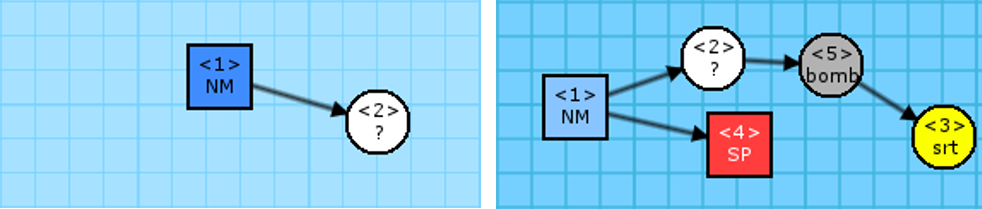
\includegraphics[width=85mm]{figures/mission-grammars-rules/set-secret.png}\end{minipage}
      \\\hline
    Shop
      & 商店
      & \begin{minipage}{.3\textwidth}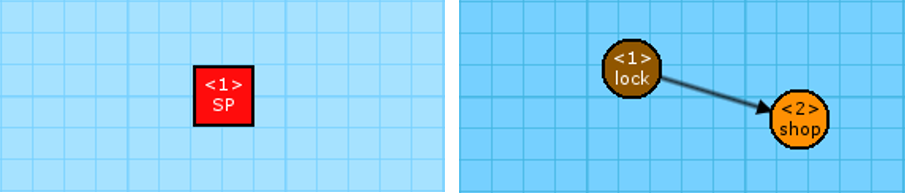
\includegraphics[width=85mm]{figures/mission-grammars-rules/shop.png}\end{minipage}
      \\\hline
    Treasure
      & 寶藏房
      & \begin{minipage}{.3\textwidth}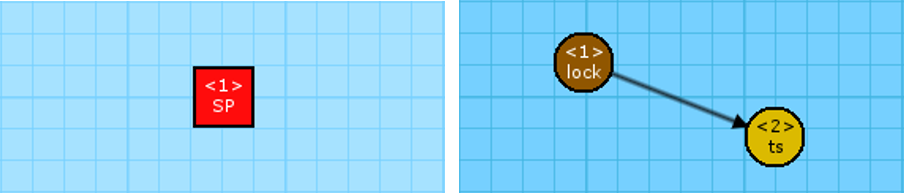
\includegraphics[width=85mm]{figures/mission-grammars-rules/treasure.png}\end{minipage}
      \\\hline
  \end{tabular}
\end{table}

表~\ref{tbl:missiongrammars-rules-nonlinear-example2},建立支線任務規則能讓指定的節點額外分支出支線任務,替換後的非終端節點一般房 (Normal\missionalphabetnode{nt-normal}{5mm}) 便能再經過其它的規則,取代成不同的遊玩特徵。

\begin{table}[!htb]
  \centering
  \caption{非線性任務規則範例,建立支線任務}
  \label{tbl:missiongrammars-rules-nonlinear-example2}
  \bigskip
  \vspace{-5mm}
  \begin{tabular}{
    | >{\centering\arraybackslash} m{2.5cm}
    | >{\centering\arraybackslash} m{2.5cm}
      >{} m{8.5cm} | }
    \hline
    \multicolumn{1}{ |c| }{代號}
      & \multicolumn{2}{ c| }{名稱與任務規則} \\\hline
    More Branch
      & 建立支線
      & \begin{minipage}{.3\textwidth}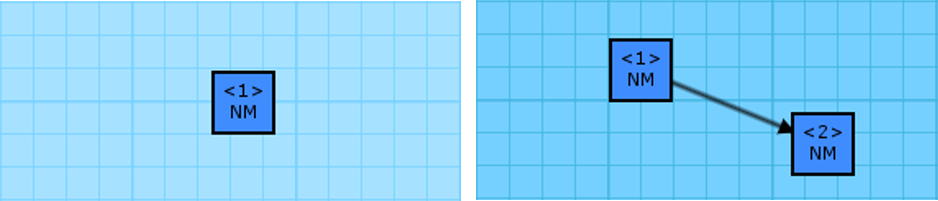
\includegraphics[width=85mm]{figures/mission-grammars-rules/more-branch.png}\end{minipage}
      \\\hline
  \end{tabular}
\end{table}

表~\ref{tbl:missiongrammars-rules-nonlinear-example3},為使玩家進行遊戲能夠提前遇見鎖 (lock\missionalphabetnode{t-lock}{5mm}),當下卻找不到鑰匙的遊玩特徵,進而思考、尋找開鎖的方式,便利用鎖向前規則將鎖的分支一同往前挪動。房間攤平規則,為避免單一房間與過多的房間連通,將部分房間進行移前推挪。

\begin{table}[!htb]
  \centering
  \caption{非線性任務規則範例,鎖的提前出現與房間攤平}
  \label{tbl:missiongrammars-rules-nonlinear-example3}
  \bigskip
  \vspace{-5mm}
  \begin{tabular}{
    | >{\centering\arraybackslash} m{2.5cm}
    | >{\centering\arraybackslash} m{2.5cm}
      >{} m{8.5cm} | }
    \hline
    \multicolumn{1}{ |c| }{代號}
      & \multicolumn{2}{ c| }{名稱與任務規則} \\\hline
    Forward Lock
      & 鎖向前
      & \begin{minipage}{.3\textwidth}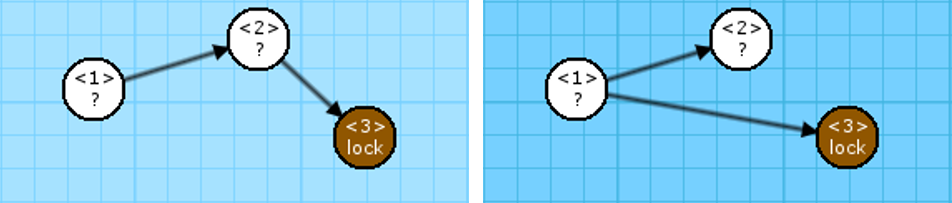
\includegraphics[width=85mm]{figures/mission-grammars-rules/forward-lock.png}\end{minipage}
      \\\hline
    Flat Rooms
      & 房間攤平
      & \begin{minipage}{.3\textwidth}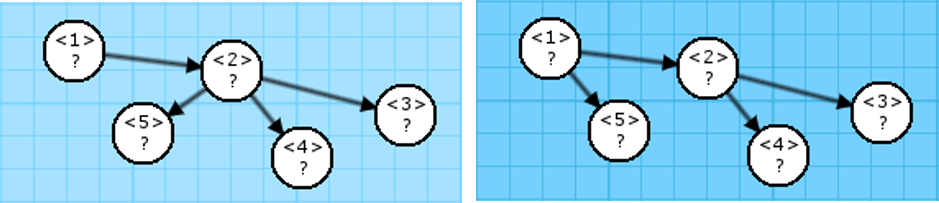
\includegraphics[width=85mm]{figures/mission-grammars-rules/flat-rooms.png}\end{minipage}
      \\\hline
  \end{tabular}
\end{table}

% \subsubsection{重複循環型任務規則}
% \label{sssec:method-missiongrammars-rules-cyclic}

% 遊戲設計師能夠依照需求定義出無窮的疊代規則,舉例來說,

\subsubsection{排除非法規則}
\label{sssec:method-missiongrammars-rules-illegals}

設計規則時,\textit{Dungeon Generator} 將排除不合法的九項設計原則,非法的設計特徵會導致改寫系統出現錯誤,見圖~\ref{fig:missiongrammars-illegal-rules}。例如:改寫系統陷入無限循環或任務圖破碎化。在表~\ref{tbl:illegal-mission-rules} 所列舉之條件於某些情況中,可能彼此會同時符合多項非法條件,系統將依照判斷順序擇一輸出。

\begin{figure}[!htb]
  \begin{center}
    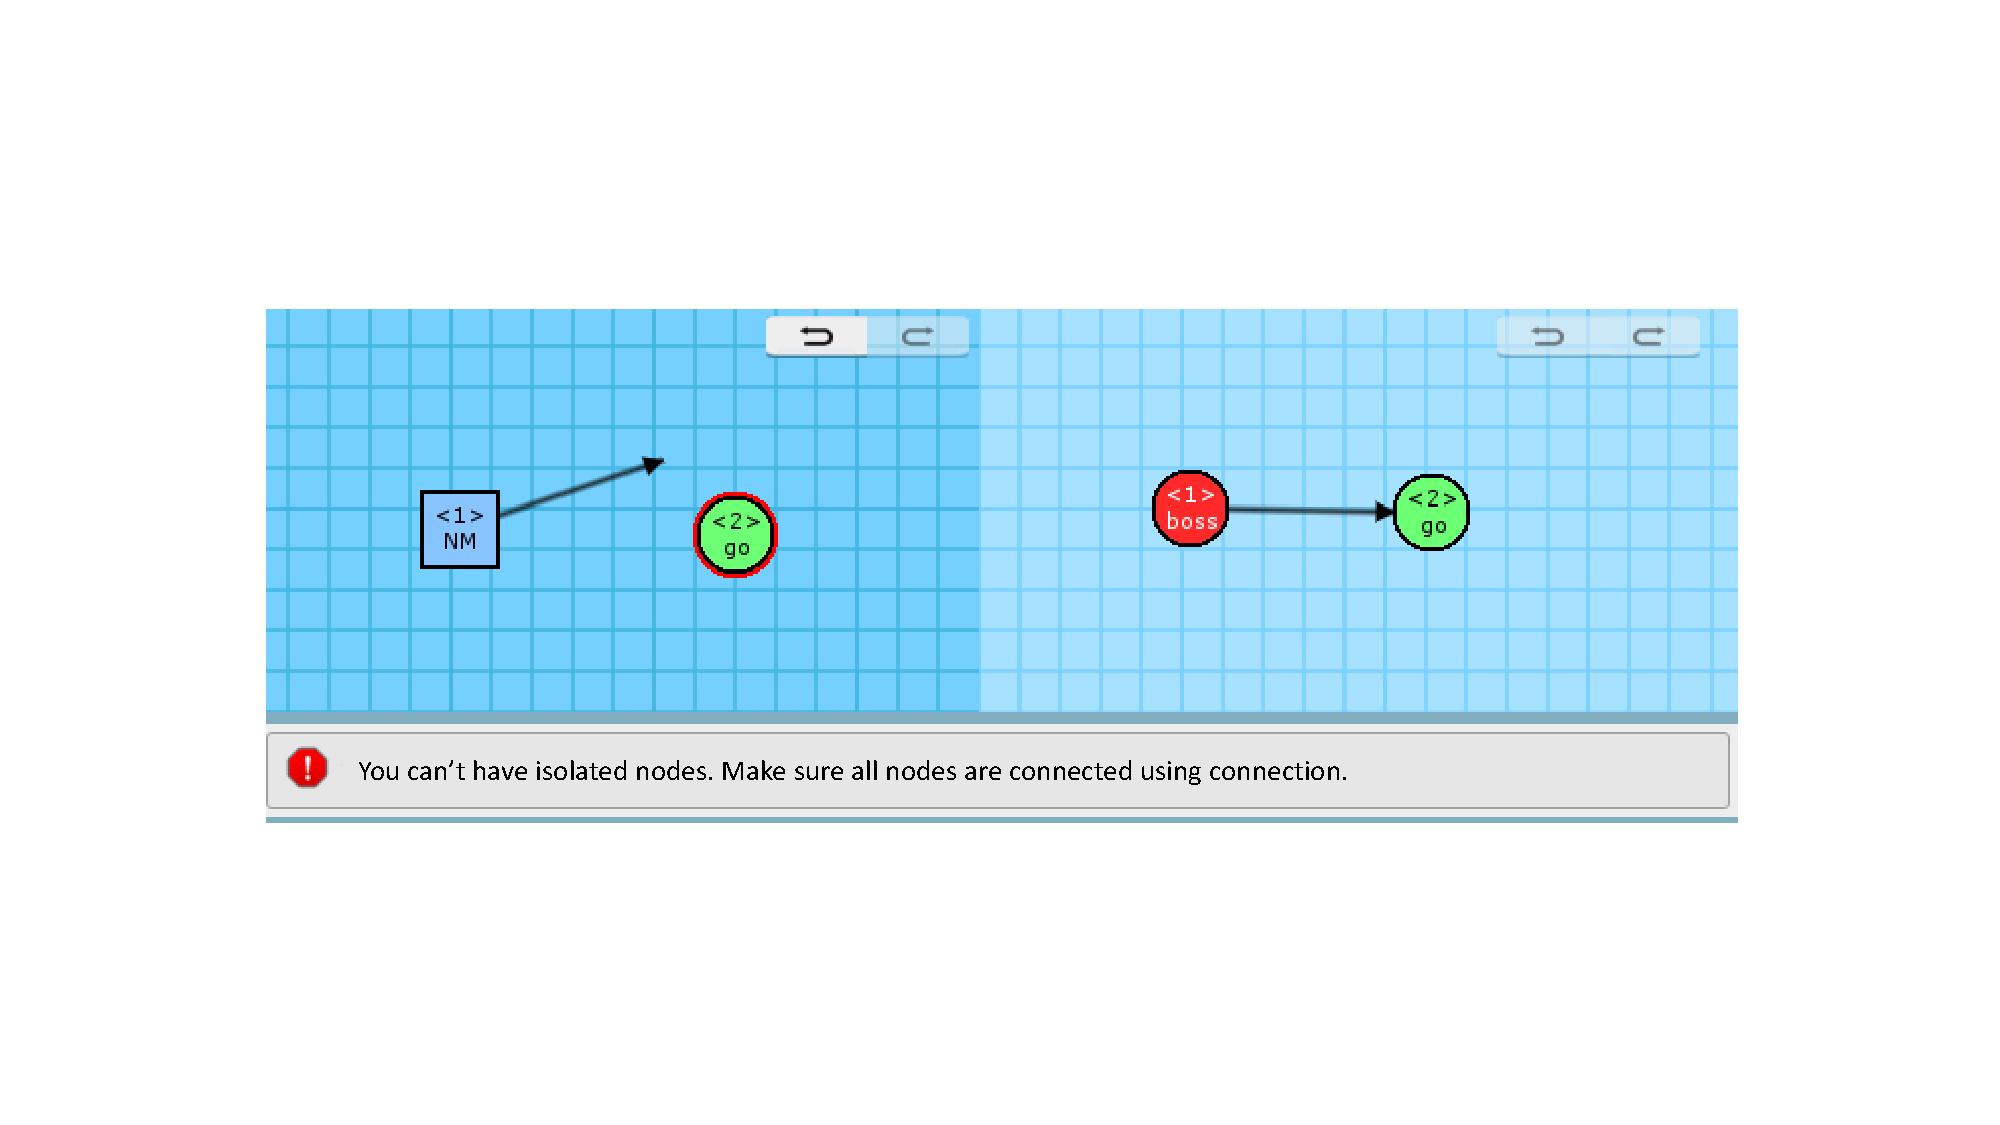
\includegraphics[width=1.0\textwidth]{figures/missiongrammars-illegal-rules.pdf}
    \caption{於 Dungeon Generator 工具中,若規則為非法狀態將不予生效}
    \label{fig:missiongrammars-illegal-rules}
  \end{center}
\end{figure}

\setlength\LTcapwidth{\linewidth}
\begin{longtable}{
    | >{\centering\arraybackslash} p{4cm}
    | >{} p{10cm} | }
  \caption{非法的任務規則定義}\label{tbl:illegal-mission-rules} \\
  \hline
  非法規則之標籤 & \multicolumn{1}{ c| }{標籤的狀況描述} \\
  \hline
  \endfirsthead
  \multicolumn{2}{c}%
  {\tablename\ \thetable\ -- \textit{接續前頁面}} \\
  \hline
  非法規則之標籤 & \multicolumn{1}{ c| }{標籤的狀況描述} \\
  \hline
  \endhead
  \multicolumn{2}{r}{\textit{接續下頁面}} \\
  \endfoot
  \endlastfoot
  LeftMoreThanRight  & 當左側的節點超過右側的節點數量時,進行改寫系統會使左側無法對應到右側的節點產生遺失的情形。若這些節點原先已有與其它非規則內節點連接,將會導致該連接資訊遺失,有機會造成任務圖破碎。 \\\hline
  EmptyLeft          & 左側為空將無法進行子圖搜索,因此左側節點必須至少一個節點。 \\\hline
  IsolatedNode       & 孤立的節點將會導致任務圖破碎。 \\\hline
  IsolatedConnection & 孤立的連接線無法正確表示其連接資訊,將無法正常進行改寫系統。 \\\hline
  ExactlyDuplicated  & 若左右規則同構將導致改寫系統陷入無限循環。 \\\hline
  MultipleRelations  & 兩兩節點間不可有超過一個的連接關係,不論是同向連接線或反向連接線皆會導致改寫系統無法正常運作。 \\\hline
  CyclicLink         & 任務圖的定義中,任務應嚴格遵守任務間之順序性,若有循環結構將會使玩家迂迴停滯。 \\\hline
  OrphanNode         & 若有圖形語法含有兩個以上的根節點,便無法正確定位出任務起點。 \\\hline
  OverflowedAnyNode  & 當規則右側使用 Any 節點時,其對應到左側索引值的節點亦必須為 Any 節點。反之,規則左側使用 Any 節點將不在此限。 \\\hline
\end{longtable}

\subsubsection{關聯權重與數量限制}
\label{sssec:method-missiongrammars-rules-relativeweight-quantitylimit}

「關聯權重 (relative weight) 」與「數量限制」提供 \textit{Dungeon Generator} 在設計任務規則時更多地彈性,關卡設計師能夠針調整特定的任務規則被套用的機率與套用的次數。任務規則被賦予使用數量上的條件限制,分為使用上限次數與下限次數,上限次數表示完整的改寫系統運行過程,最多能夠套用該規則的次數上限,多為了因應部分遊玩特徵的獨特性或稀有性;反之,下限次數表示套用該規則的次數下限,能用於改寫系統的疊代結果已趨於穩定、無剩餘任何非終端節點的情形下,作為持續進行改寫系統的強制約束條件。

表~\ref{tbl:mission-rules-relative-weight} 是基於任務規則表(表~\ref{tbl:missiongrammars-rules-linear-example} - ~\ref{tbl:missiongrammars-rules-nonlinear-example3})所建立的關聯權重表,關聯權重是一自然常數,當改寫系統進行時,會依照關聯權重與選定方法挑選出一任務規則。於下一小節中,關於關聯權重有詳細的解釋。

\setlength\LTcapwidth{\linewidth}
\begin{longtable}{
    | >{\centering\arraybackslash} p{4cm}
    | >{\centering\arraybackslash} p{4cm}
    | >{\centering\arraybackslash} p{2.75cm}
    | >{\centering\arraybackslash} p{2.75cm} | }
  \caption{關聯權重表,任務規則的關聯權重與數量設定之範例}\label{tbl:mission-rules-relative-weight} \\
  \hline
  任務規則代號 & 任務規則名稱 & 關聯權重 & 數量限制 \\
  \hline
  \endfirsthead
  \multicolumn{4}{c}%
  {\tablename\ \thetable\ -- \textit{接續前頁面}} \\
  \hline
  任務規則代號 & 任務規則名稱 & 關聯權重 & 數量限制 \\
  \hline
  \endhead
  \multicolumn{4}{r}{\textit{接續下頁面}} \\
  \endfoot
  \endlastfoot
  Main Path    & 主線任務   & $10$  & $[0,\infty]$ \\\hline
  Boss Room    & 配置魔王房 & $150$ & $[0,1]$      \\\hline
  Exporation   & 探索通道   & $10$  & $[0,\infty]$ \\\hline
  Set Secret   & 配置特殊房 & $30$  & $[0,1]$      \\\hline
  Shop         & 商店       & $10$  & $[0,1]$      \\\hline
  Treasure     & 寶藏房     & $10$  & $[0,1]$      \\\hline
  More Branch  & 建立支線   & $20$  & $[0,2]$      \\\hline
  Forward Lock & 鎖向前     & $10$  & $[0,2]$      \\\hline
  Flat Rooms   & 房間攤平   & $10$  & $[0,\infty]$ \\\hline
\end{longtable}

\subsection{產生任務圖}
\label{ssec:method-missiongrammars-graph}

上一小節中定義了任務規則,本小節將利用任務規則進行生成任務圖的步驟。我們參考 Joris Dormans~\cite{dormans2010adventures} 提出的方法並改良之,歸納出演算法~\ref{alg:algorithm-missiongrammars-rewritesystem} - 改寫系統(任務語法)與演算法~\ref{alg:algorithm-matchedrule} - 搜尋匹配規則。圖~\ref{fig:rewrite-system-i-flow},任務語法的改寫系統運行時,以深度優先搜尋法 (Depth-first search) 遍歷整個任務圖。

圖~\ref{fig:rewrite-system-i-flow} a,源節點會從任務規則集合中過濾出相符的規則,若有多項規則同時符合替換的條件時,系統會基於它們的關聯權重,從複數個規則中依照採輪盤法 (roulette wheel selection)~\cite{lipowski2012roulette} 選擇出一項任務規則稱之為匹配規則 (matched rule),並從源節點進行與匹配規則的改寫替換。符合的條件為定義遍歷中的源節點作為新圖,而新圖存在一個子圖與匹配規則的左側之圖形語法同構,同構的參考基準為節點的符號種類,見圖~\ref{fig:rewrite-system-isomorphic}。在確認子圖同構的同時,有關連的節點會標記與匹配規則一致的索引值。圖~\ref{fig:rewrite-system-i-flow} b,將任務圖含有索引值的節點,其相連的連接線移除。圖~\ref{fig:rewrite-system-i-flow} c,任務圖含有有索引值的節點(\textbf{1:A} 與 \textbf{2:B})取代成匹配規則右側的等價節點(\textbf{1:a} 與 \textbf{2:B})。圖~\ref{fig:rewrite-system-i-flow} d,索引值編號為 \textbf{3} 與 \textbf{4} 的節點僅出現於匹配規則右側,於是將匹配規則右側中沒有與左側等價的節點(\textbf{3:b} 與 \textbf{4:B})添加至任務圖中。圖~\ref{fig:rewrite-system-i-flow} e,依照匹配規則右側的連接線,以相同方式放入任務圖中。圖~\ref{fig:rewrite-system-i-flow} f,將任務圖中的索引值屬性移除。

\begin{figure}[!htb]
  \begin{center}
    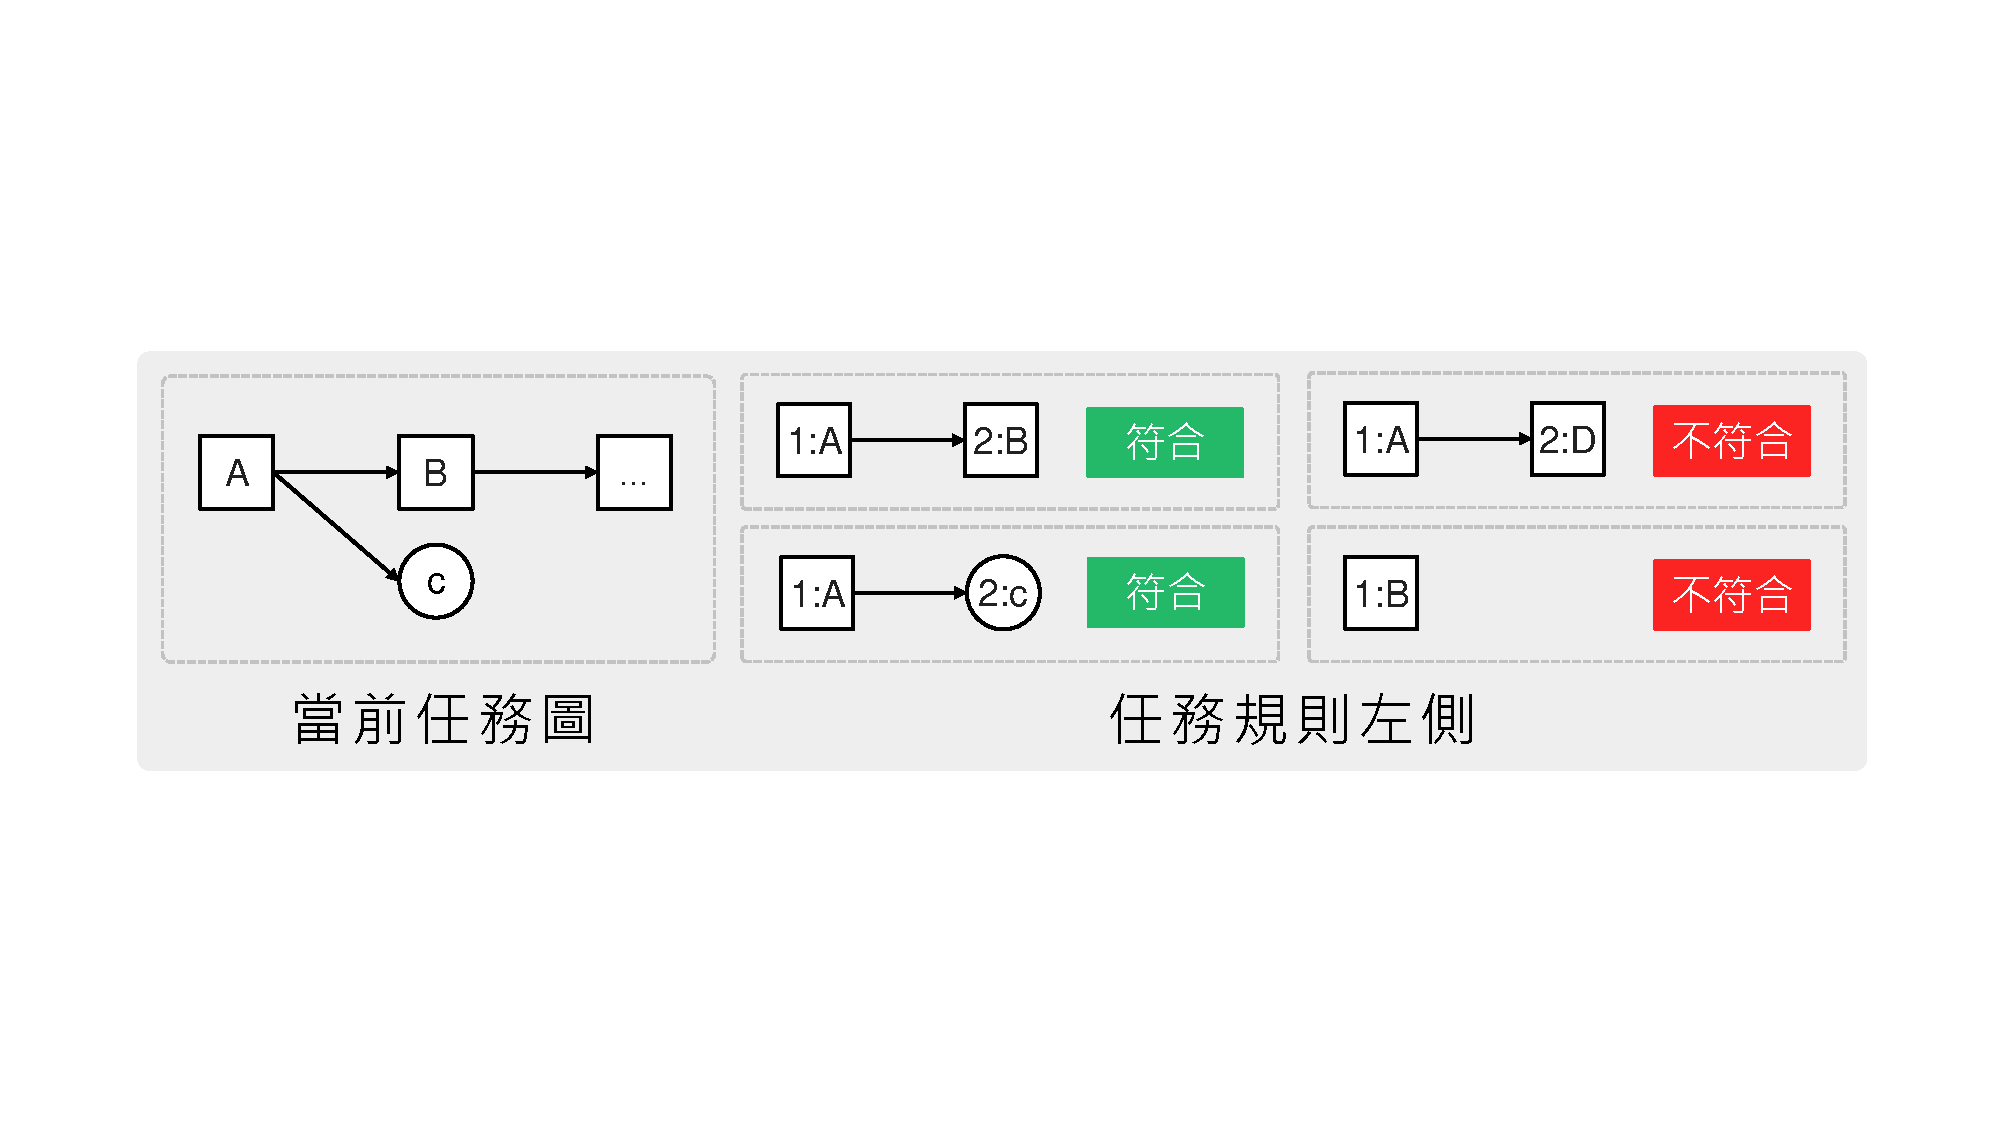
\includegraphics[width=1.0\textwidth]{figures/rewrite-system-isomorphic.pdf}
    \caption{匹配規則的子圖同構判定方式示意,當前根節點為 \textbf{A}}
    \label{fig:rewrite-system-isomorphic}
  \end{center}
\end{figure}

\begin{figure}[!htb]
  \begin{center}
    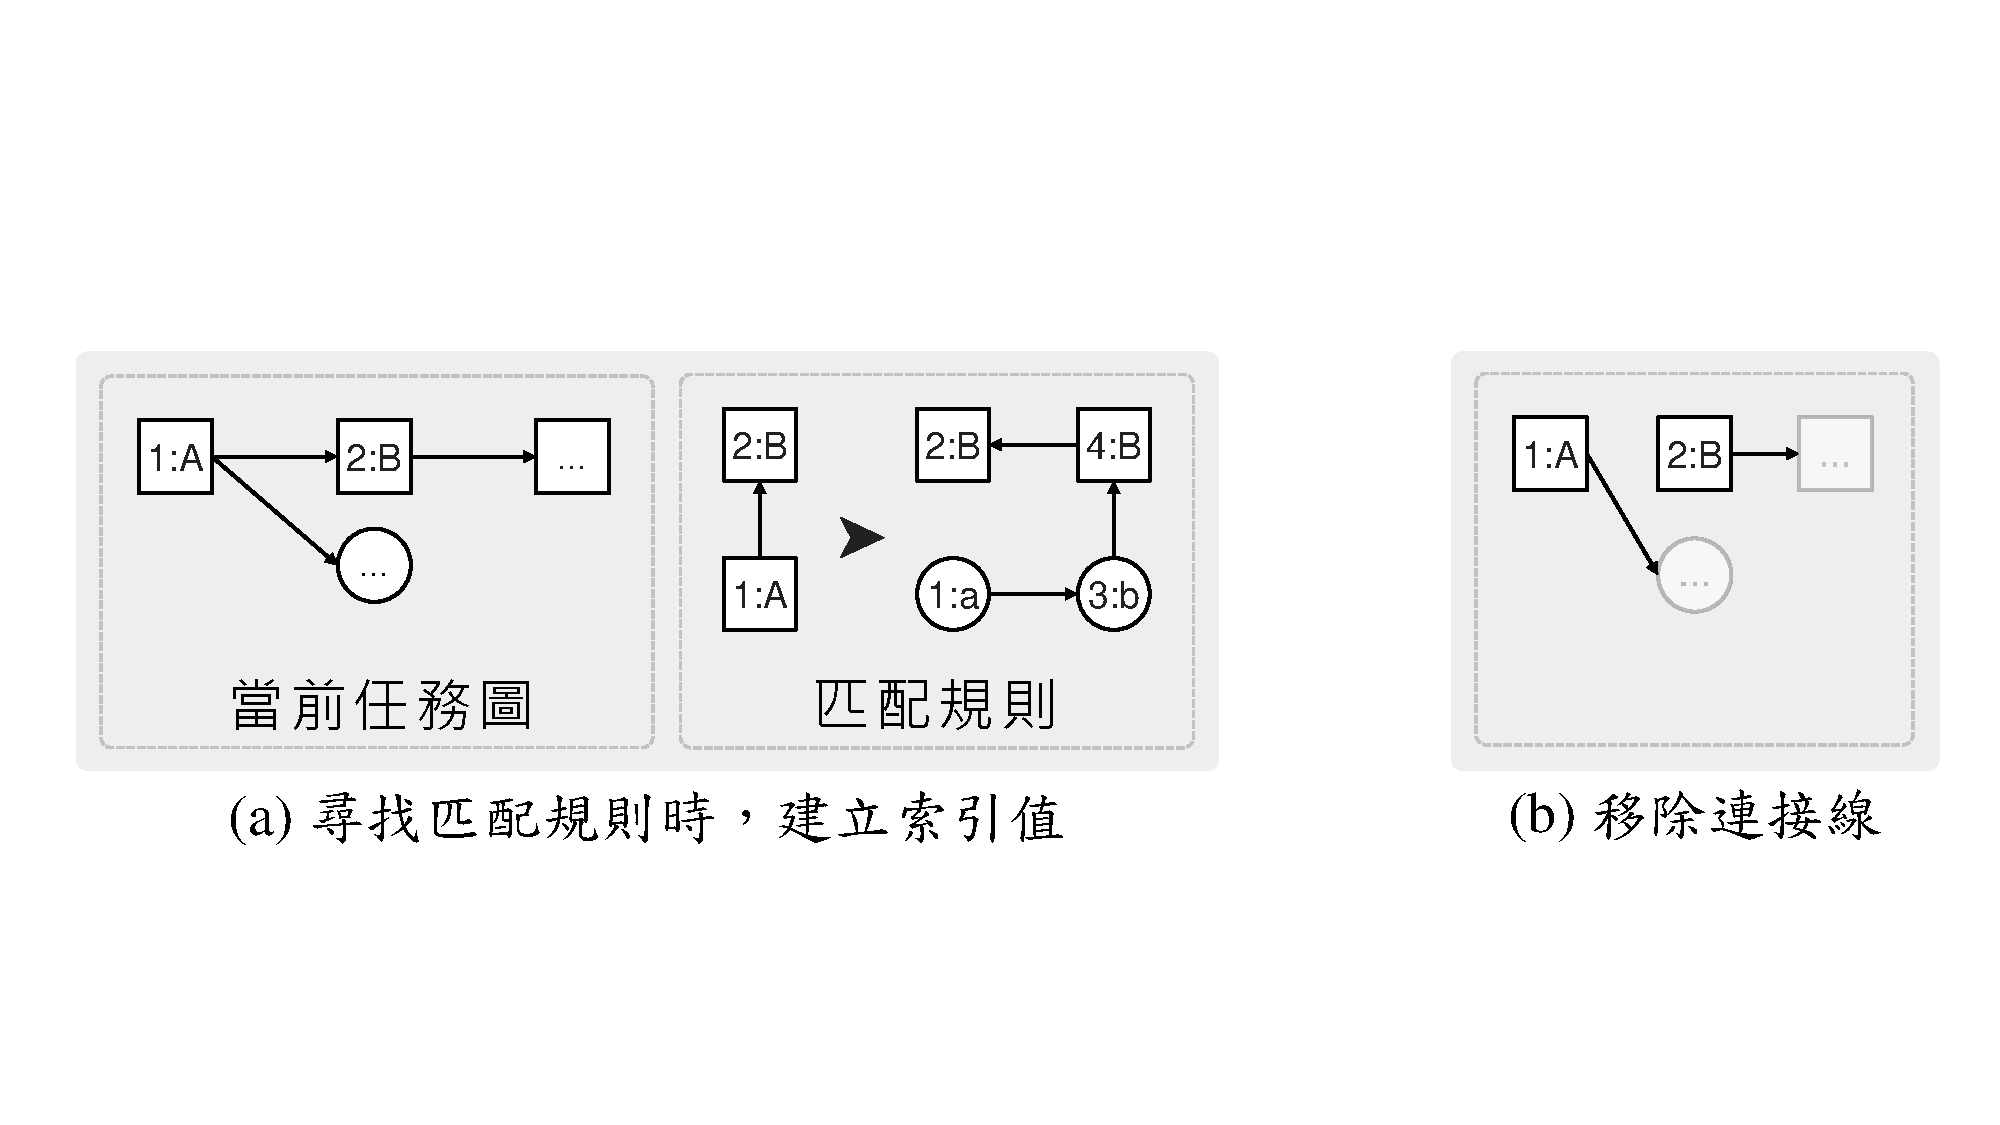
\includegraphics[width=1.0\textwidth]{figures/rewrite-system-i-flow.pdf}
    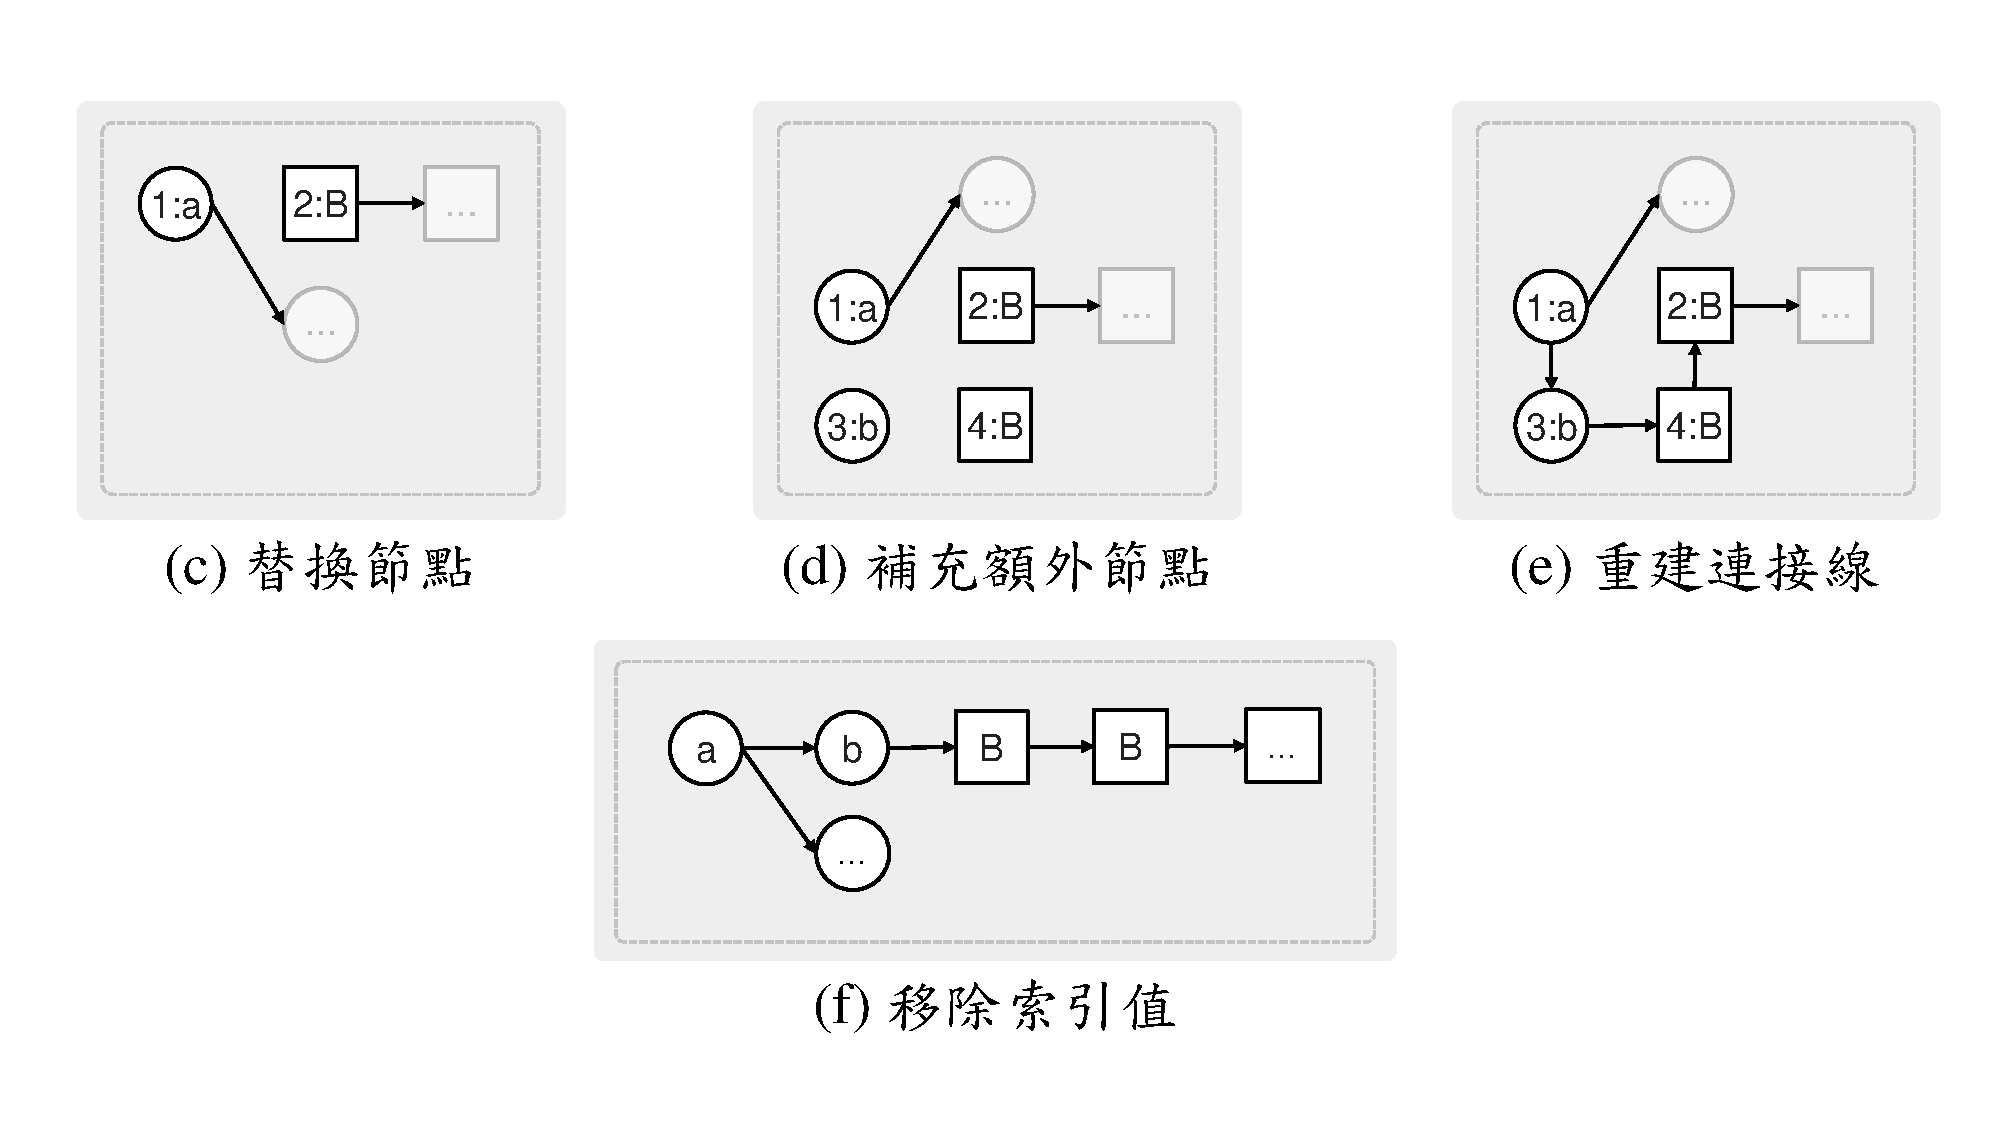
\includegraphics[width=1.0\textwidth]{figures/rewrite-system-i-flow-.pdf}
    \caption{任務語法之改寫系統流程}
    \label{fig:rewrite-system-i-flow}
  \end{center}
\end{figure}

在~\ref{ssec:method-missiongrammars-rules} 小節提及,完整的任務圖必不包含任何的非終端節點,倘若經過多次疊代改寫仍有非終端節點存在,關卡設計師必須修改任務語法其規則,使之能夠完整轉換成全終端節點的任務圖,方可進入下一階段的空間轉換。

\begin{algorithm}[!htb]
    \caption{改寫系統(任務語法)}
    \label{alg:algorithm-missiongrammars-rewritesystem}
    \begin{algorithmic}[1]
        \Require
            \Statex $root$ is current $pointer$ in the mission graph.
            \Statex $rules$ is a rule set of mission grammars.             \Comment{已過濾非法規則,篩選次數仍餘者}
            \Statex $seed$ is the random seed.
        \Ensure
            \State {Initialize random number generator via $seed$}         \Comment{初始化亂數表,如 C 的 srand}
            \Statex
            \Function{RewriteSystem1}{$root$, $rules$}
                \State {$mRule$ = FindMatchs($root$, $rules$)}             \Comment{演算法~\ref{alg:algorithm-matchedrule} 之方法,尋找匹配規則}
                \If {$mRule$ is found from $root$ and $root$ doesn't be explored}
                    \State {RemoveConnections($root$, $mRule$)}            \Comment{圖~\ref{fig:rewrite-system-i-flow} b,移除連接線}
                    \State {ReplaceNodes($root$, $mRule$)}                 \Comment{圖~\ref{fig:rewrite-system-i-flow} c,替換等價節點}
                    \State {AppendNodes($root$, $mRule$)}                  \Comment{圖~\ref{fig:rewrite-system-i-flow} d,補充額外節點}
                    \State {ReAddConnections($root$, $mRule$)}             \Comment{圖~\ref{fig:rewrite-system-i-flow} e,重建連接線}
                    \State {RevokeIndexes($root$, $mRule$)}                \Comment{圖~\ref{fig:rewrite-system-i-flow} f,移除索引值}
                \EndIf
                \ForAll {$child\in children$ of $root$}:
                    \State {RewriteSystem1($child$, $rules$)}              \Comment{遞迴式,跳往 Line $2$}
                \EndFor
                \State {\Return {$root$}}
            \EndFunction
    \end{algorithmic}
\end{algorithm}

\begin{algorithm}[!htb]
    \caption{搜尋匹配規則}
    \label{alg:algorithm-matchedrule}
    \begin{algorithmic}[1]
        \Require
            \Statex $root$ is current $pointer$ in the mission graph.
            \Statex $rules$ is a rule set of mission grammars.
        \Ensure
            \Function{FindMatchs}{$root$, $rules$}
                \State {$mRules$ is an empty array of $rule$}
                \State {$graph$ = TransformToGraph($root$)}               \Comment{以該節點作為新圖之根}
                \ForAll {$rule\in$ $rules$}:                              \Comment{參照任務規則表,表~\ref{tbl:missiongrammars-rules-linear-example}-~\ref{tbl:missiongrammars-rules-nonlinear-example3}}
                    \If {$graph$ is isomorphic with $left$ of $rule$}     \Comment{若當前圖與該規則同構}
                        \State {$mRules$ add $rule$}                      \Comment{將該規則加入候選名單}
                    \EndIf
                \EndFor
                \State {$sRule$ = RouletteWheel($mRules$)}                \Comment{採輪盤法並受演算法~\ref{alg:algorithm-missiongrammars-rewritesystem} Line $1$ 影響}
                \State {SetIndexes($root$, $sRule$)}                      \Comment{圖~\ref{fig:rewrite-system-i-flow} a,設定索引值}
                \State {\Return {$sRule$}}
            \EndFunction
    \end{algorithmic}
\end{algorithm}

圖~\ref{fig:mission-graph-generating-progress} 根據任務規則表(表~\ref{tbl:missiongrammars-rules-linear-example}-~\ref{tbl:missiongrammars-rules-nonlinear-example3})生成任務圖,並使用亂數種子 $894730$ 作舉例,每次的疊代生成依照演算法~\ref{alg:algorithm-missiongrammars-rewritesystem} 將當前任務圖的所有節點遍歷 (traversal)。根據前述章節定義,當圖~\ref{fig:mission-graph-generating-progress} d 時已不存在非終端節點,任務圖已趨穩定,但因為鎖向前規則與房間攤平規則,其規則左側皆為終端節點的情形下,儘管任務圖已趨穩定,只要任務圖中仍有同構子圖存在,改寫系統便能持續運行下去。在 \textit{Dungeon Generator} 中,亂數種子會同時決定一隨機次數,讓已趨穩定的任務圖仍能夠在有限次數下持續進行疊代,直至無任何規則可以被採用,見圖~\ref{fig:mission-graph-generating-progress} g。在圖~\ref{fig:final-mission-graph} 中展示了根據不同亂數種子,能夠得到豐富結果的任務圖。

\begin{figure}[!htb]
  \begin{center}
    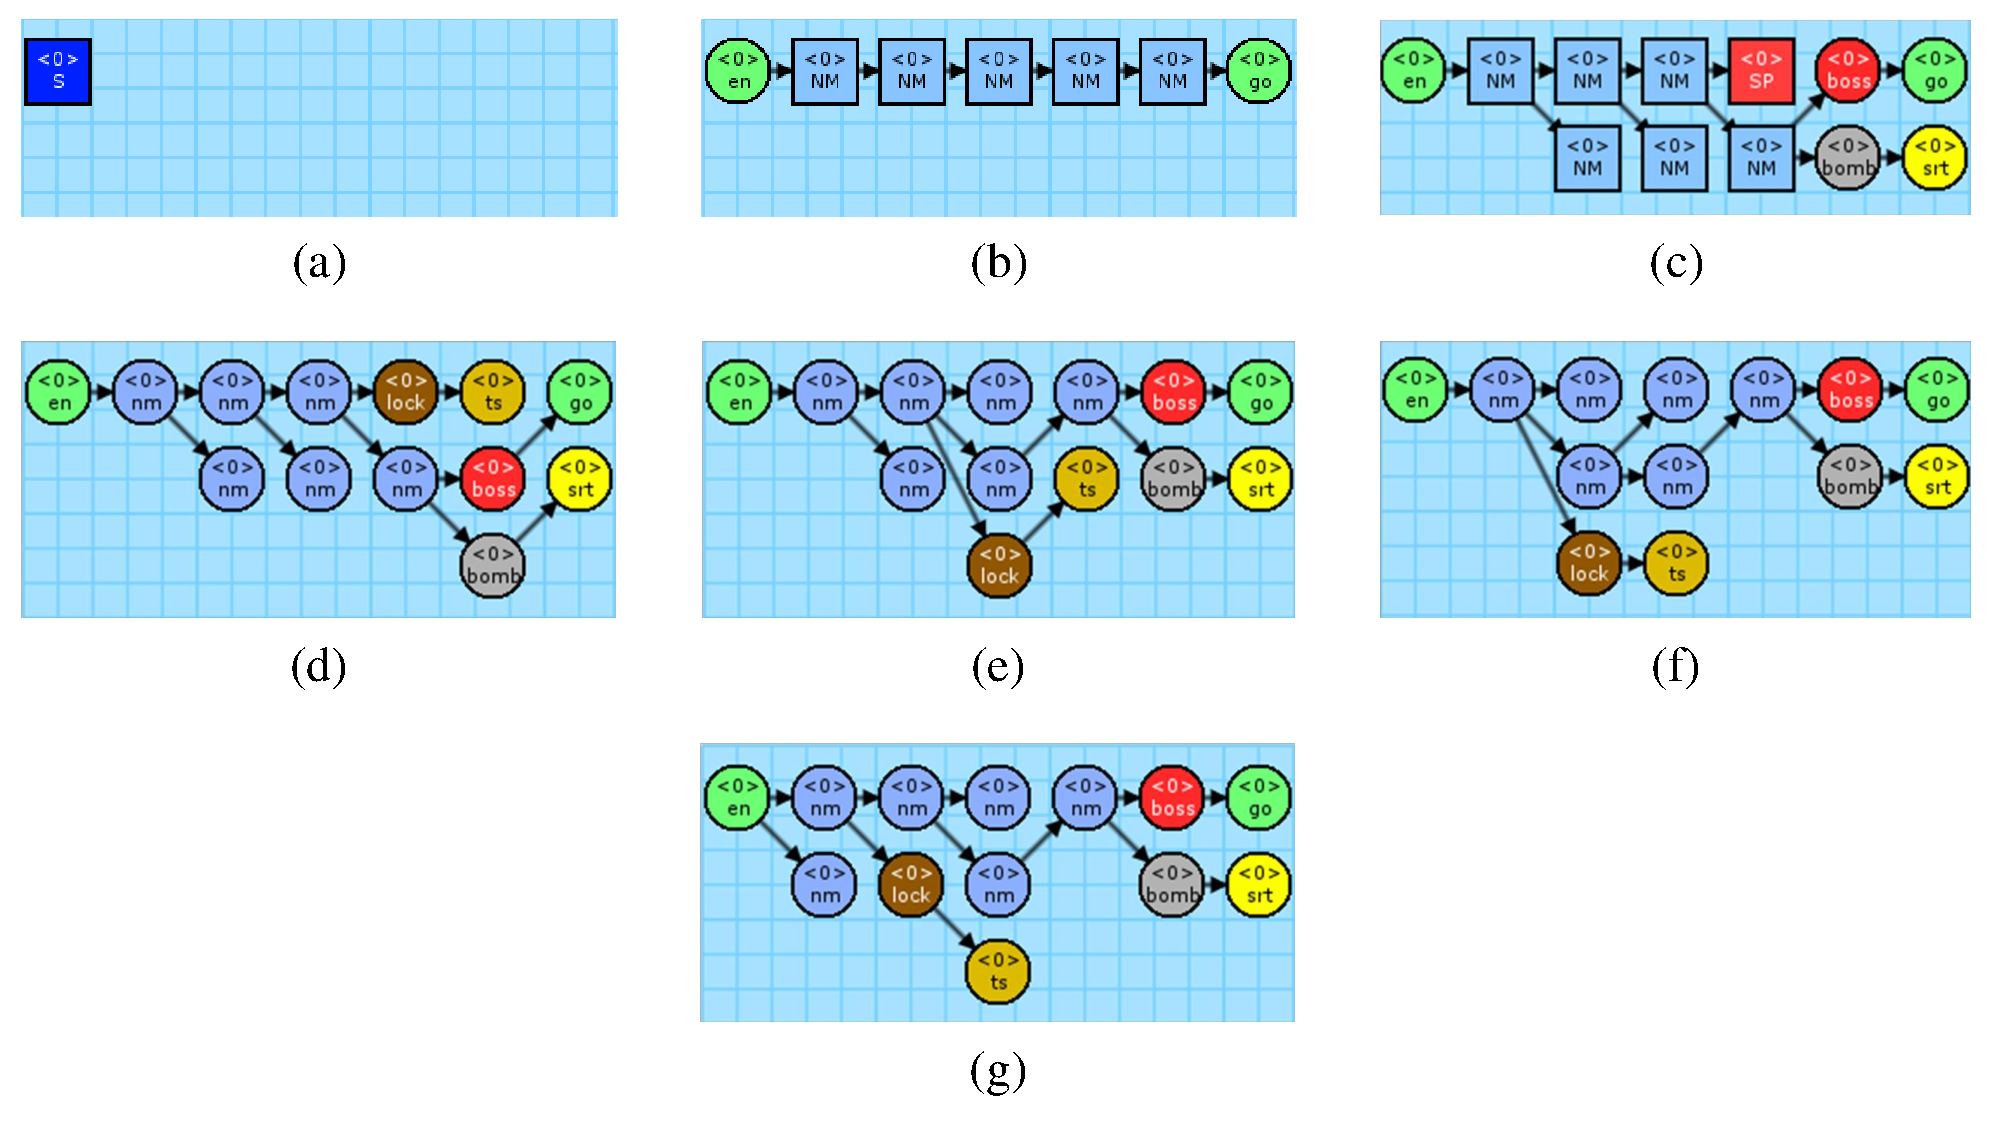
\includegraphics[width=1.0\textwidth]{figures/mission-graph-generating-progress.pdf}
    \caption{任務圖的生成過程}
    \label{fig:mission-graph-generating-progress}
  \end{center}
\end{figure}

\begin{figure}[!htb]
  \begin{center}
    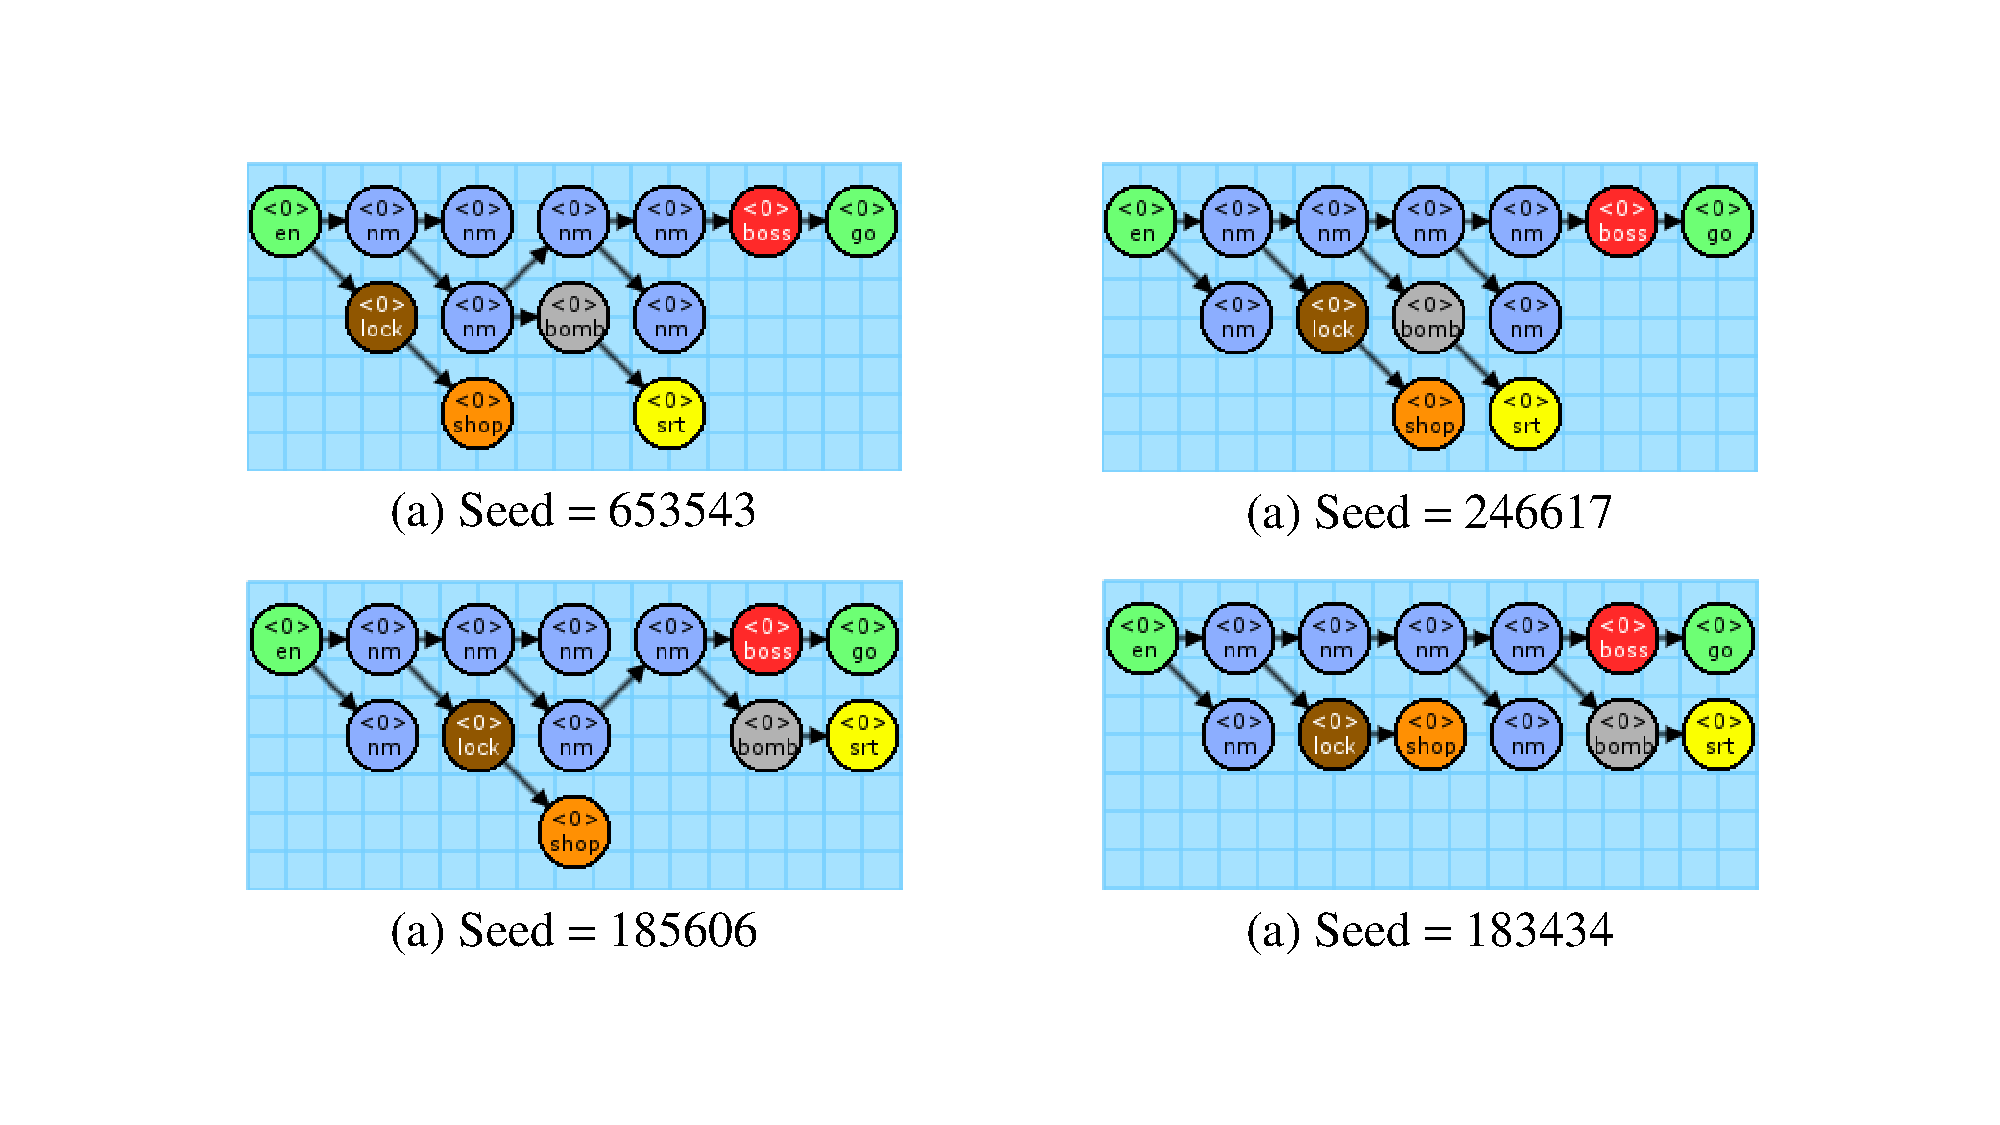
\includegraphics[width=1.0\textwidth]{figures/final-mission-graph.pdf}
    \caption{根據不同亂數種子所輸出的任務圖}
    \label{fig:final-mission-graph}
  \end{center}
\end{figure}

% Clean the page after this section.
\clearpage

\section{空間建構}
\label{sec:method-spacepieces}

Joris Dormans 於文獻中提到為二維空間的範例~\cite{dormans2010adventures}~\cite{dormans2012engineering},我們的實驗環境以三維空間為主。在空間語法中將直接構築遊戲的基礎房型,但不設置怪物、寶箱或陷阱足以直接影響遊戲性的遊戲物件,如圖~\ref{fig:gameobject-list}。此外,我們希望空間中的遊戲物件能夠有意義的自動化配置,即在設計空間語法的流程中,忽略絕大部分的遊戲物件配置,直到~\ref{sec:method-segments} 節提出之方法達成。

\begin{figure}[!htb]
  \begin{center}
    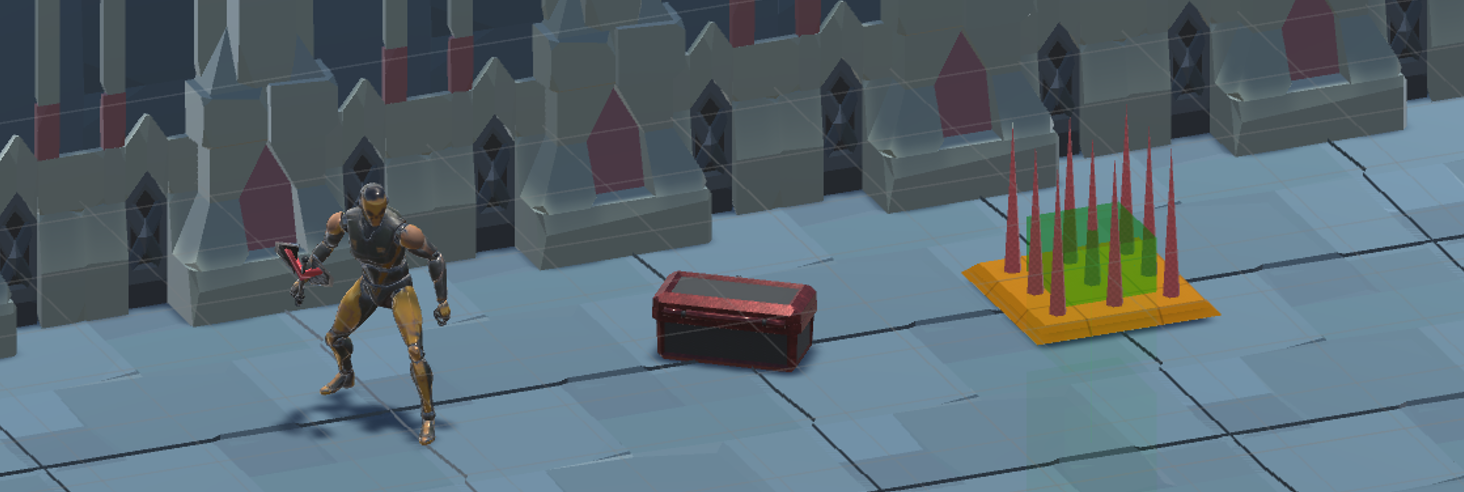
\includegraphics[width=1.0\textwidth]{figures/gameobject-list.png}
    \caption{影響遊戲性的遊戲物件,由左至右分別為敵方、寶箱與陷阱} 
    \label{fig:gameobject-list}
  \end{center}
\end{figure}

\subsection{基礎結構}
\label{ssec:method-spacepieces-basic}

我們對於空間語法做了修改以利實驗環境建置。在一個關卡 (level) 中包含數個房間容器 (volumes),每一房間容器由不定數量的房間塊 (chucks) 組成,且房間塊固定以 $9\times 9\times 9$ 個長方體體素 (voxels) 所構成,每一體素的大小為 $3\times 2\times 3$。

此外,每一個體素被分為九種方向,分別為正四方、斜四方與中心點。圖~\ref{fig:decorations-with-directions} a-c 可見,進行房間容器編輯模式下,選定一裝飾物後需透過提示色框進行位置的確認與擺放,水藍色立方體為當前體素,紅色方框為當前方位。不同的裝飾物會依照其特性決定能夠放置的方位,如地面則放置於中心點,圖~\ref{fig:decorations-with-directions} a;牆壁、階梯或門放置於正四方,圖~\ref{fig:decorations-with-directions} b;牆壁柱放置於斜四方,圖~\ref{fig:decorations-with-directions} c。在一個體素中,多個裝飾物是能夠同時並存的,例如在其放置地面、一道牆壁、兩道牆壁柱。在本次實驗環境中,我們將會使用圖~\ref{fig:decorations-with-directions} d-g 中,「地面、階梯、牆壁、牆壁柱、門」共五種裝飾物進行房間容器的體素建置工作。

\begin{figure}[!htb]
  \begin{center}
    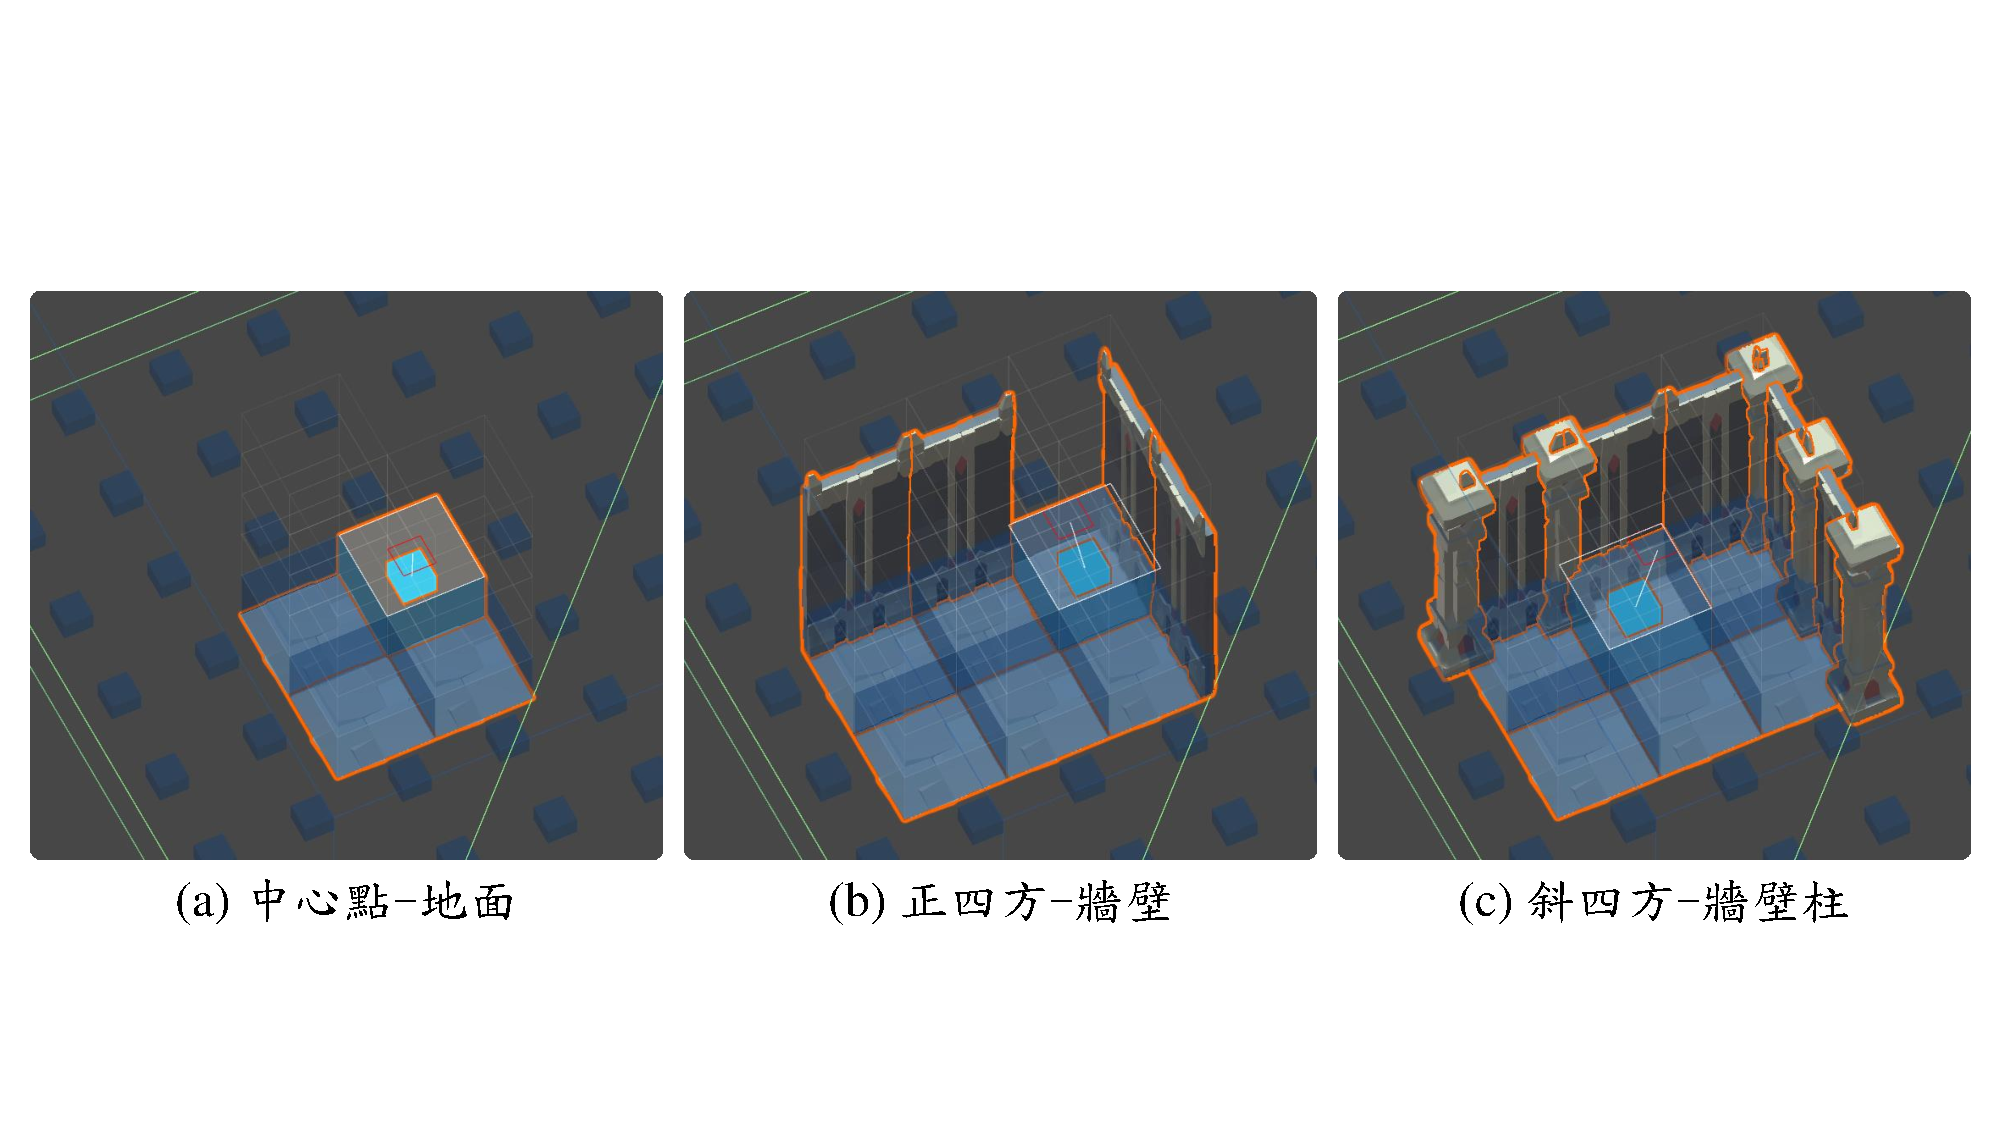
\includegraphics[width=1.0\textwidth]{figures/decorations-with-directions.pdf}
    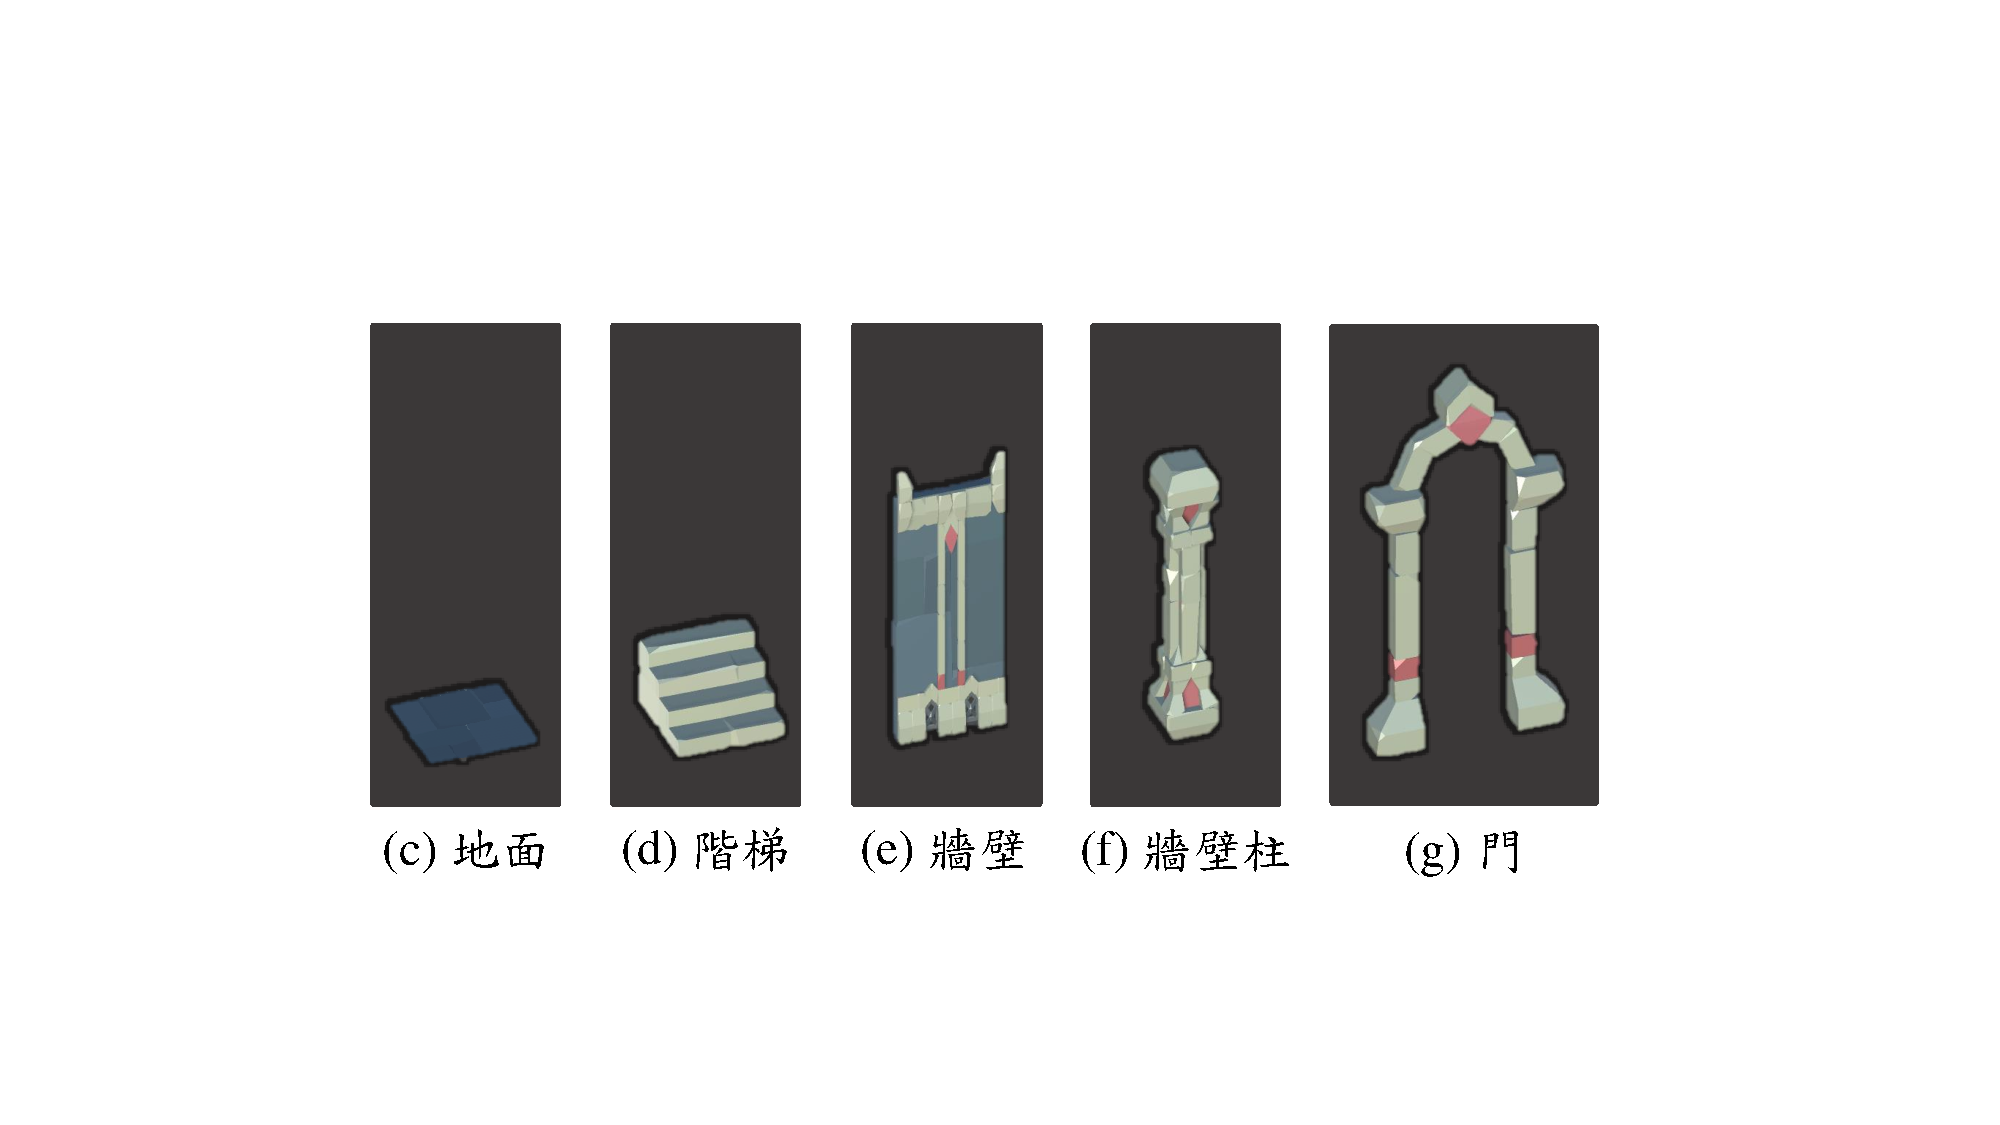
\includegraphics[width=1.0\textwidth]{figures/decorations-with-directions-.pdf}
    \caption{房間容器的體素建置方式,與五種裝飾物}
    \label{fig:decorations-with-directions}
  \end{center}
\end{figure}

\subsection{端點識別物}
\label{ssec:method-spacepieces-connections}

逐一設計出各式各樣的房間容器後,必須正確地將個空間相互連接。參考 Joris Dormans 的空間語法~\cite{dormans2012engineering},我們為體素型的房間容器添加端點識別物 (connection markers),而端點可再細分為入口 (entrance) 與出口 (exit),依照遊戲設計師需求,能夠自行擴充出口的類型,可為複數個出口識別物。在一房間容器中,最多僅能擁有一個入口識別物,而出口識別物的數量不在此限,且二者之數量總和必大於零。倘若空間當中沒有一個以上入口識別物,便會從現有的出口識別物中隨機挑選一與入口識別物相同功能執行之。圖~\ref{fig:connections-in-volume} 中描述了端點識別物的使用情境,入口的箭頭朝向空間內部,而出口的箭頭會朝向空間外部。

\begin{figure}[!htb]
  \begin{center}
    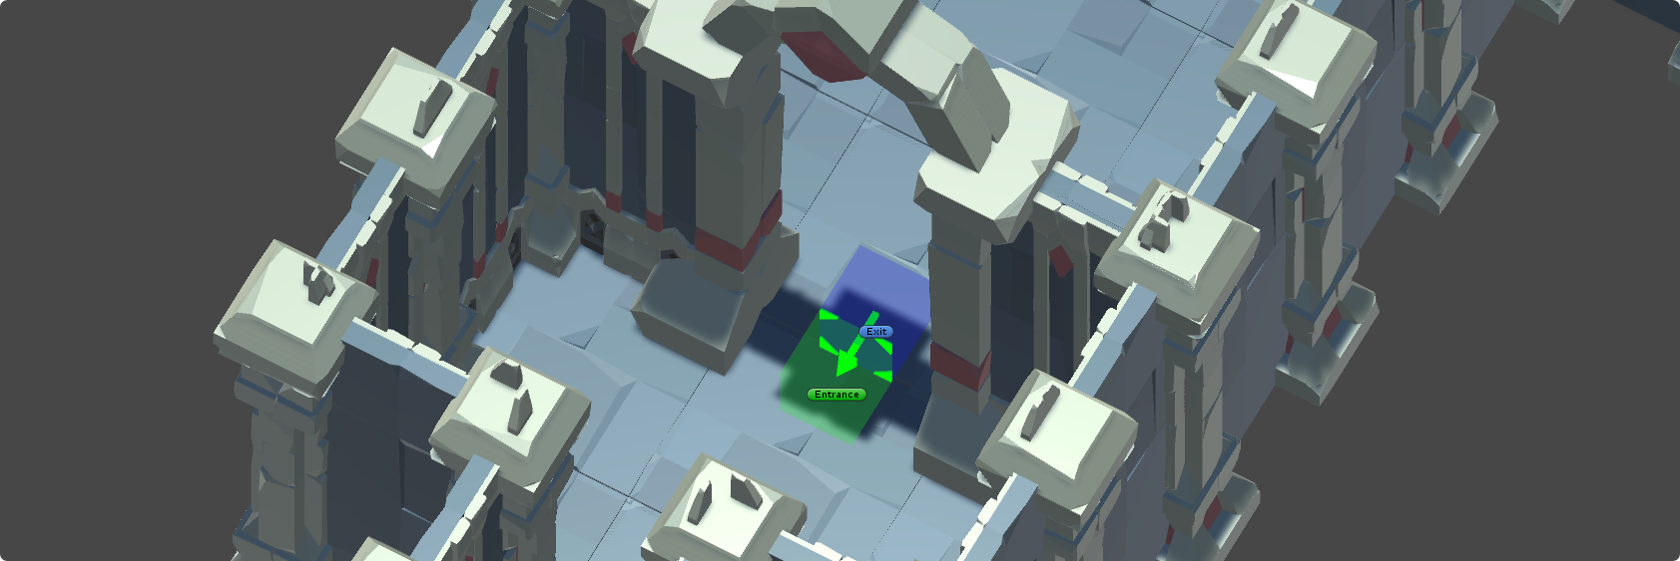
\includegraphics[width=1.0\textwidth]{figures/connections-in-volume.png}
    \caption{端點識別物的實際使用與串接情形} 
    \label{fig:connections-in-volume}
  \end{center}
\end{figure}

\subsection{房間容器類型}
\label{ssec:method-spacepieces-types}

延續第~\ref{sec:method-missiongrammars} 節任務語法所定義的任務終端節點,依照節點性質設計房型,區分出數項不同房型的空間規劃。

\subsubsection{起點、終點、魔王房}
\label{sssec:method-spacepieces-types-mainpath-i}

圖~\ref{fig:roomtype-mainpath-i} a 為起點擁有一個入口與三個出口,為玩家重生的起始房間;圖~\ref{fig:roomtype-mainpath-i} b 為終點擁有一個入口,為遊戲關卡結束的房間;圖~\ref{fig:roomtype-mainpath-i} c 為魔王房擁有一個入口與一個出口,玩家會在此房間遭遇強大敵人。

\begin{figure}[!htb]
  \begin{center}
    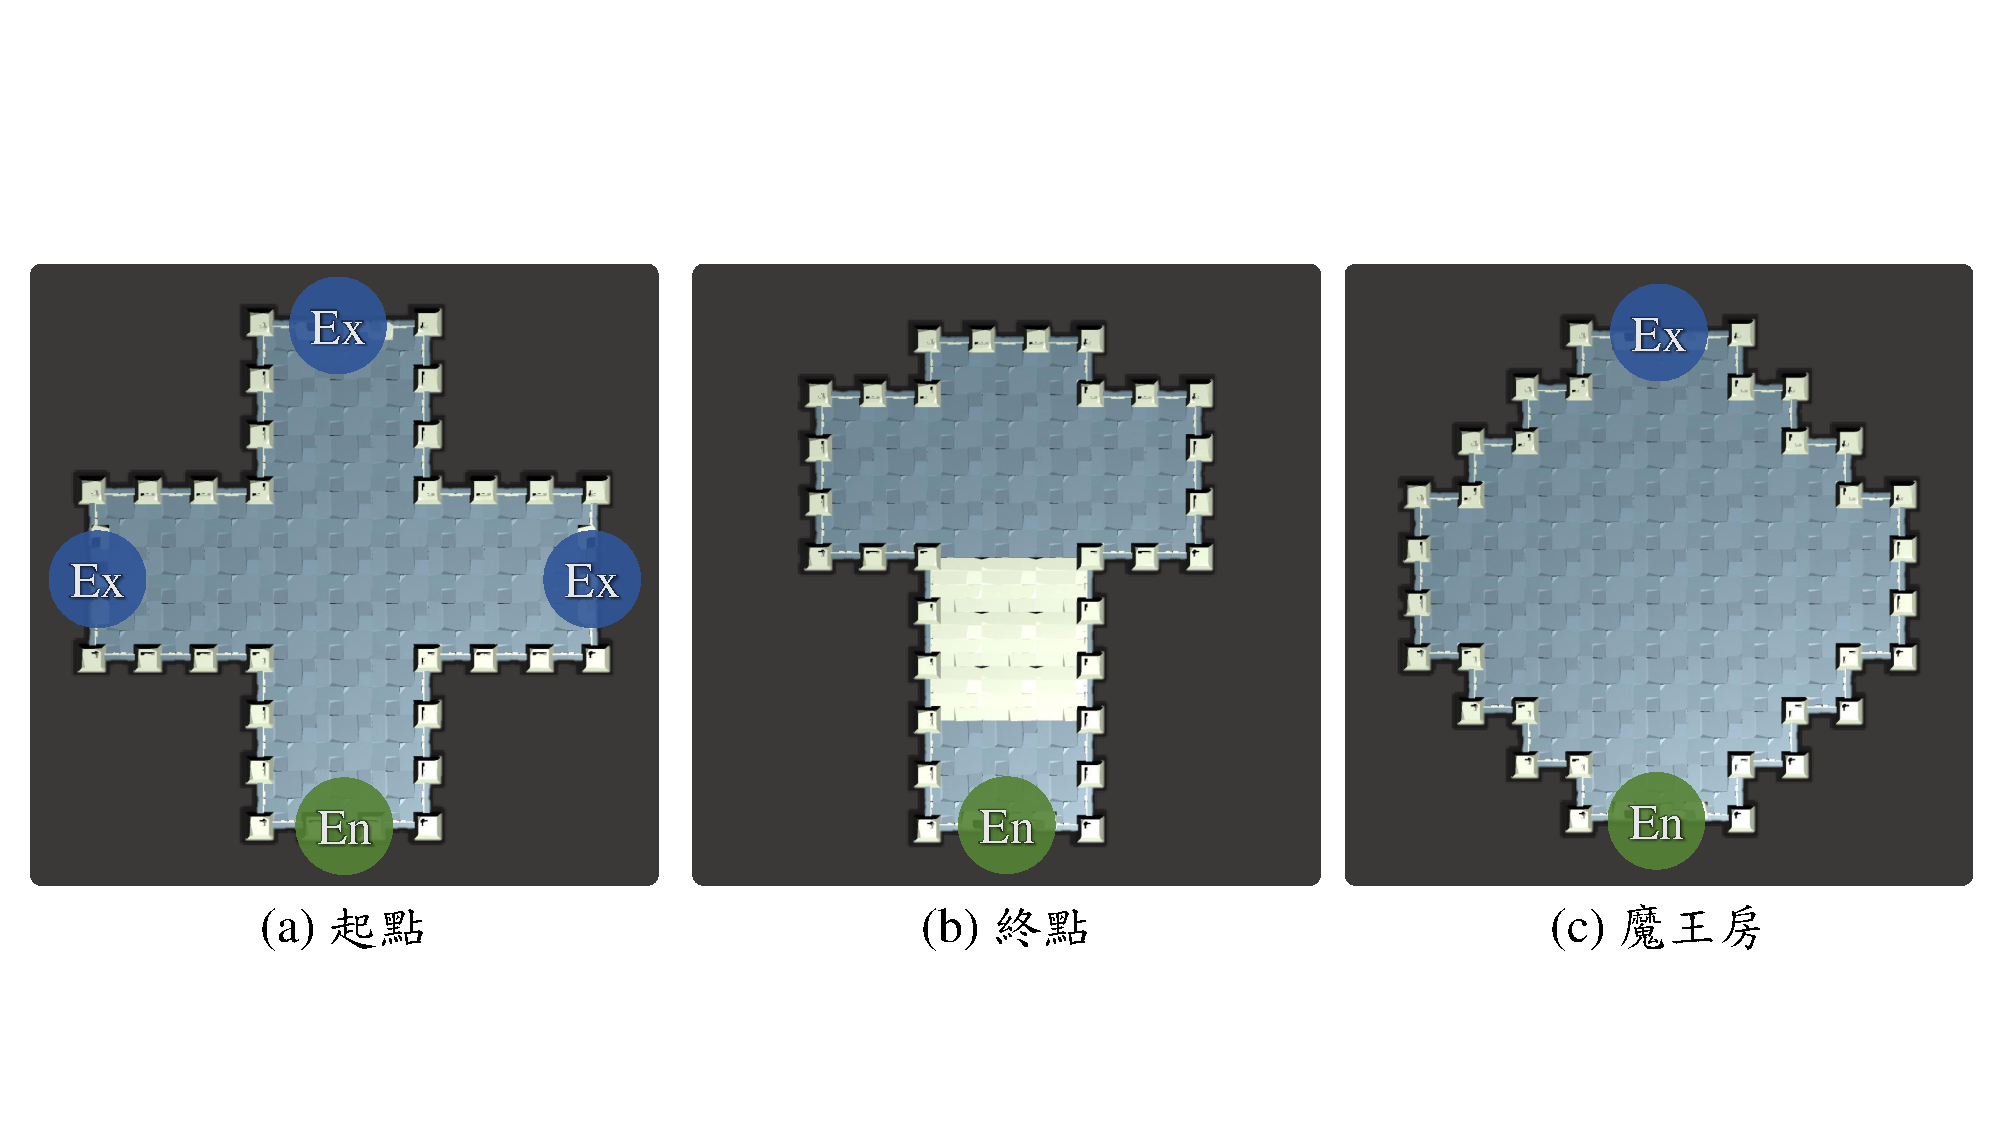
\includegraphics[width=1.0\textwidth]{figures/roomtype-mainpath-i.pdf}
    \caption{起點、終點與魔王房的房間容器結構}
    \label{fig:roomtype-mainpath-i}
  \end{center}
\end{figure}

\subsubsection{通道}
\label{sssec:method-spacepieces-types-path}

圖~\ref{fig:roomtype-mainpath-ii} 中,通道共有四種,隨著端點數量有等同的出口數量,因沒有入口識別物,便能夠以任一出口作為入口,搭配房間容器旋轉能達到共計 $11$ 種房型同構。圖~\ref{fig:roomtype-mainpath-ii} a 為 $I$ 型通道擁有二個出口,有二種同構結構;圖~\ref{fig:roomtype-mainpath-ii} b 為 $L$ 型通道擁有二個出口,有四種同構結構;圖~\ref{fig:roomtype-mainpath-ii} c 為 $T$ 型通道擁有三個出口,有四種同構結構;圖~\ref{fig:roomtype-mainpath-ii} d 為 $+$ 型通道擁有四個出口。

\begin{figure}[!htb]
  \begin{center}
    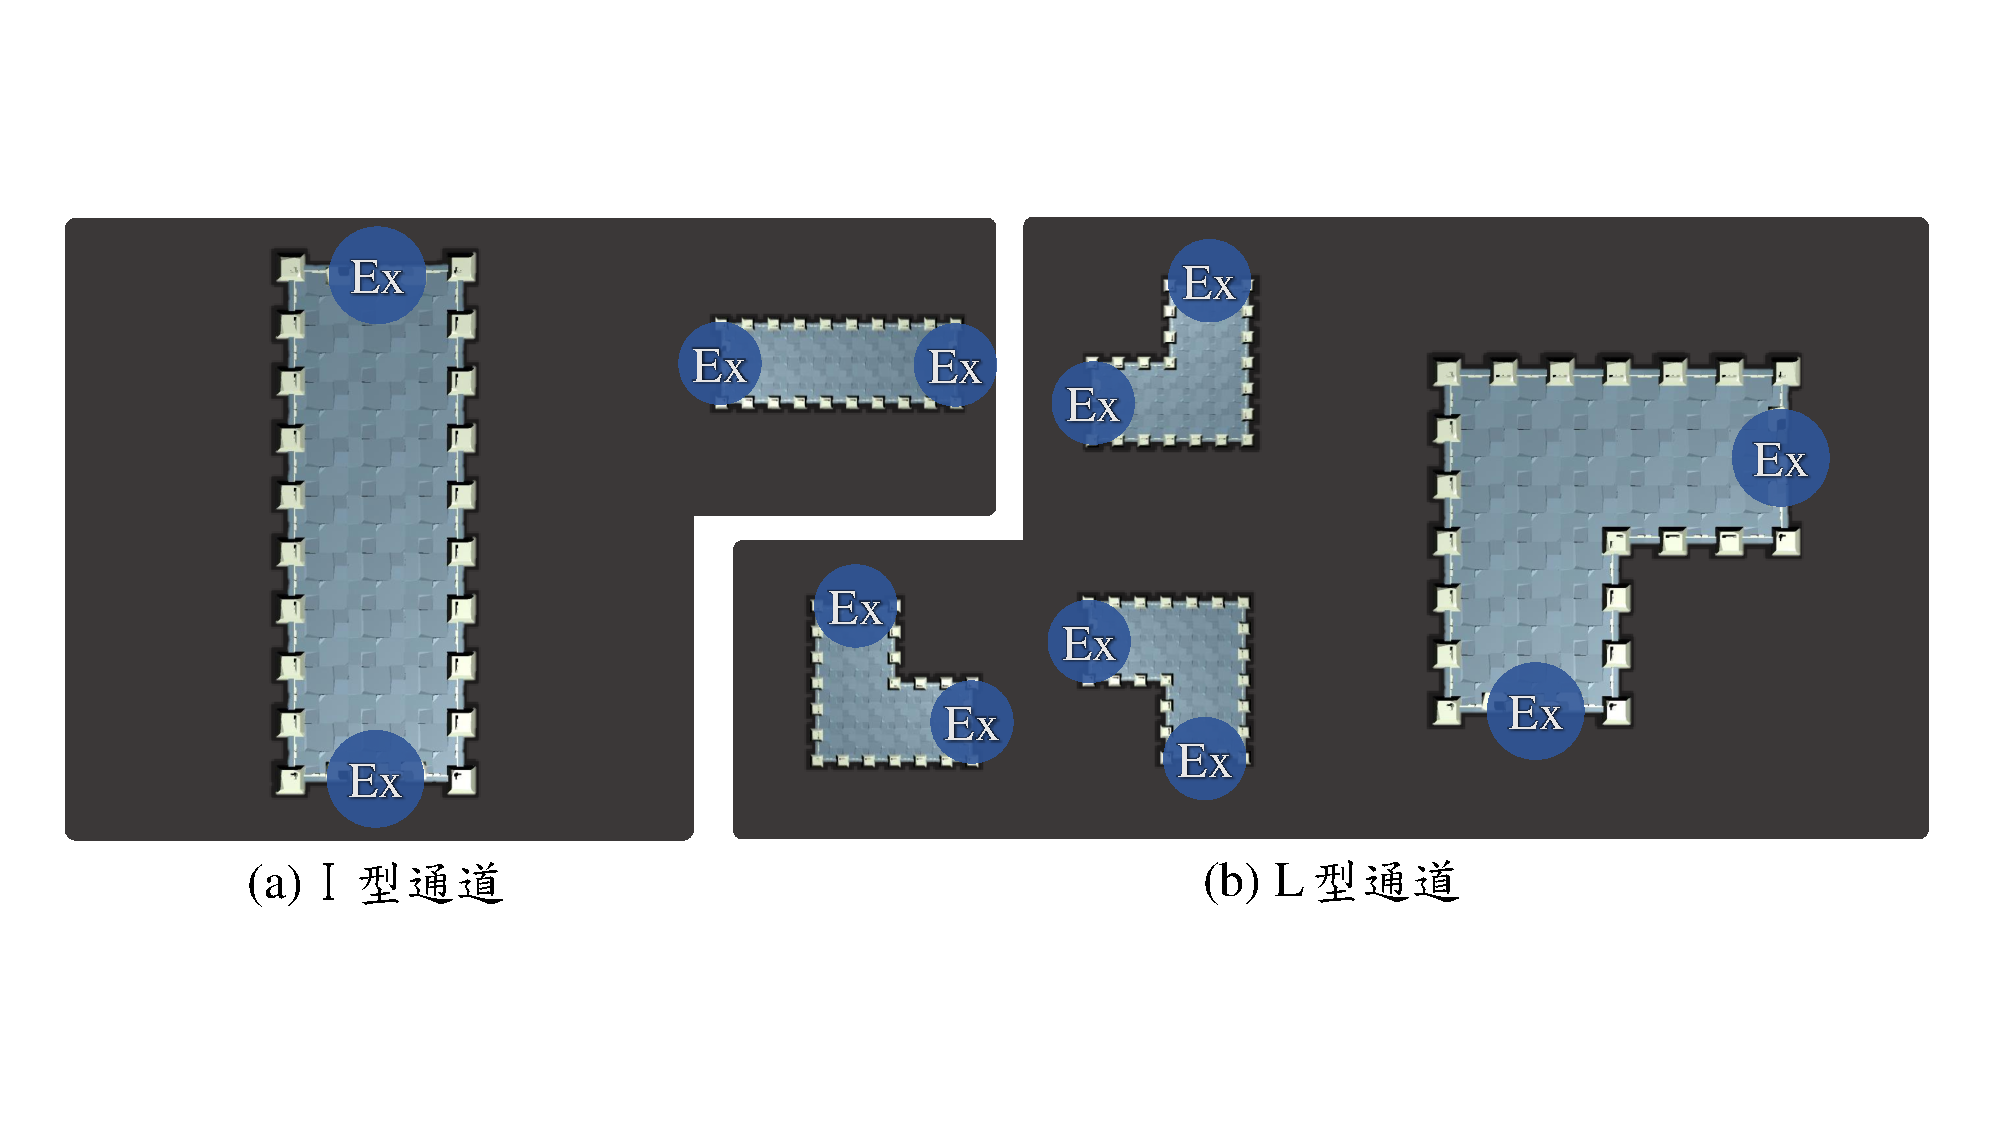
\includegraphics[width=1.0\textwidth]{figures/roomtype-mainpath-ii.pdf}
    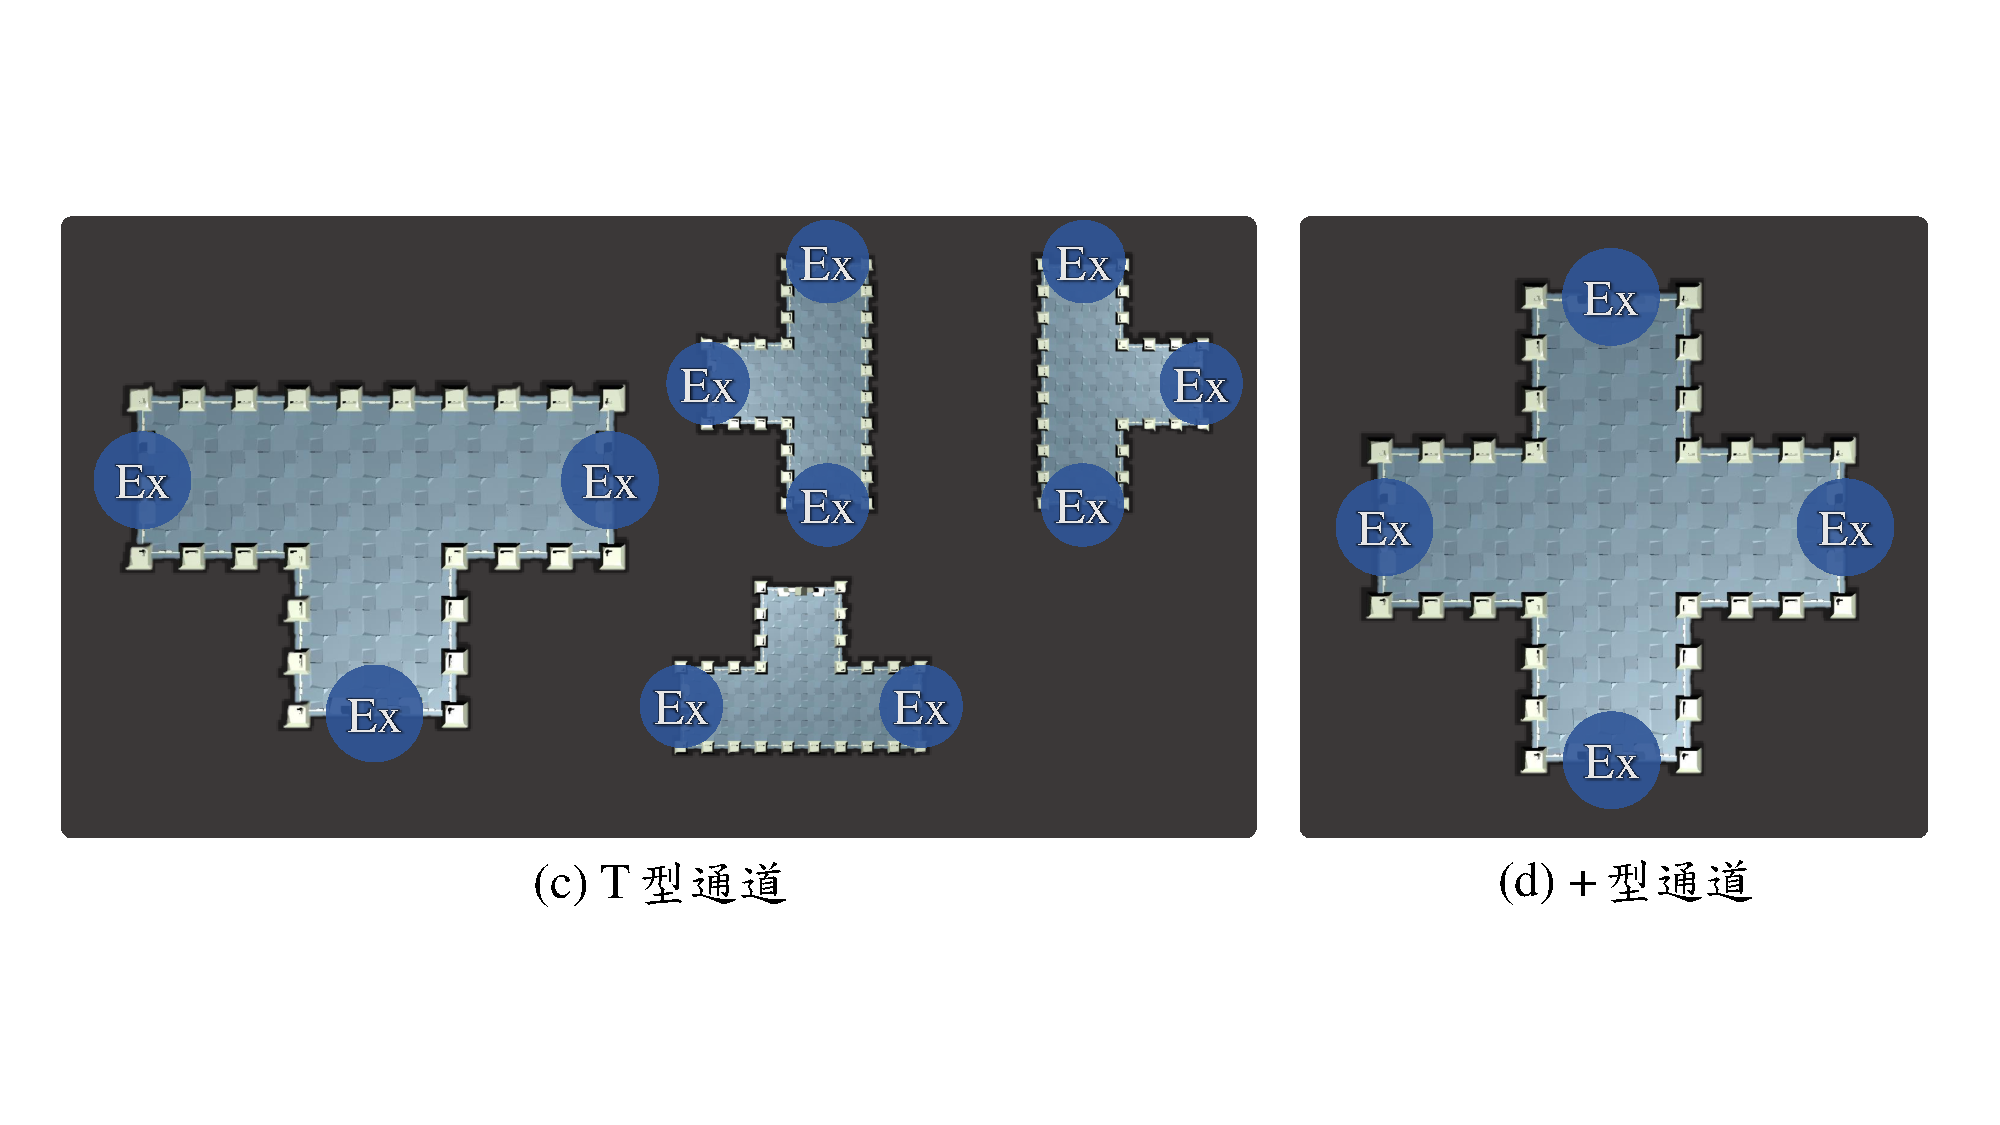
\includegraphics[width=1.0\textwidth]{figures/roomtype-mainpath-ii-.pdf}
    \caption{通道房間的房間容器結構與其同構示意}
    \label{fig:roomtype-mainpath-ii}
  \end{center}
\end{figure}

\subsubsection{石牆、秘密房、鎖、商店、寶藏房}
\label{sssec:method-spacepieces-types-special}

圖~\ref{fig:roomtype-special} a 為石牆擁有一個入口及一個出口,而出口的相同位置有石牆識別物;圖~\ref{fig:roomtype-special} b 為秘密房擁有一個入口,玩家能在該空間取得鑰匙識別物;圖~\ref{fig:roomtype-special} c 為鎖空間擁有一個入口及一個出口,在出口的相同位置有鎖識別物,玩家必須取得鑰匙方可通過;圖~\ref{fig:roomtype-special} d-e 為商店與寶藏房各擁有一個入口,玩家能夠在該房間觸發特殊事件。

\begin{figure}[!htb]
  \begin{center}
    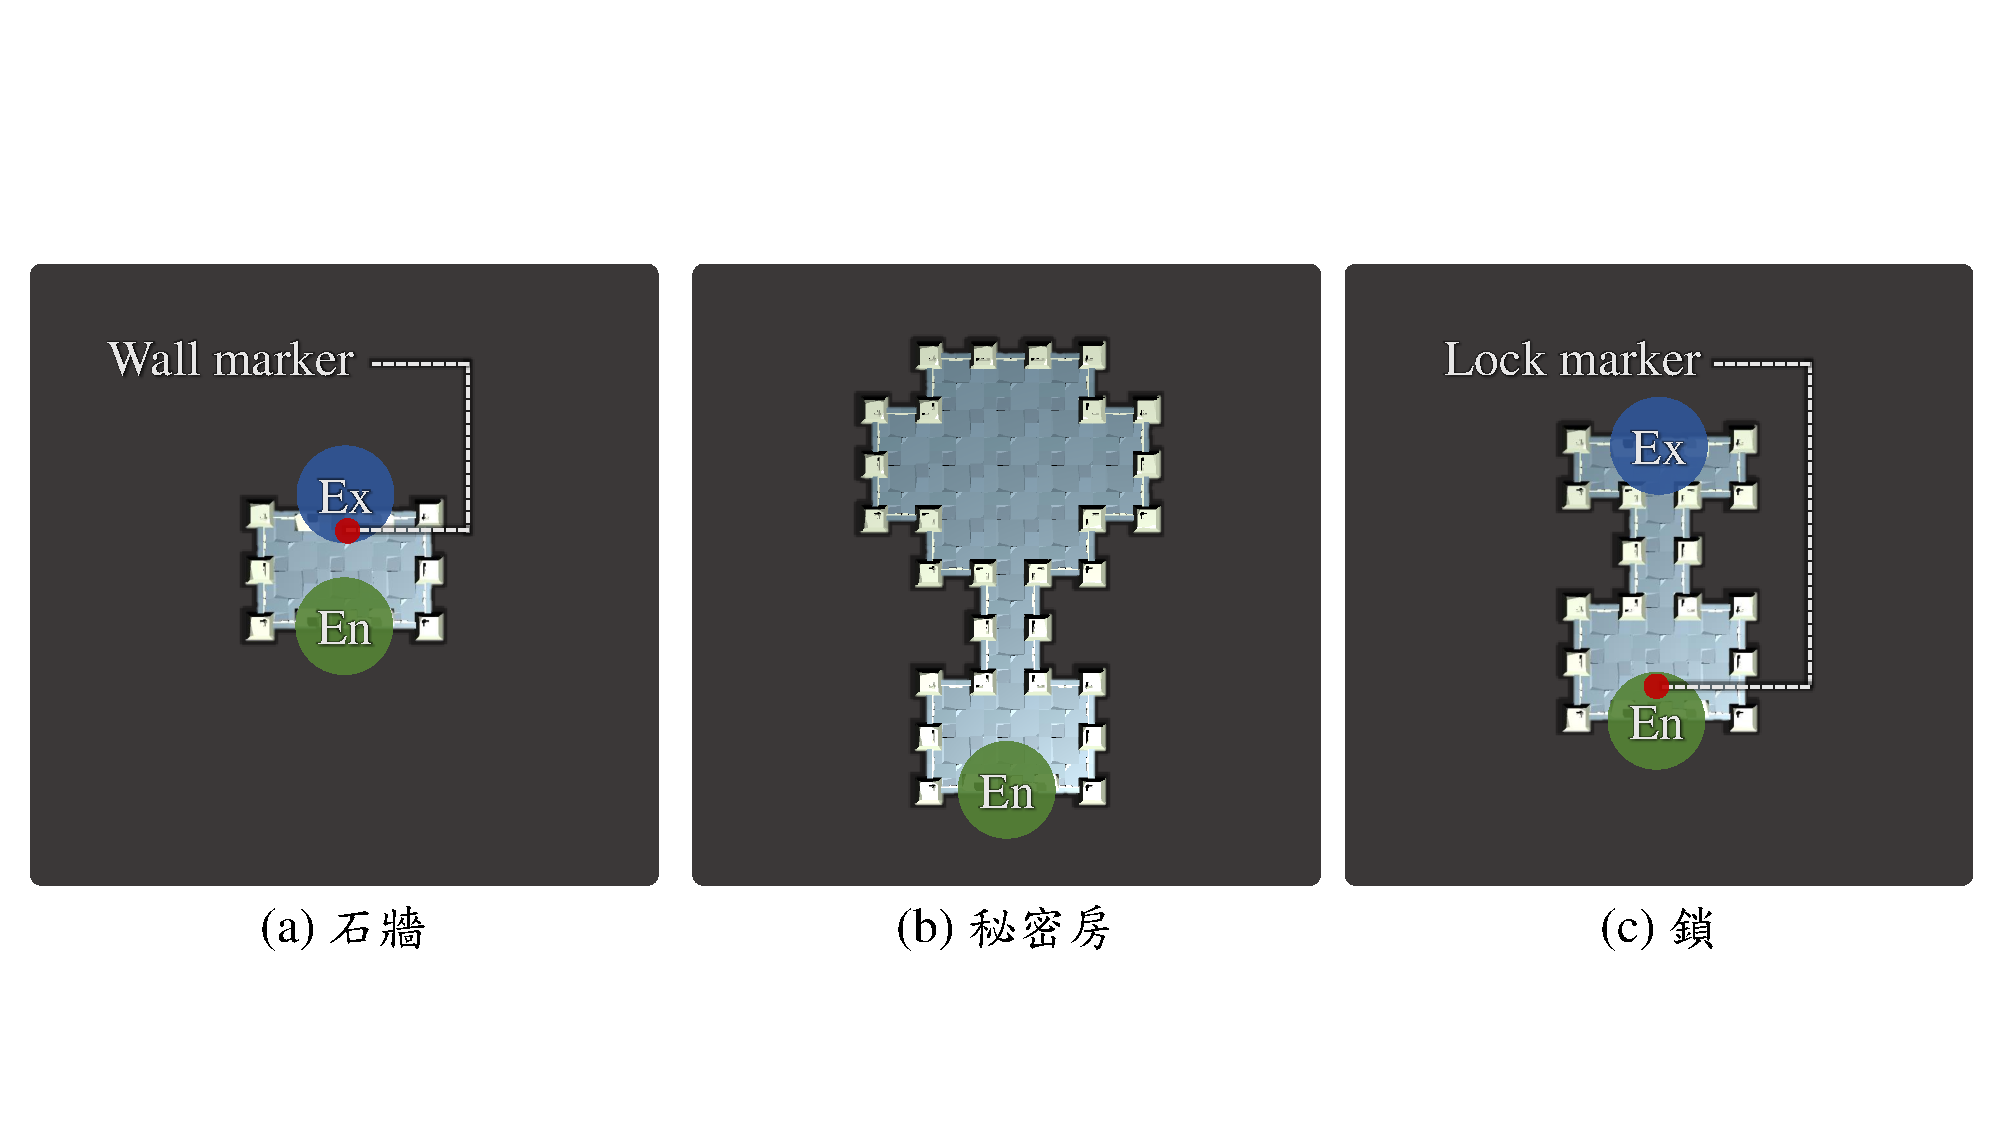
\includegraphics[width=1.0\textwidth]{figures/roomtype-special.pdf}
    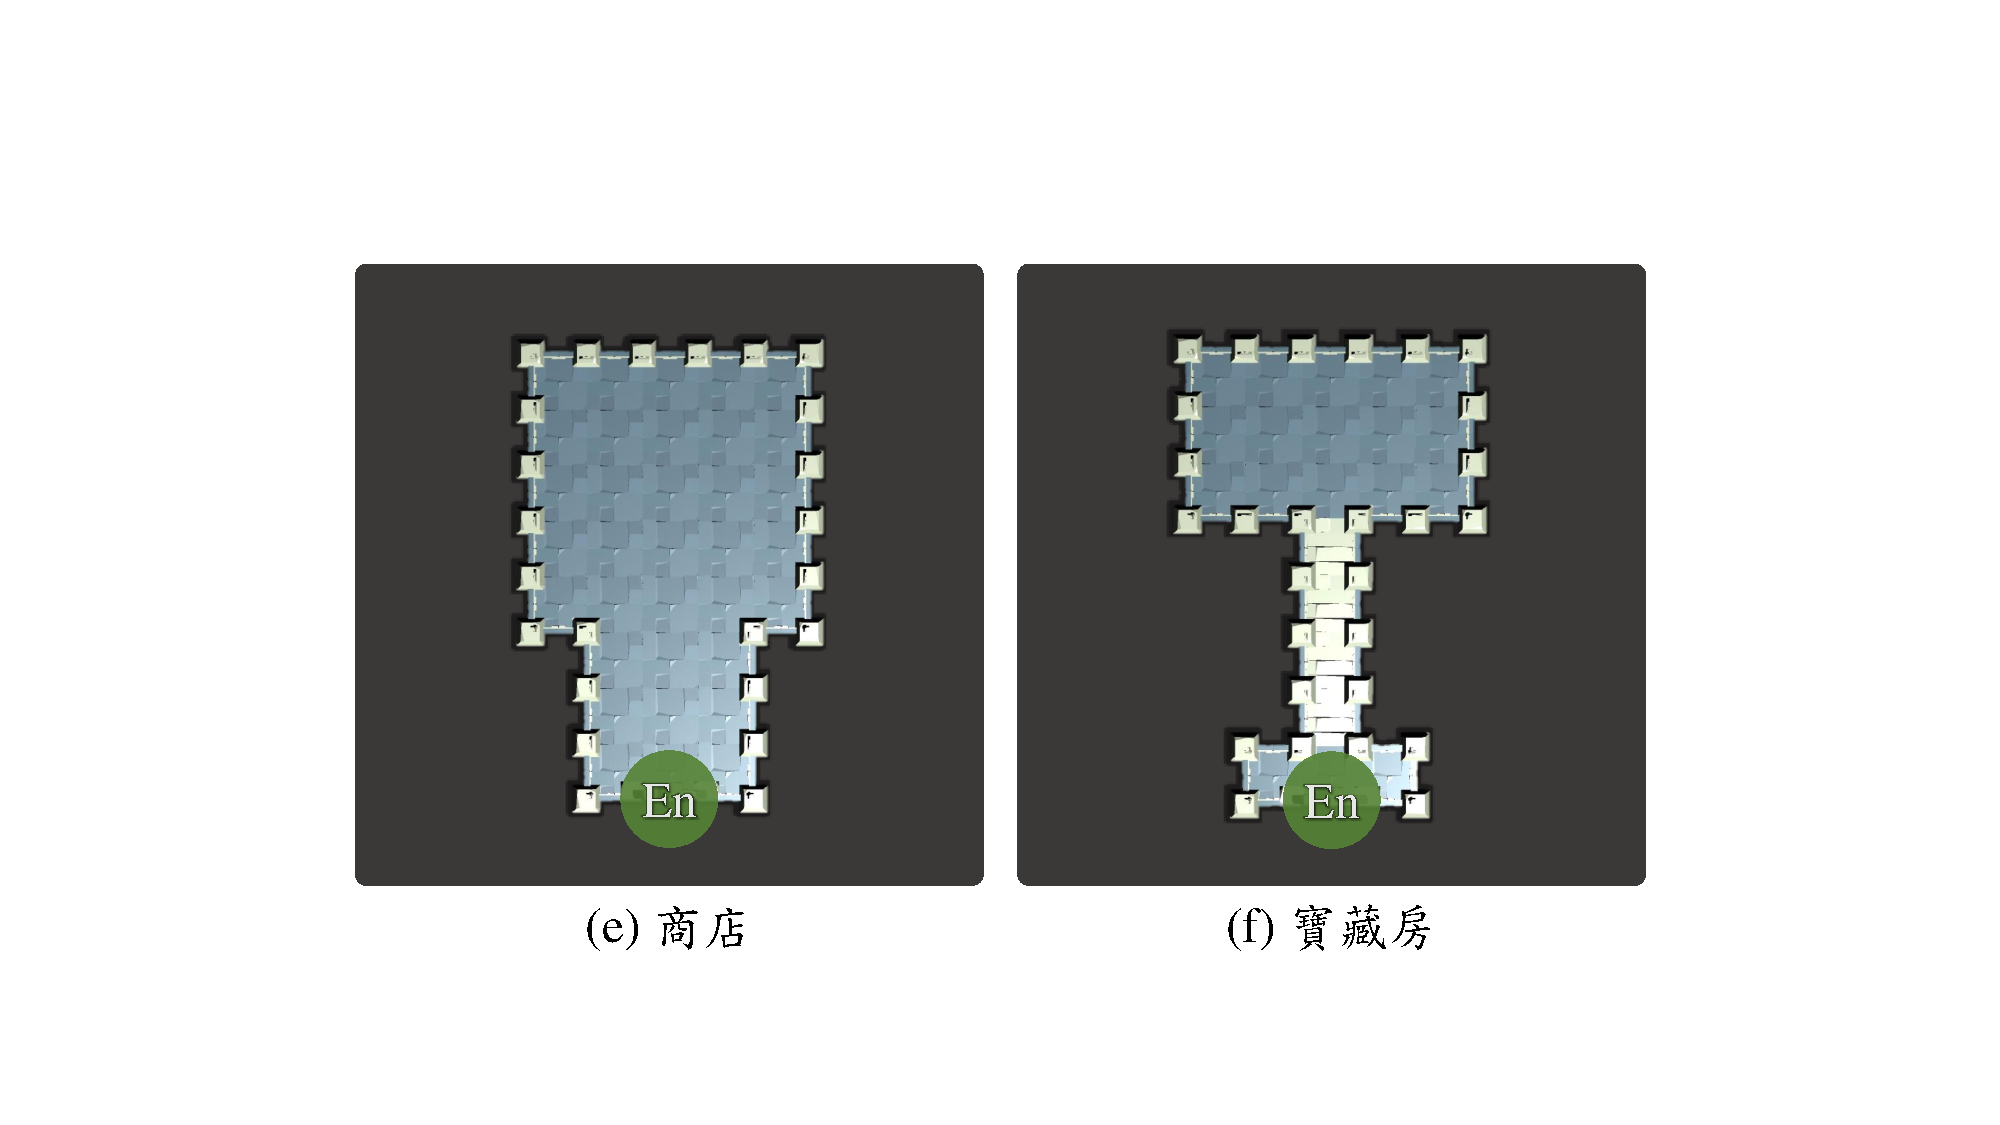
\includegraphics[width=1.0\textwidth]{figures/roomtype-special-.pdf}
    \caption{石牆、秘密房、鎖、商店與寶藏房的房間容器結構}
    \label{fig:roomtype-special}
  \end{center}
\end{figure}

\subsubsection{死路}
\label{sssec:method-spacepieces-types-wall}

在第~\ref{ssec:method-spacepieces-frommissiontospace} 小節中,為了要封閉剩餘的端點識別物所造成的空間開口,便需要無特殊功能的單一入口空間容器,見圖~\ref{fig:roomtype-wall}。

\begin{figure}[!htb]
  \begin{center}
    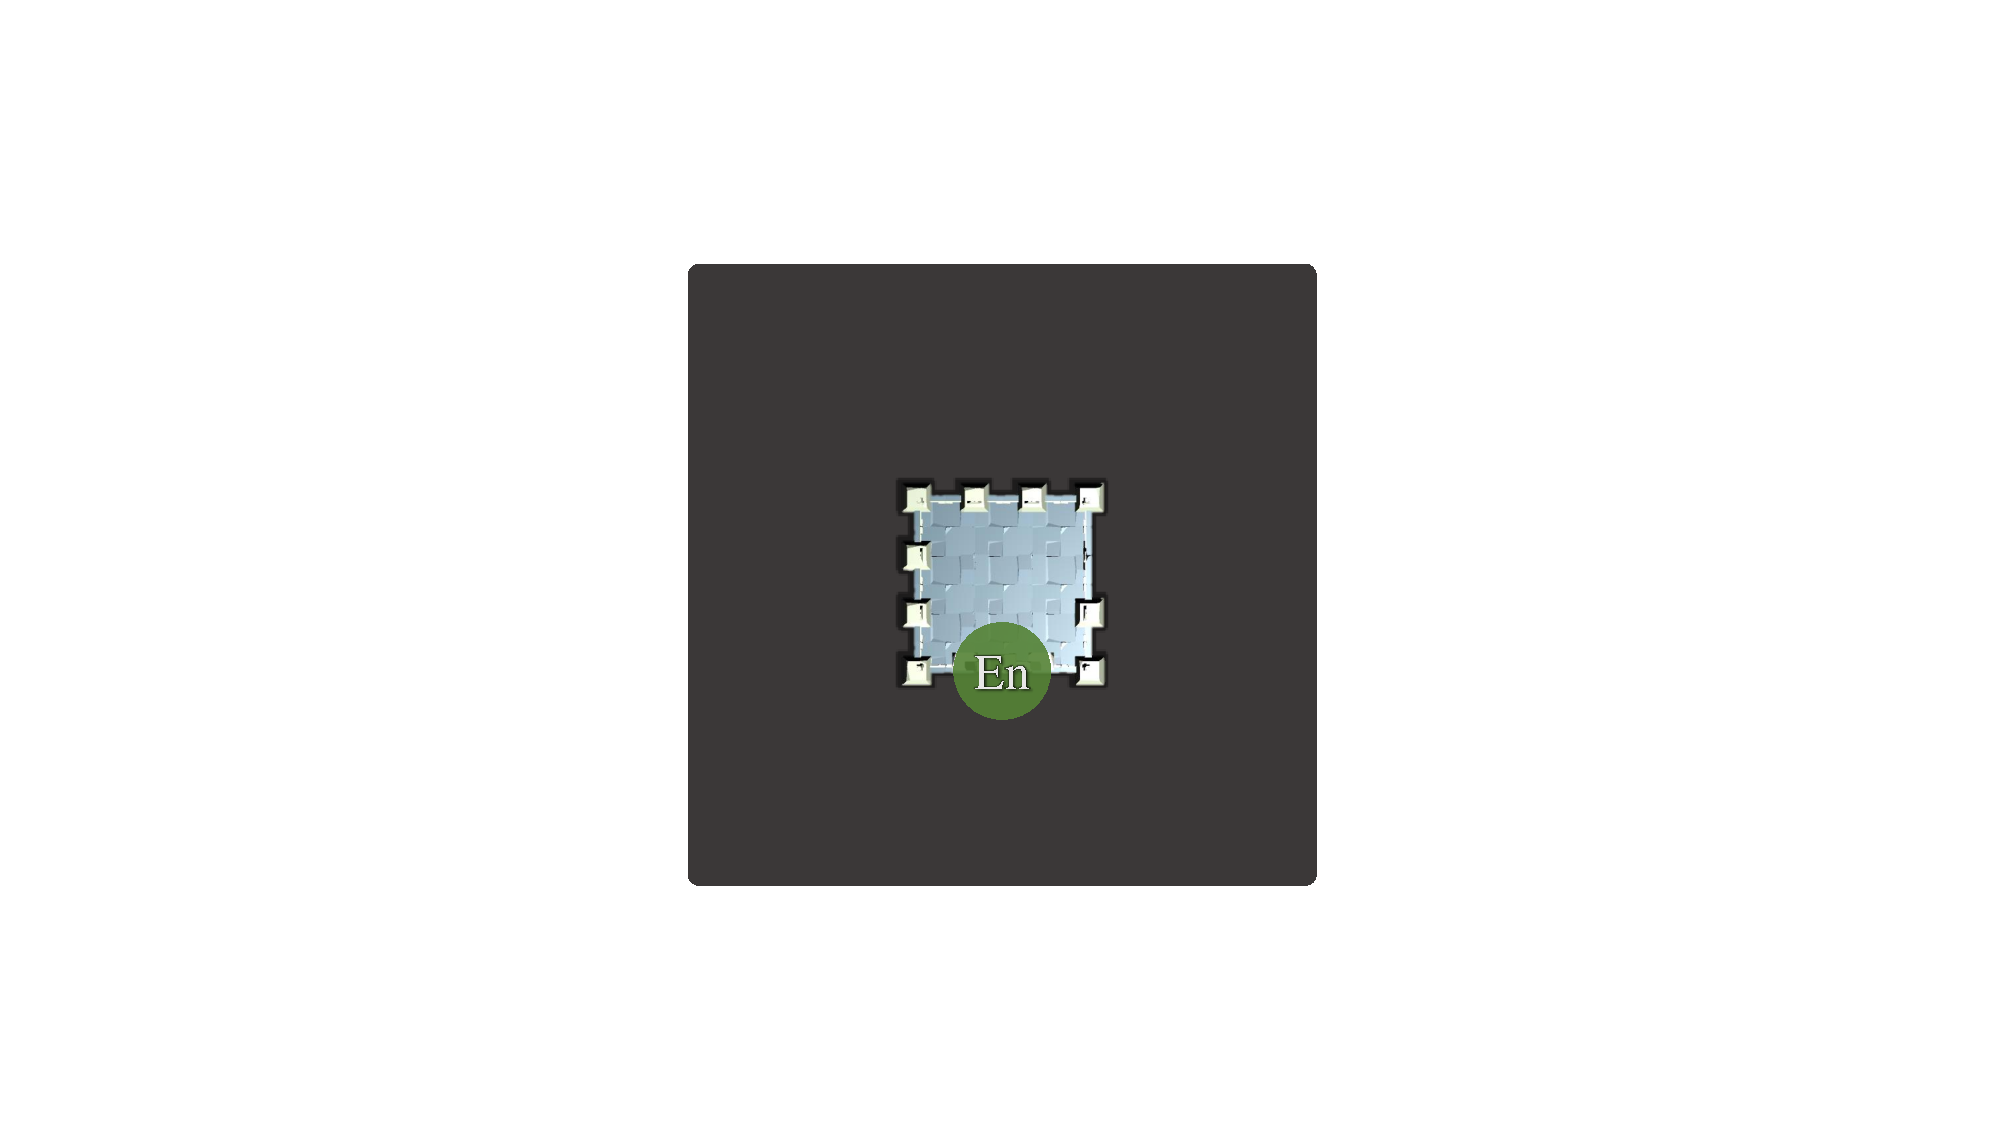
\includegraphics[width=1.0\textwidth]{figures/roomtype-wall.pdf}
    \caption{死路的房間容器結構}
    \label{fig:roomtype-wall}
  \end{center}
\end{figure}

\subsection{從任務圖轉為遊戲空間}
\label{ssec:method-spacepieces-frommissiontospace}

Joris Dormans 提到任務圖與空間圖應當是非常近似,甚至是二者同構~\cite{dormans2010adventures}。本小節將解釋 \textit{Dungeon Generator} 工具運行「將任務轉為空間的改寫系統」的流程,以及如何搭配任務圖的語法分析器。其一,藉由「建造方式表」(表~\ref{tbl:mission-to-space-instruction})將任務圖轉換成有意義拓撲關係的遊戲空間;其二,利用「空間替換表」(表~\ref{tbl:mission-to-space-replace})把前述遊戲空間不足之處補足。完成上述改寫系統進程後,便能夠輸出帶有任務邏輯的遊戲空間。演算法~\ref{alg:algorithm-mission-to-space-rewritesystem} 中,系統會遵循第~\ref{ssec:method-missiongrammars-graph} 小節產生的任務圖,以深度優先搜尋法遍歷任務圖,經過的源節點便從建造方式表中挑選出一個房間容器,逐一將各個終端節點轉換為實際空間,接著透過空間替換表,將場面上剩餘的端點識別物依序替換成對應房間容器,以完成遊戲空間之建置,相關演示可參考第~\ref{sssec:method-spacepieces-frommissiontospace-instruction}、~\ref{sssec:method-spacepieces-frommissiontospace-replacement} 二小節,將會逐一介紹演算法~\ref{alg:algorithm-mission-to-space-rewritesystem} 的實際應用流程。

\begin{algorithm}[!htb]
    \caption{改寫系統(任務轉換空間)}
    \label{alg:algorithm-mission-to-space-rewritesystem}
    \begin{algorithmic}[1]
        \Require
            \Statex $graph$ is $MissionGraph$.
            \Statex $seed$ is the random seed.
        \Ensure
            \State {Initialize random number generator via $seed$}                      \Comment{初始化亂數表,如 C 的 srand}
            \Statex
            \Function{RewriteSystem2}{$graph$}
                \ForAll {$node\in graph$}:                                              \Comment{Instrcution,第~\ref{sssec:method-spacepieces-frommissiontospace-instruction} 小節}
                    \State {$volume$ = GetVolumeFromInstructionTable($node$)}
                    \Statex                                                             \Comment{參照表~\ref{tbl:mission-to-space-instruction},受 Line $1$ 影響}
                    \State {$isSucceed$ = SetVolumeToSpace($volume$)}                   \Comment{圖~\ref{fig:mission-to-space-instruction-flow},受 Line $1$ 影響}
                    \If {$isSucceed$ is $false$}
                        \Return {$false$}
                    \EndIf
                \EndFor
                \ForAll {$marker\in ConnectionsInGraph$}:                               \Comment{Replacement,第~\ref{sssec:method-spacepieces-frommissiontospace-replacement} 小節}
                    \State {$volume$ = GetVolumeFromReplacementTable($marker$)}
                    \Statex                                                             \Comment{參照表~\ref{tbl:mission-to-space-replace},受 Line $1$ 影響}
                    \State {$isSucceed$ = SetVolumeToSpace($volume$)}                   \Comment{圖~\ref{fig:mission-to-space-replacement-result},受 Line $1$ 影響}
                    \If {$isSucceed$ is $false$}
                        \Return {$false$}
                    \EndIf
                \EndFor
                \State {\Return {$true$}}                                               \Comment{成功轉換成遊戲空間}
            \EndFunction
    \end{algorithmic}
\end{algorithm}

\subsubsection{建造方式}
\label{sssec:method-spacepieces-frommissiontospace-instruction}

為從已生成完畢的任務圖進而衍生出遊戲空間,在創建的房間容器會對應一任務符號表當中的終端符 (terminal symbols),稱作為建造方式 (building instruction)。本小節會利用第~\ref{ssec:method-missiongrammars-alphabet} 小節的任務符號表,過濾出終端節點並逐一對應至第~\ref{ssec:method-spacepieces-types} 小節的房間容器,見表~\ref{tbl:mission-to-space-instruction}。每一個終端節點都必須對應一個以上的房間容器,房間容器不允許被重複使用在不同的終端節點上。

\setlength\LTcapwidth{\linewidth}
\begin{longtable}{
    | >{\centering\arraybackslash} m{1.0cm}
    | >{\centering\arraybackslash} m{3.5cm}
    | >{} m{1.0cm}
    | >{\centering\arraybackslash} m{1.0cm}
    | >{\centering\arraybackslash} m{3.5cm} | }
  \caption{建造方式表,任務終端節點與房間容器對應之範例}\label{tbl:mission-to-space-instruction} \\
  \cline{1-2}\cline{4-5}
  節點 & 對應之房間容器 &  & 節點 & 對應之房間容器 \\
  \cline{1-2}\cline{4-5}
  \endfirsthead
  \multicolumn{5}{c}%
  {\tablename\ \thetable\ -- \textit{接續前頁面}} \\
  \cline{1-2}\cline{4-5}
  節點 & 對應之房間容器 &  & 節點 & 對應之房間容器 \\
  \cline{1-2}\cline{4-5}
  \endhead
  \multicolumn{5}{r}{\textit{接續下頁面}} \\
  \endfoot
  \endlastfoot
  \missionalphabetnode{t-entrance}{10mm}
    & \missioninstruction{instruction-01}
    &
    & \missionalphabetnode{t-goal}{10mm}
    & \missioninstruction{instruction-02}
    \\\cline{1-2}\cline{4-5}
  \missionalphabetnode{t-boss}{10mm}
    & \missioninstruction{instruction-03}
    &
    & \missionalphabetnode{t-normal}{10mm}
    & \missioninstruction{instruction-04}
    \\\cline{1-2}\cline{4-5}
  \missionalphabetnode{t-normal}{10mm}
    & \missioninstruction{instruction-05}
    &
    & \missionalphabetnode{t-normal}{10mm}
    & \missioninstruction{instruction-06}
    \\\cline{1-2}\cline{4-5}
  \missionalphabetnode{t-normal}{10mm}
    & \missioninstruction{instruction-07}
    &
    & \missionalphabetnode{t-bomb}{10mm}
    & \missioninstruction{instruction-08}
    \\\cline{1-2}\cline{4-5}
  \missionalphabetnode{t-secret}{10mm}
    & \missioninstruction{instruction-09}
    &
    & \missionalphabetnode{t-lock}{10mm}
    & \missioninstruction{instruction-10}
    \\\cline{1-2}\cline{4-5}
  \missionalphabetnode{t-shop}{10mm}
    & \missioninstruction{instruction-11}
    &
    & \missionalphabetnode{t-treasure}{10mm}
    & \missioninstruction{instruction-12}
    \\\cline{1-2}\cline{4-5}
\end{longtable}

圖~\ref{fig:mission-to-space-instruction-flow} a 為使用第~\ref{ssec:method-missiongrammars-rules} 小節的任務規則表(表~\ref{tbl:missiongrammars-rules-linear-example}-~\ref{tbl:missiongrammars-rules-nonlinear-example3})所生成的任務圖,該階段採用的亂數種子為 $0$。本階段中,依照演算法~\ref{alg:algorithm-mission-to-space-rewritesystem} - 改寫系統(任務轉換空間),並且結合表~\ref{tbl:mission-to-space-instruction} 的建造方式表,將任務圖轉換為遊戲空間。圖~\ref{fig:mission-to-space-instruction-flow} 中,第一個節點起點 (entrance\missionalphabetnode{t-entrance}{5mm}) 直接對應到「起點房間容器」,而起點房間容器中擁有三個出口端點,系統將會亂數隨機一個出口端點進行後續房間生成,根據深度優先搜尋法下一個遍歷的節點為第二行的一般房 (normal\missionalphabetnode{t-normal}{5mm}),接著從建造方式表中過濾出能夠使用的四種「通道房間容器」,由系統亂數決定本次採用的房間容器後,將預計新增的房間容器之起點與前一步驟決定的出口端點進行房間容器連接,下一回合將從新增的房間容器重複前述之步驟。依照上述之步驟,改寫系統(任務轉換空間)完整遍歷所有的任務節點後,便能夠完成任務轉換空間的動作,結果可參考圖~\ref{fig:mission-to-space-instruction-result}。

進行疊代的過程時,以下幾種情形,疊代生成將會失敗:當任務圖節點的子節點數量大於對應房間容器的出口數量;當新生長的房間容器於其它房間容器發生碰撞。因此,若有以上違例情況,關卡設計師必須修正其關卡設計,如調整房間容器之格局或更換一筆亂數種子,並重新執行前述步驟。

\begin{figure}[!htb]
  \begin{center}
    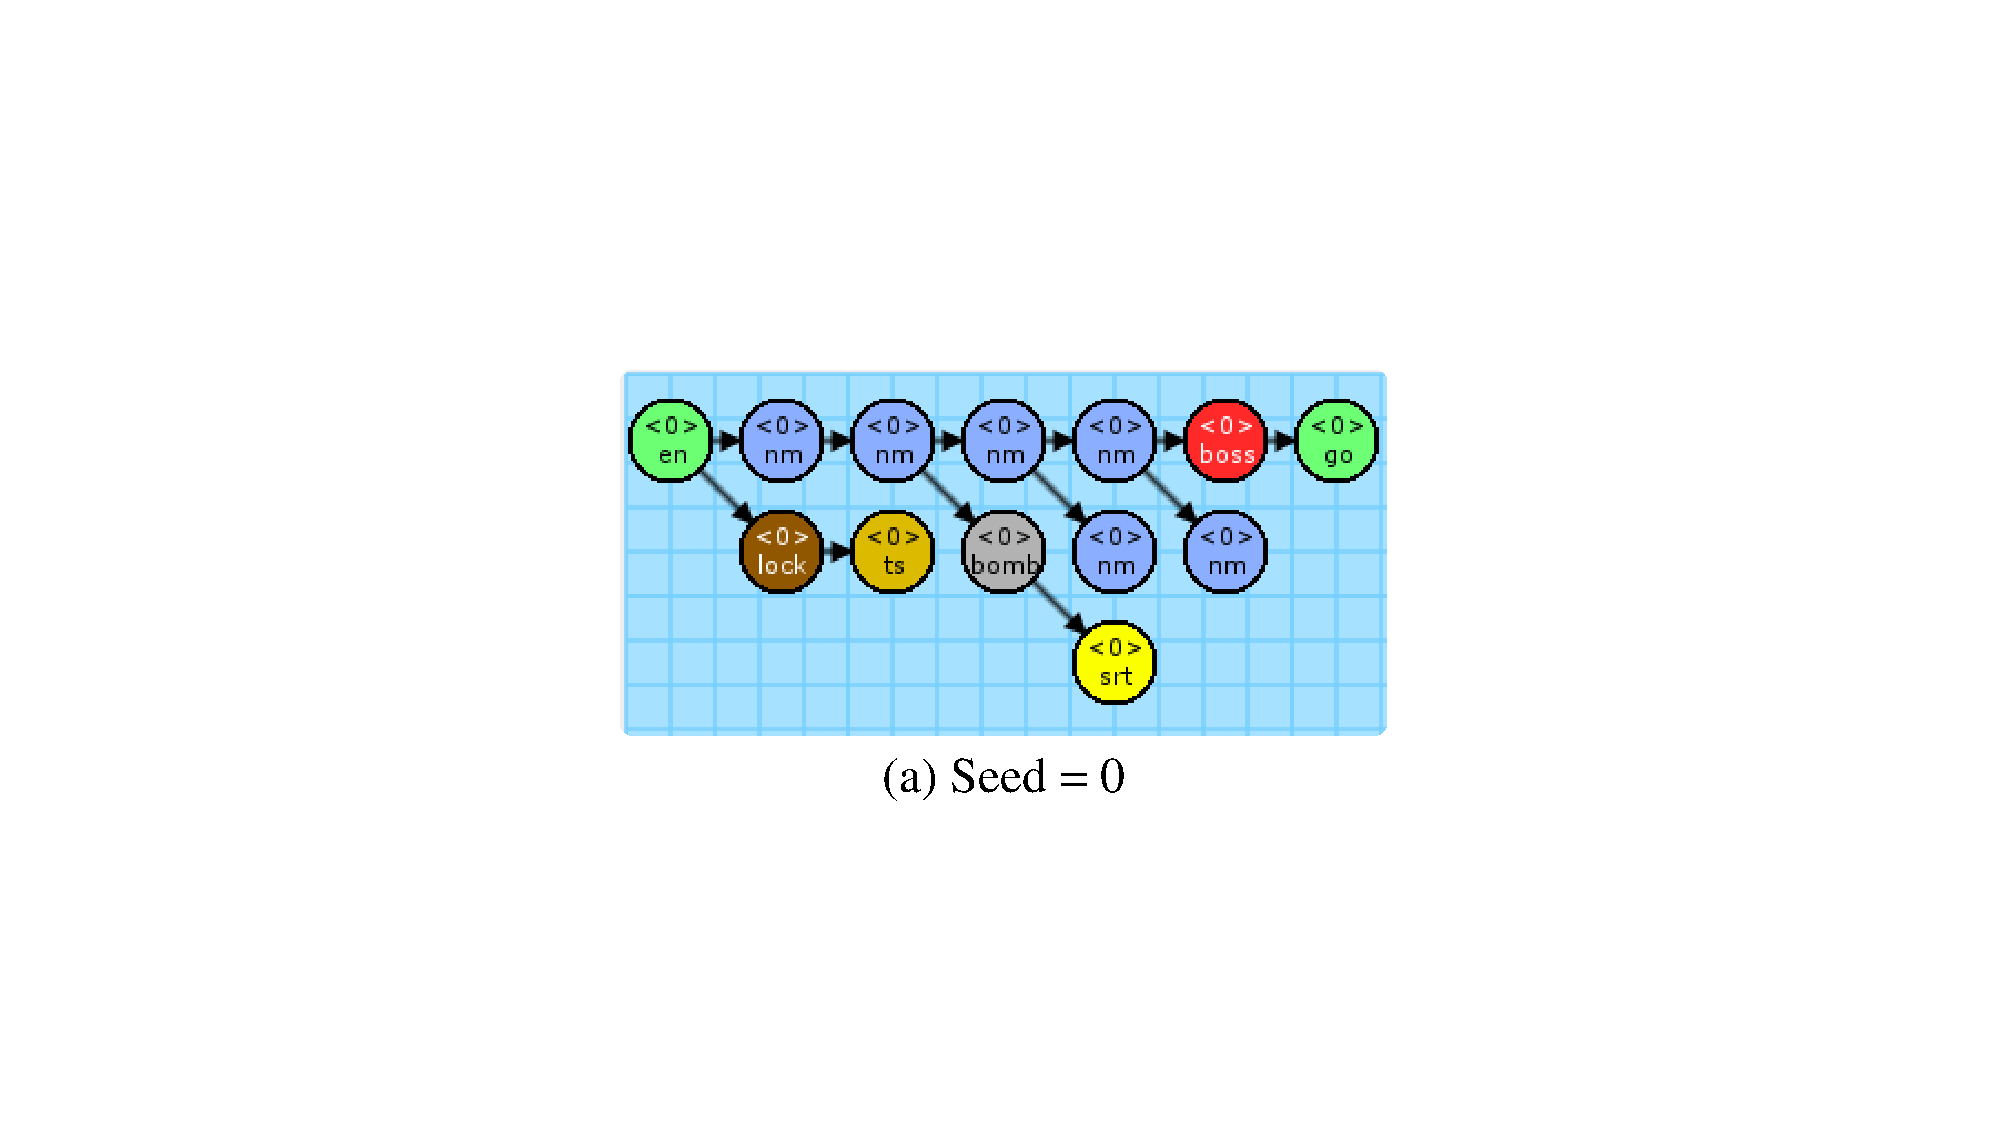
\includegraphics[width=1.0\textwidth]{figures/mission-to-space-instruction-flow.pdf}
    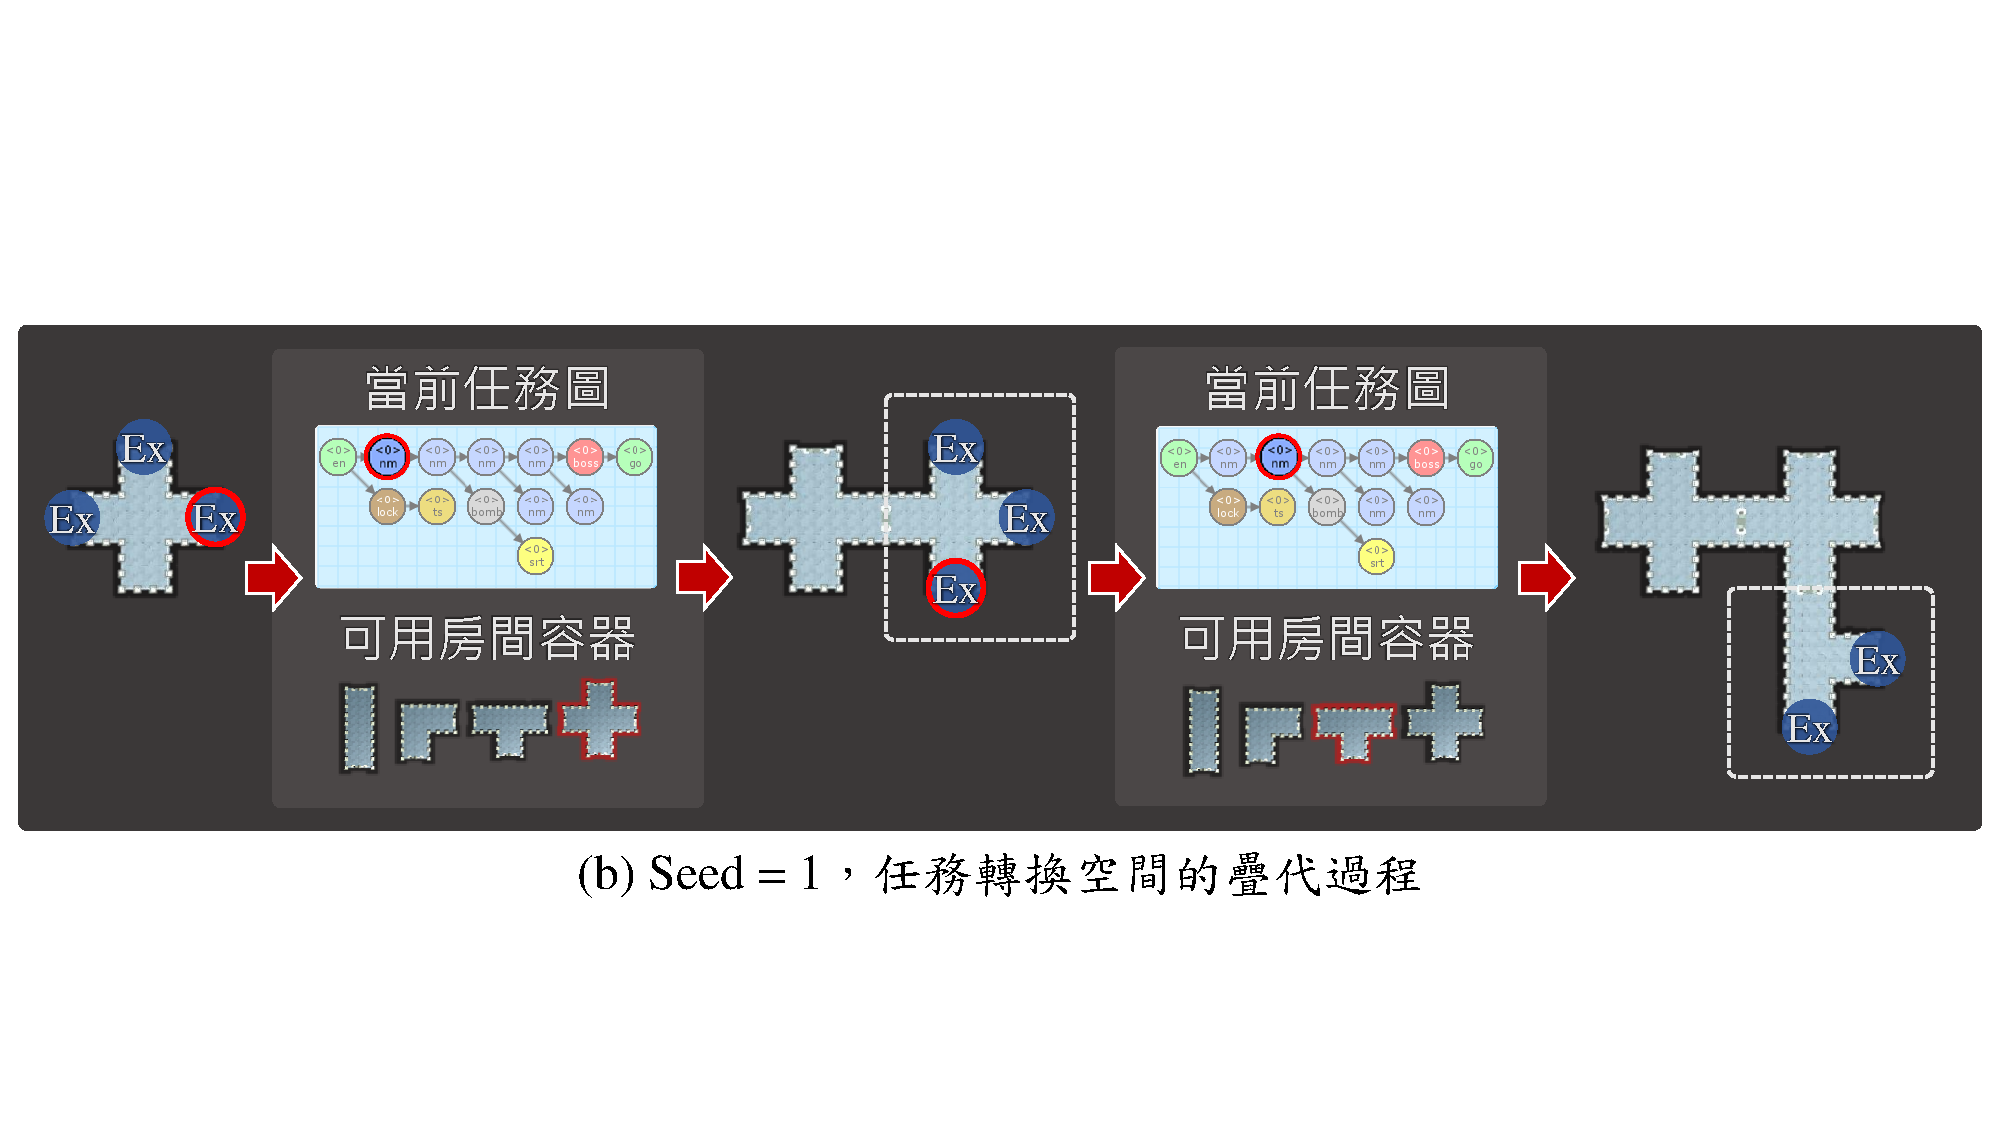
\includegraphics[width=1.0\textwidth]{figures/mission-to-space-instruction-flow-.pdf}
    \caption{建造方式的疊代生成過程} 
    \label{fig:mission-to-space-instruction-flow}
  \end{center}
\end{figure}

基於建造方法的對應紀錄,給予一亂數種子能夠確保能夠對應到一固定空間。當終端節點對應到複數房間容器時,亂數種子將影響從多個房間容器之間的順序。若生成過程中,該房間容器擁有多個出口,亦是參照亂數種子決定調用出口生成之順序,見圖~\ref{fig:mission-to-space-instruction-result}。

\begin{figure}[!htb]
  \begin{center}
    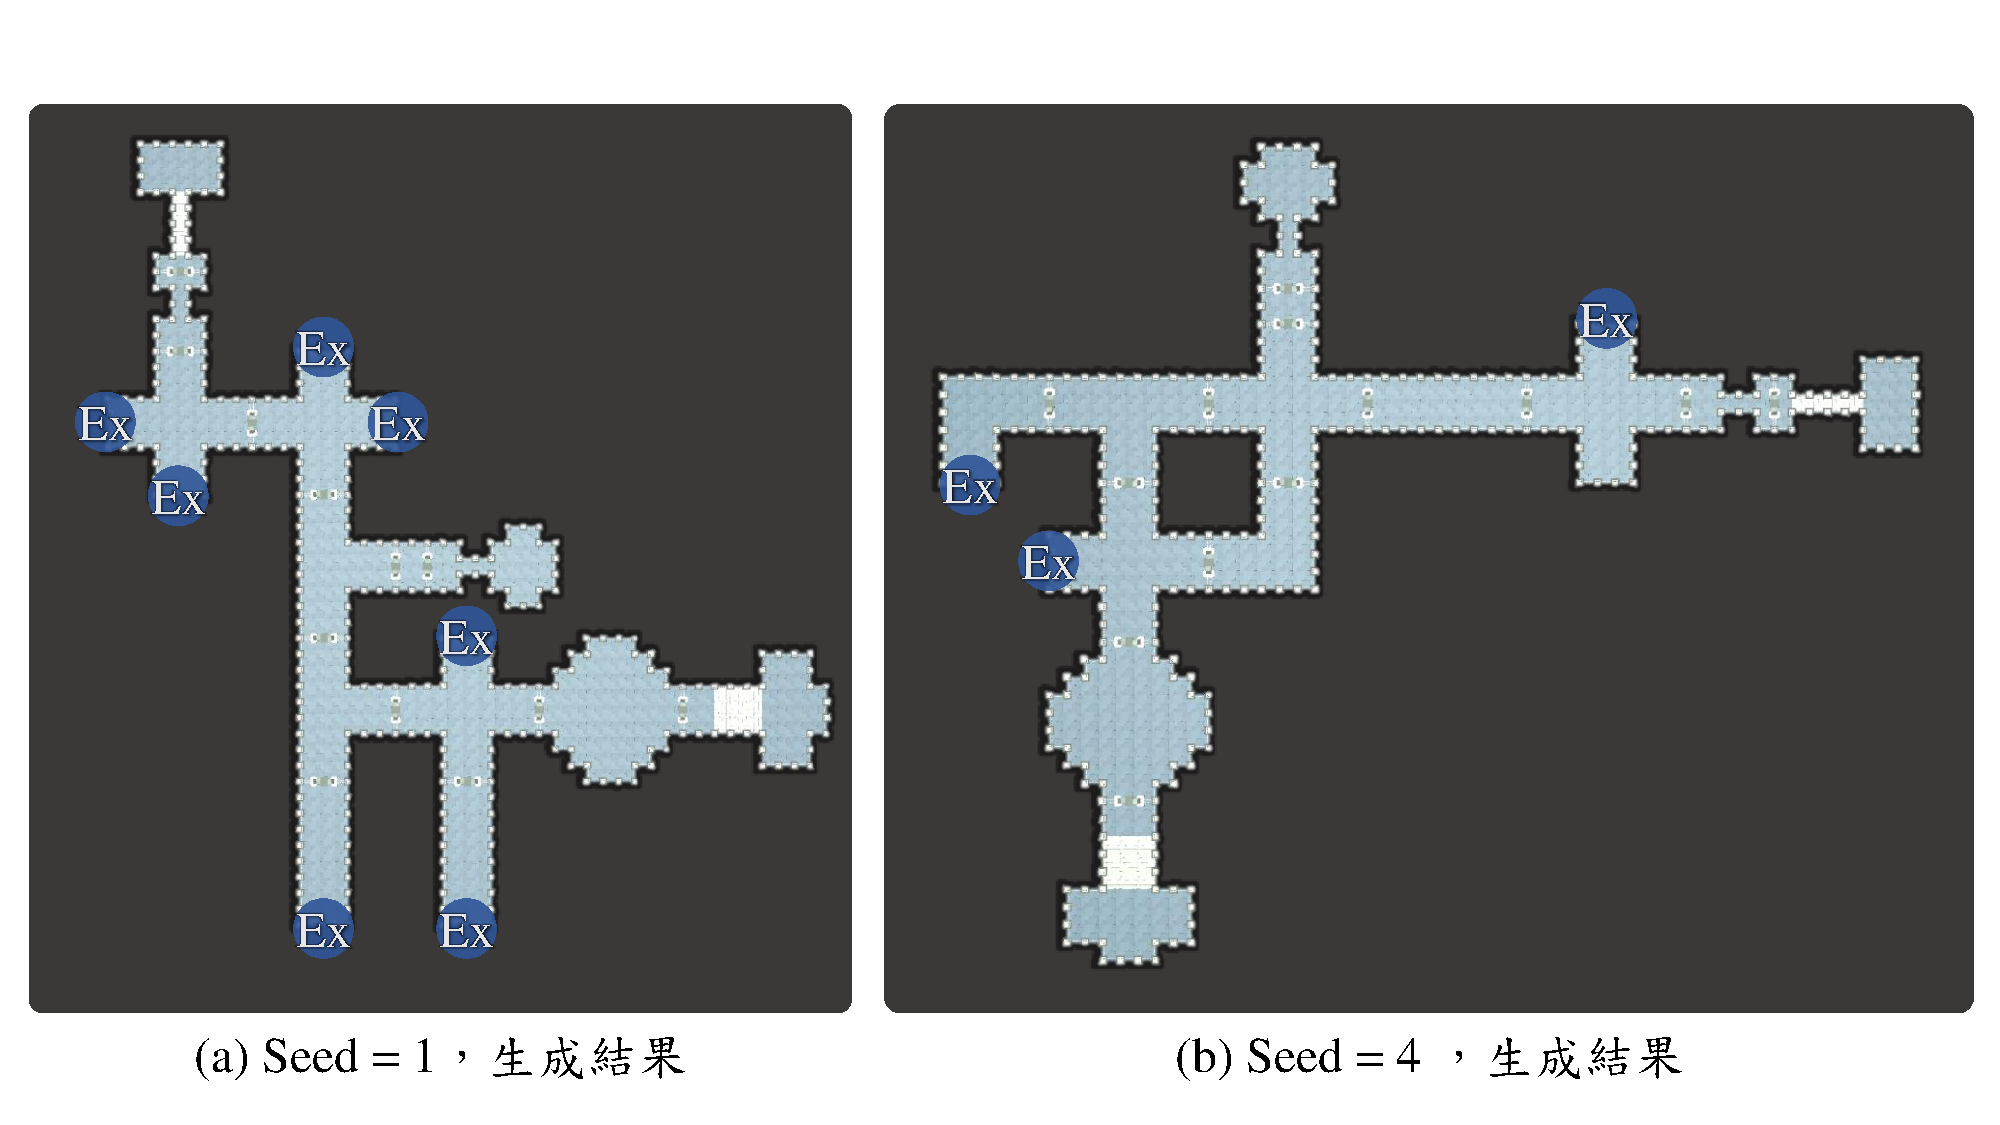
\includegraphics[width=1.0\textwidth]{figures/mission-to-space-instruction-result.pdf}
    \caption{已疊代生成的任務圖,不同亂數種子轉換為對應結果的遊戲空間} 
    \label{fig:mission-to-space-instruction-result}
  \end{center}
\end{figure}

\subsubsection{剩餘空間替換}
\label{sssec:method-spacepieces-frommissiontospace-replacement}

一個端點識別物能夠對應複數個房間容器,房間容器能夠重複被不同的端點識別物所對應。第~\ref{ssec:method-spacepieces-connections} 小節,介紹端點識別物時,曾提及到遊戲設計師能夠自由擴充出口識別物的種類。

在此為簡化範例,表~\ref{tbl:mission-to-space-replace} 採用預設之單一出口識別物,而這項出口識別物將對應圖~\ref{fig:roomtype-wall} 的死路房間容器,左側為端點識別物之種類,右側為所對應的房間容器。

\begin{table}[!htb]
  \centering
  \caption{空間替換表,出口端點與房間容器對應之範例}
  \label{tbl:mission-to-space-replace}
  \bigskip
  \vspace{-5mm}
  \begin{tabular}{
    | >{\centering\arraybackslash} m{1.5cm}
    | >{\centering\arraybackslash} m{3.5cm} | }
    \hline
    \multicolumn{1}{ |c| }{端點}
      & \multicolumn{1}{ c| }{對應之房間容器} \\\hline
    \begin{minipage}{.3\textwidth}
\includegraphics[width=15mm]{figures/mission-grammars-ins-rep/replacement-l-01.png}\end{minipage}
      & \begin{minipage}{.3\textwidth}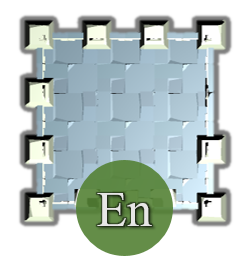
\includegraphics[width=35mm]{figures/mission-grammars-ins-rep/replacement-r-01.png}\end{minipage}
      \\\hline
  \end{tabular}
\end{table}

在圖~\ref{fig:mission-to-space-instruction-result} 可觀察到,經過建造方式的遊戲空間仍會遺留部分的端點識別物,為了將其延伸或予以封閉,本小節將進行替換 (replacement) 使遊戲空間趨於完整,見圖~\ref{fig:mission-to-space-replacement-result}。若增加空間替換表其對應的選項,便能創造出主線外的分支結構。

\begin{figure}[!htb]
  \begin{center}
    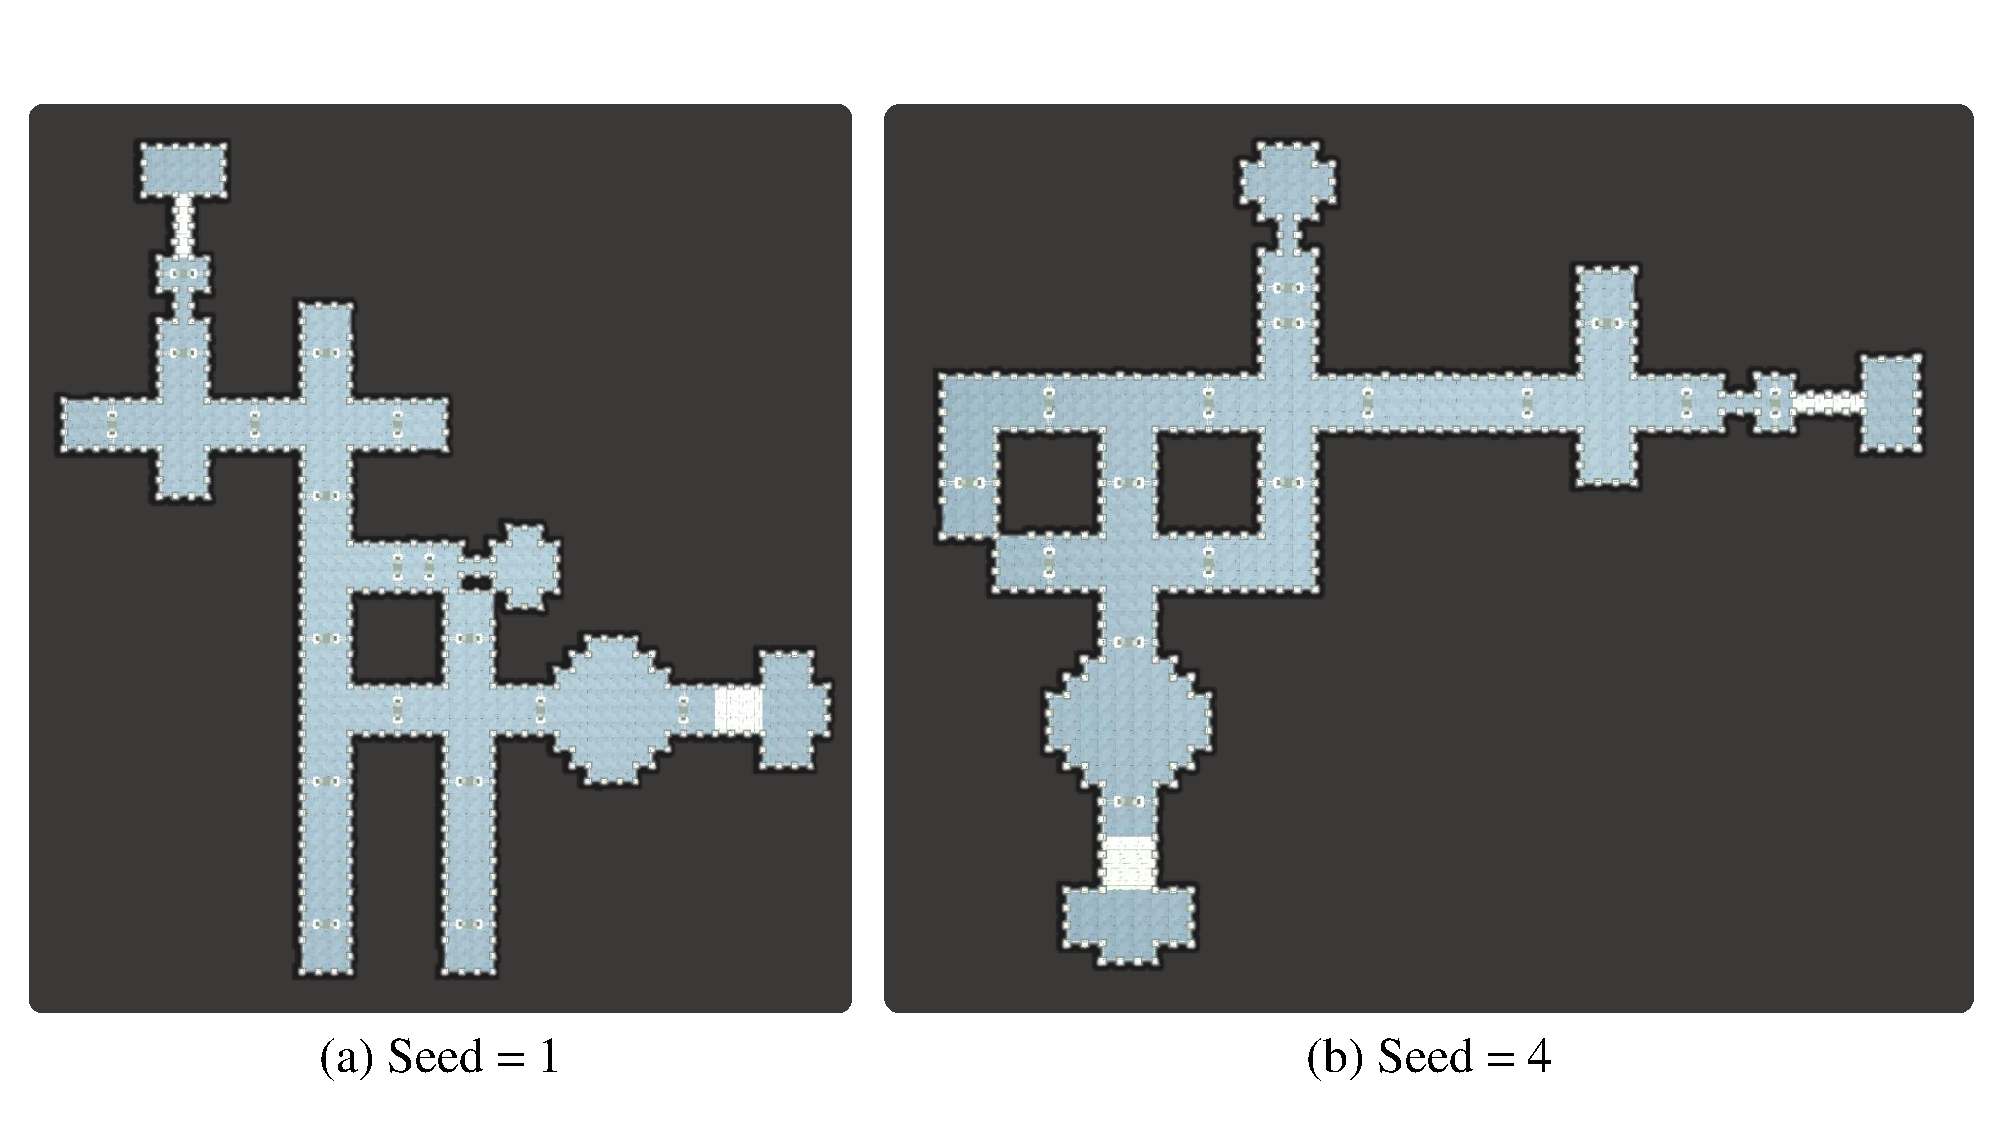
\includegraphics[width=1.0\textwidth]{figures/mission-to-space-replacement-result.pdf}
    \caption{經過剩餘空間替換後的完整遊戲空間} 
    \label{fig:mission-to-space-replacement-result}
  \end{center}
\end{figure}

% Clean the page after this section.
\clearpage

\section{地圖片段}
\label{sec:method-segments}

為了將第~\ref{ssec:relatedworks-proceduralgamepatterns} 小節提及的程序化遊戲物件擺放技術付諸實現,構築出遊戲內部的複雜系統,讓玩家體驗到突現型 (emergence) 的遊玩機制,我們將延續上一節的遊戲關卡結構,參考 Antonios Liapis 提出的地圖片段演化方法~\cite{liapis2017multi},令地圖片段為房間容器,並進行改良以合適我方實驗環境。

圖~\ref{fig:segments-with-ga} 介紹地圖片段的演化流程。第一步驟,基於第~\ref{ssec:method-segments-gene} 小節中定義的基因結構,產生初始父母代族群時,讓全部的基因先預設為空磚;第二步驟,透過適應性函數計算各個體的適應值 (fitnesses),完整的適應性函數在第~\ref{ssec:method-segments-fitnesses} 小節中說明;第三步驟將會從族群中挑選最優異的兩個父母染色體,高機率進行交配,若無進行交配將會將子代沿用父母代的基因;第四步驟有低機率讓衍生的子代進行突變;第五步驟以新的衍生子代取代舊有的父母代族群;第六步驟會檢查是否達到終止條件,若尚未滿足終止條件,便會回到第二步驟,直到輸出最適解。前述之交配、突變事件的機率與其方法屬於實驗變因,將在第~\ref{cha:experiment} 章進行定義與相關釋義。

\begin{figure}[!htb]
  \begin{center}
    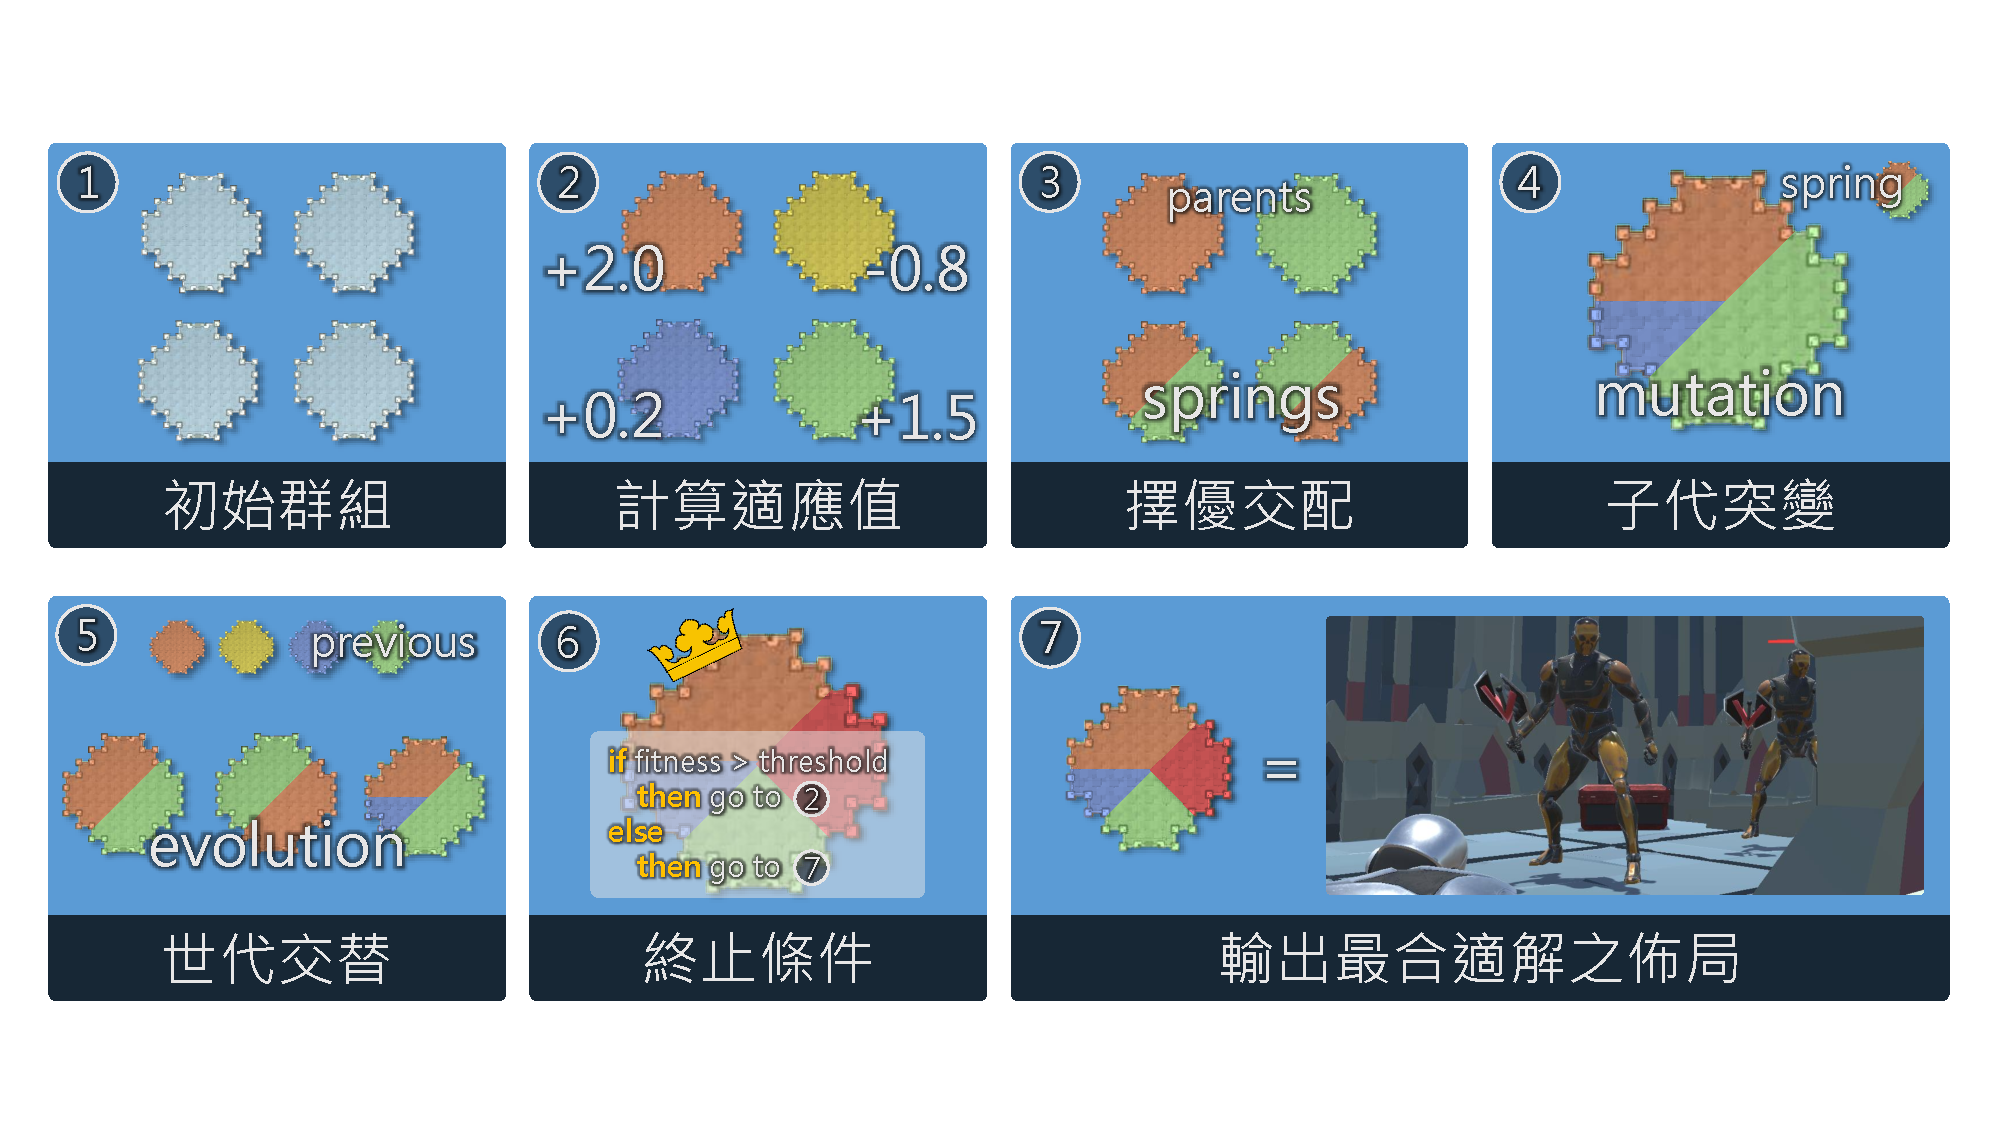
\includegraphics[width=1.0\textwidth]{figures/segments-with-ga.pdf}
    \caption{房間容器採取基因演算法之演化流程} 
    \label{fig:segments-with-ga}
  \end{center}
\end{figure}

\subsection{基因的儲存結構}
\label{ssec:method-segments-gene}

圖~\ref{fig:segments-gene-expression} a 是遊戲物件的表型 (phenotype),為基因演算法中的個體單位,房間容器能夠存放數種遊戲物件,分別為空磚 (Empty)、敵人磚 (Enemy)、寶箱磚 (Treasure) 與陷阱磚 (Trap),圖中帶有編號的位置意指著該座標能夠擺放遊戲物件,且玩家角色能夠在該座標通過;遊戲物件的擺放位置為個體的染色體 (chromosome),以一維陣列之基因序列表示,見圖~\ref{fig:segments-gene-expression} b;基因序列中的基因,會存放該座標的相對位置與遊戲物件類型,見圖~\ref{fig:segments-gene-expression} c。同一個房間容器會擁有許多不同的個體,這些個體的集合便是族群 (population)。

\begin{figure}[!htb]
  \begin{center}
    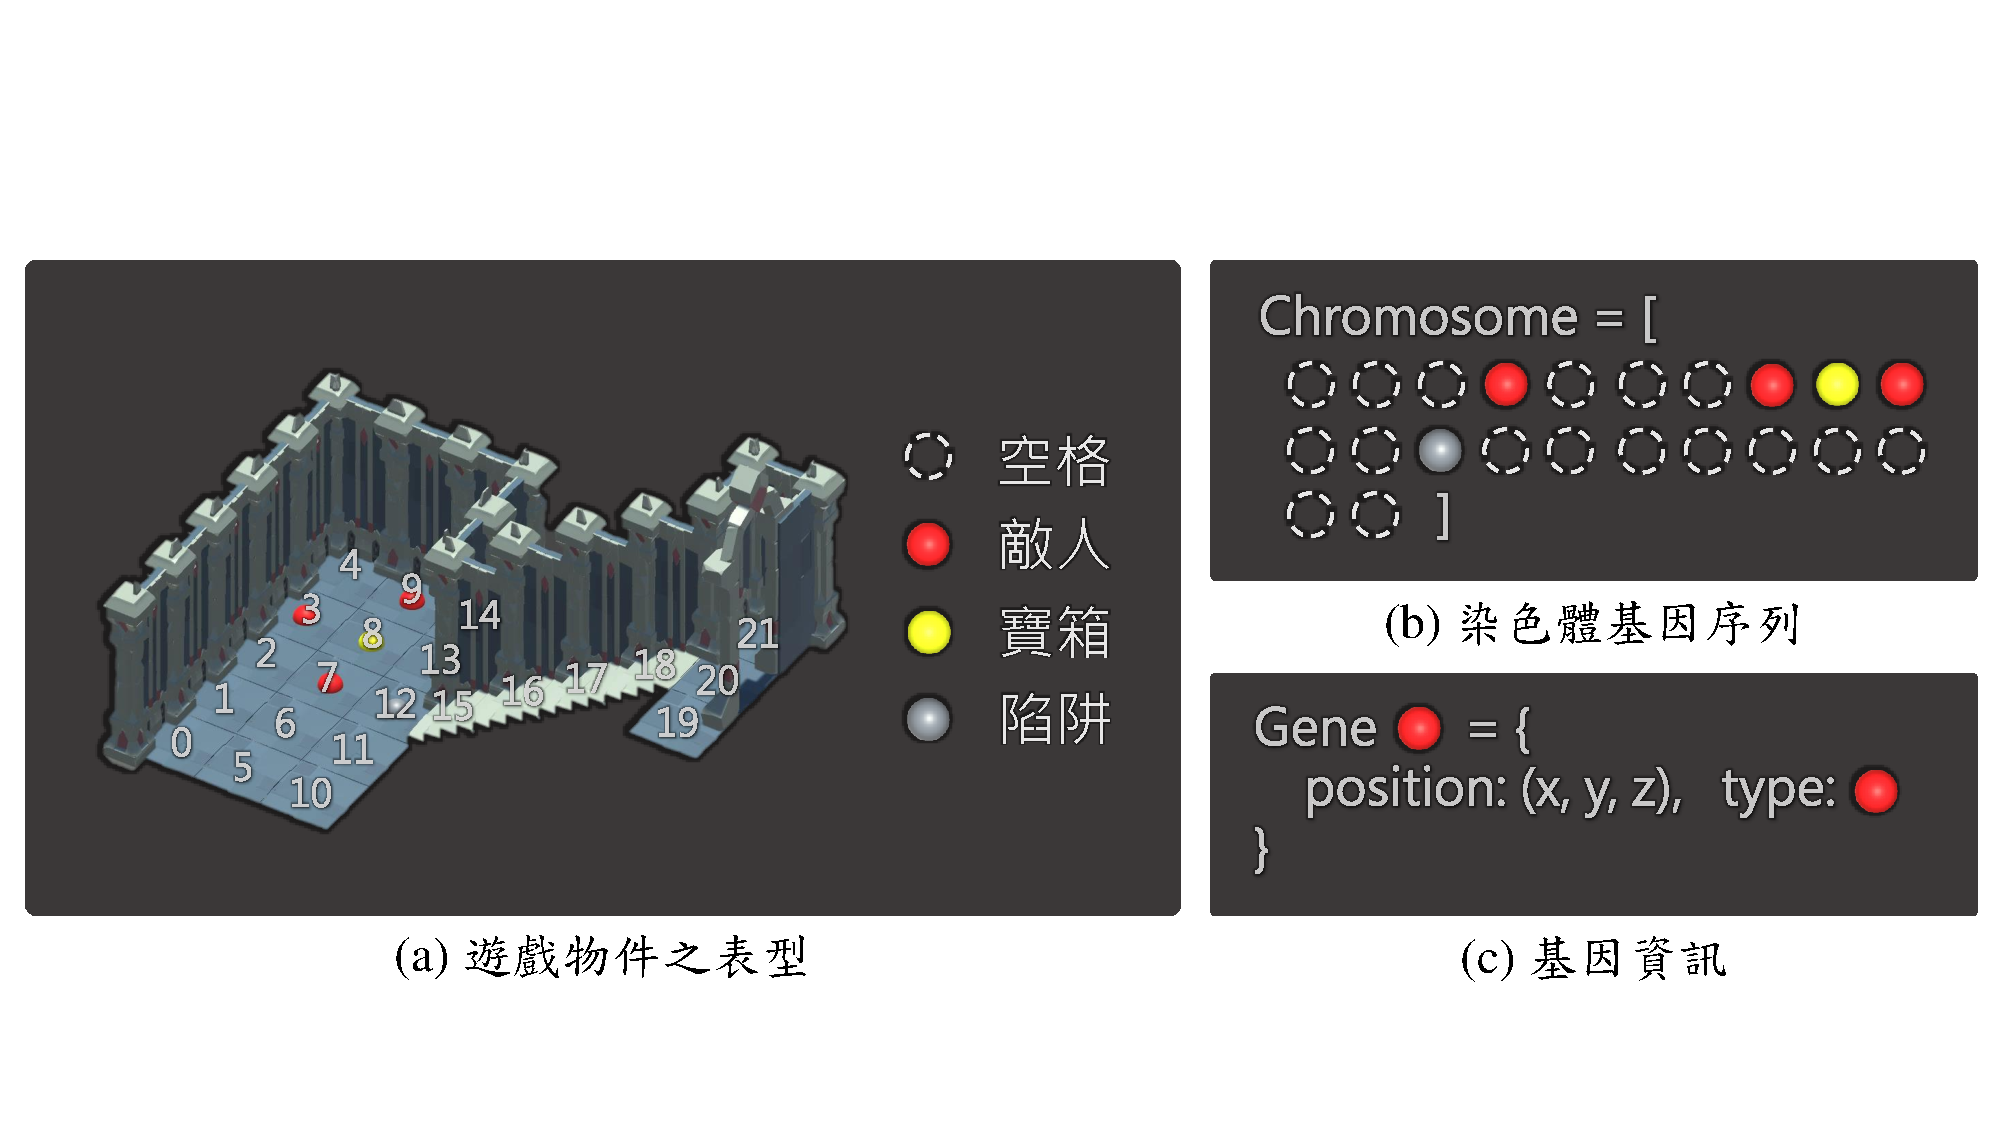
\includegraphics[width=1.0\textwidth]{figures/segments-gene-expression.pdf}
    \caption{房間容器以遊戲物件的佈局方式作為染色體}
    \label{fig:segments-gene-expression}
  \end{center}
\end{figure}

\subsection{演化之適應性函數}
\label{ssec:method-segments-fitnesses}

動作冒險遊戲 (A-AVG)、動作角色扮演遊戲 (A-RPG) 等類型遊戲,多可見一些制式化遊戲物件的搭配組合,Alexander Baldwin 認為遊戲物件組合的細觀特徵 (Meso-Patterns) 需要有檢測其品質的方法~\cite{baldwin2017mixed}。我們嘗試汲取出多項遊玩特徵並參數化公式,作為評估關卡品質的指標之一。

於前處理階段時,圖~\ref{fig:decorations-with-directions} 中顯示的地面、階梯裝飾物屬於可以通行的瓦磚單位(請參考圖~\ref{fig:decorations-with-directions} a-b)。圖~\ref{fig:fitnesses-mainpath} 使用 A-Star 搜尋演算法~\cite{hart1968formal} 建立行走空間,並搜索入口至多個出口的最短路徑,凡經過的座標稱作為空間動線 ($MP$) 之一,並將其權重值 ($mp$) 增加 $1$,空間動線為多項指標關鍵性的參考依據。倘若遇到無法計算最短路徑的情形,便不存在空間動線,屆時該房間容器將不能夠套用相關適應性函數。

\begin{figure}[!htb]
  \begin{center}
    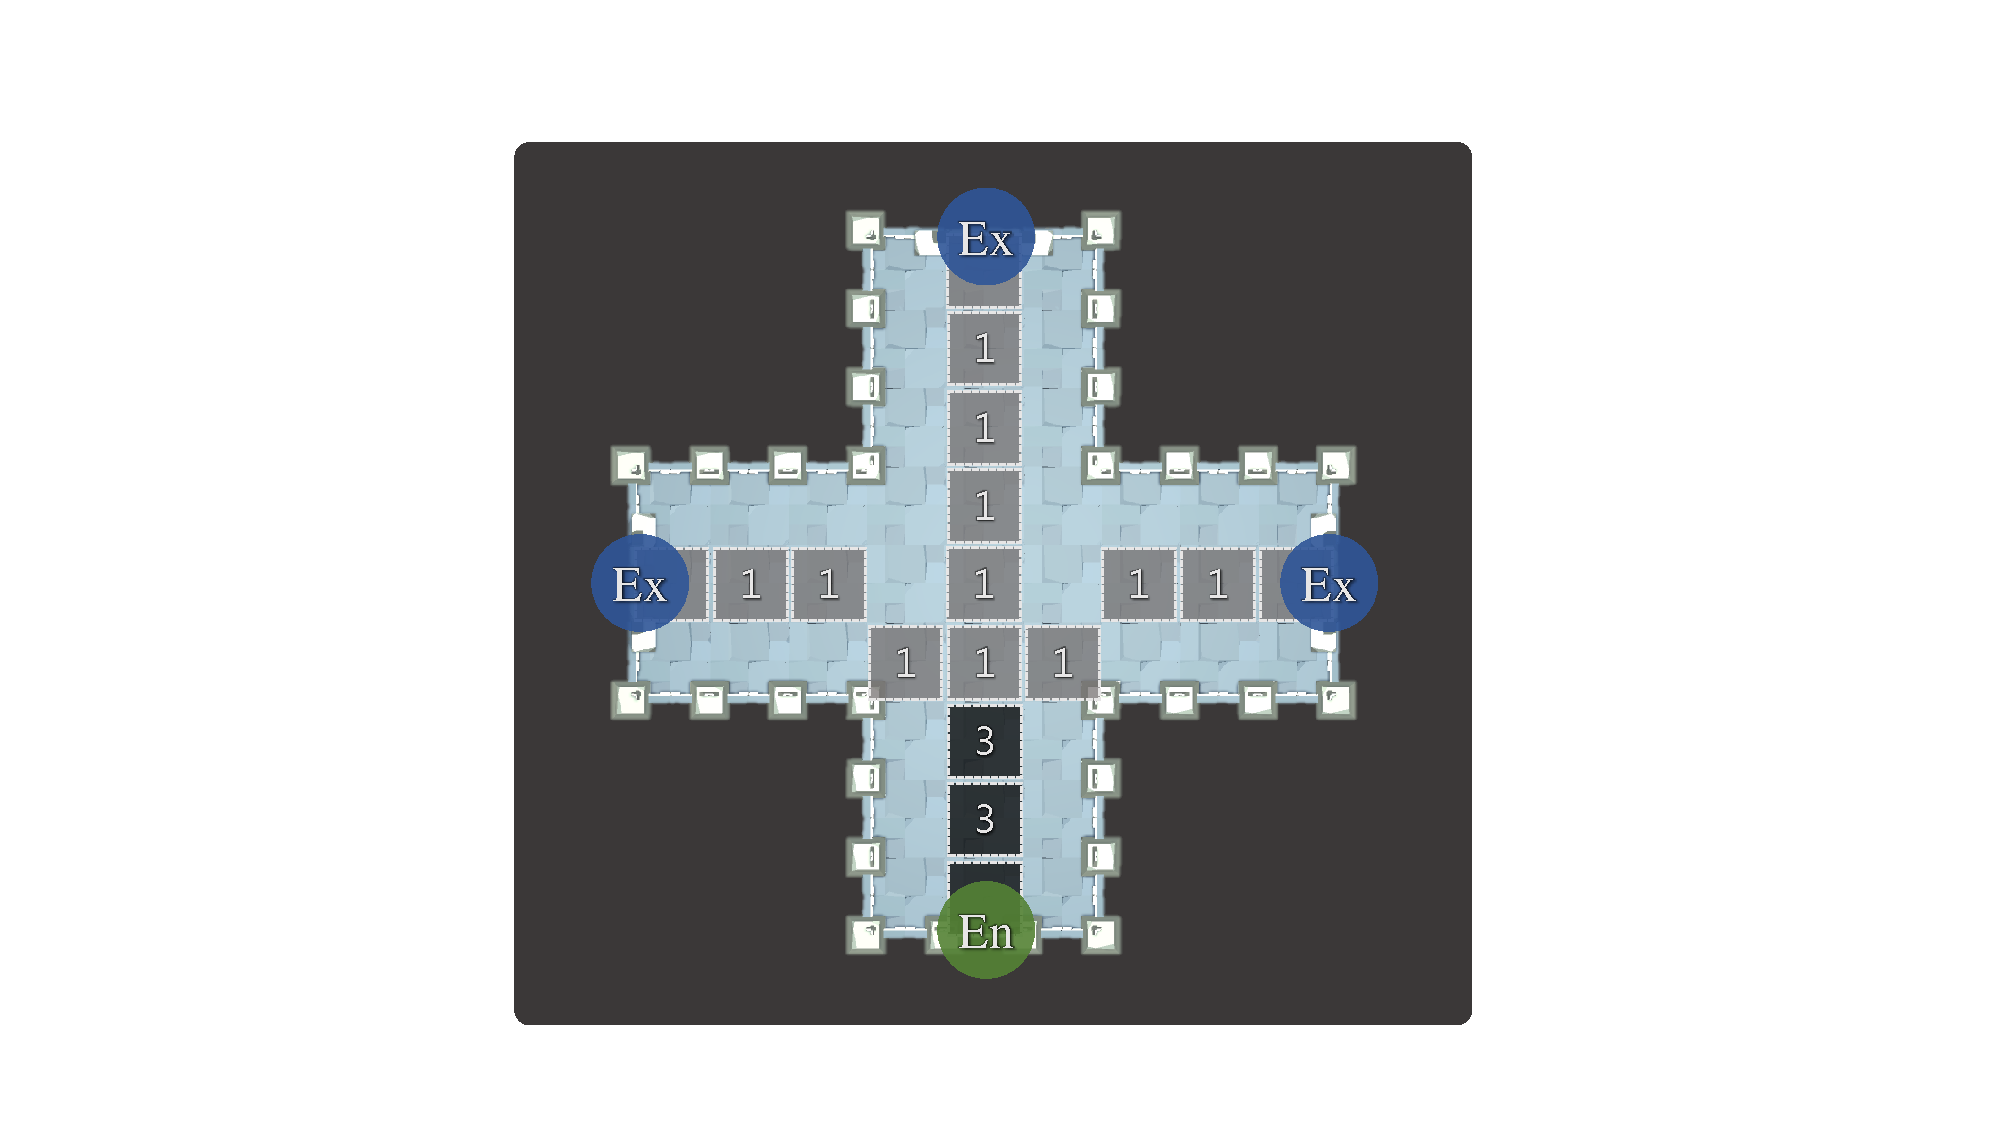
\includegraphics[width=1.0\textwidth]{figures/fitnesses-mainpath.pdf}
    \caption{動線於房間容器的計算方式,圖中數值為行經次數}
    \label{fig:fitnesses-mainpath}
  \end{center}
\end{figure}

\subsubsection{守衛點 (Guard)}
\label{sssec:method-segments-fitnesses-guard}

方程式~\ref{eq:fitnesses-guard} 為守衛點的適應性函數。為體現出敵人會保衛寶箱 ($Treasure$) 與出口 ($Exit$) 的現象,計算敵人 ($E_{i}$) 與為守護對象的遊戲物件 ($O_{j}$) 之間的距離,倘若距離愈近則帶來的影響力愈大。

\begin{equation}
    \label{eq:fitnesses-guard}
    f_{grd} = \sum_{i=1}^{M} \sum_{j=1}^{N} \frac{1}{dist\big(E_{i}, O_{j}\big)}, O_{j} \in \{ Treasure, Exit \}
\end{equation}

\begin{figure}[!htb]
  \begin{center}
    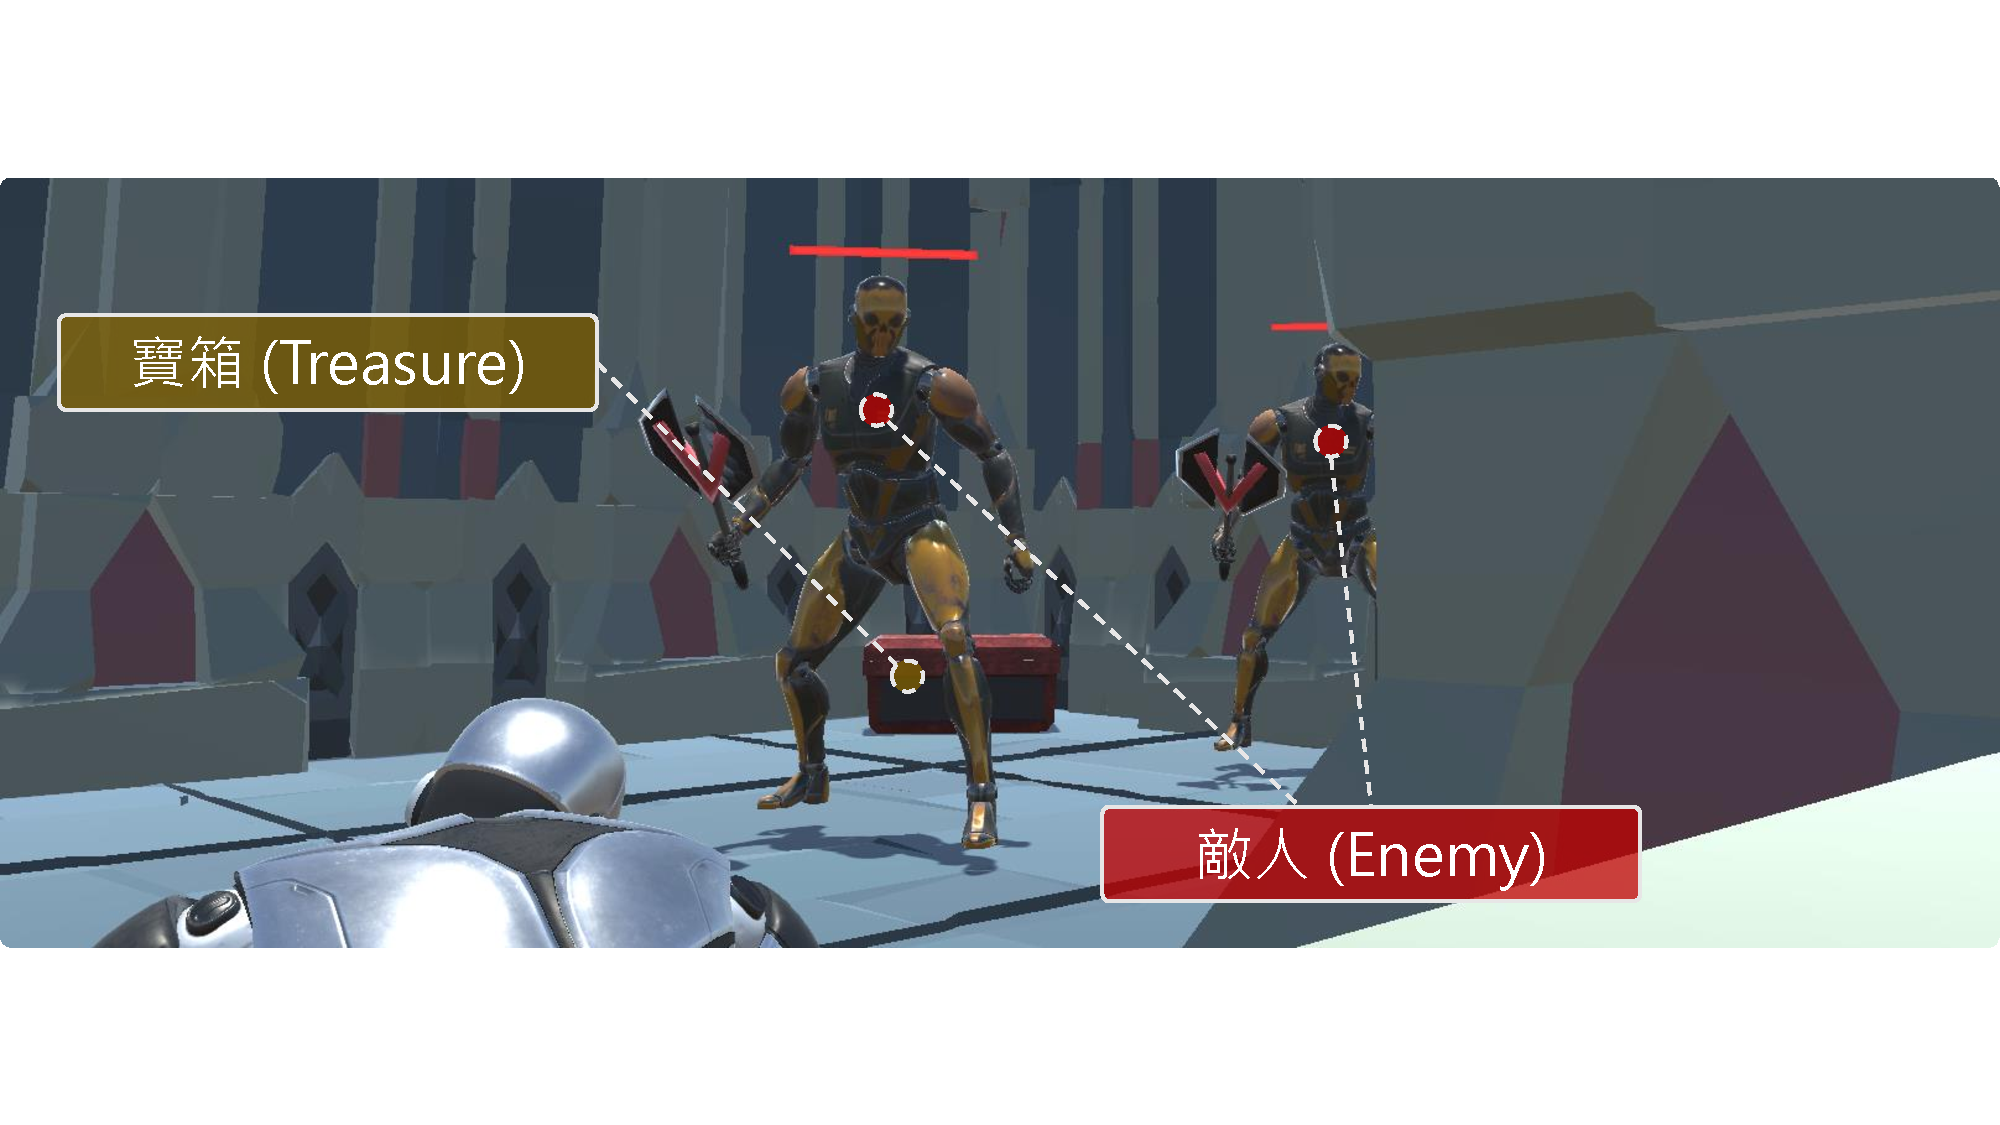
\includegraphics[width=1.0\textwidth]{figures/fitnesses-guard-gameplay.pdf}
    \caption{守衛點指標的遊戲體現情形}
    \label{fig:fitnesses-guard-gameplay}
  \end{center}
\end{figure}

\subsubsection{阻擋點 (Block)}
\label{sssec:method-segments-fitnesses-block}

方程式~\ref{eq:fitnesses-block} 為阻擋點的適應性函數。敵人會專注於阻擋玩家繼續前進,迫使玩家與其發生衝突。$f_{blk}$ 為加總 $M$ 個敵人於空間之動線權重 ($e_{i}$),倘若敵人並未落在動線上,權重則為 $0$。圖~\ref{fig:fitnesses-block-gameplay} 為阻擋點指標的實際遊玩情形,草綠色區塊為系統計算出的空間動線的瓦磚,敵人將會被設置於動線之上阻擋玩家前行。

\begin{equation}
    \label{eq:fitnesses-block}
    f_{blk} = \sum_{i=1}^{M} e_{i}
\end{equation}

\begin{figure}[!htb]
  \begin{center}
    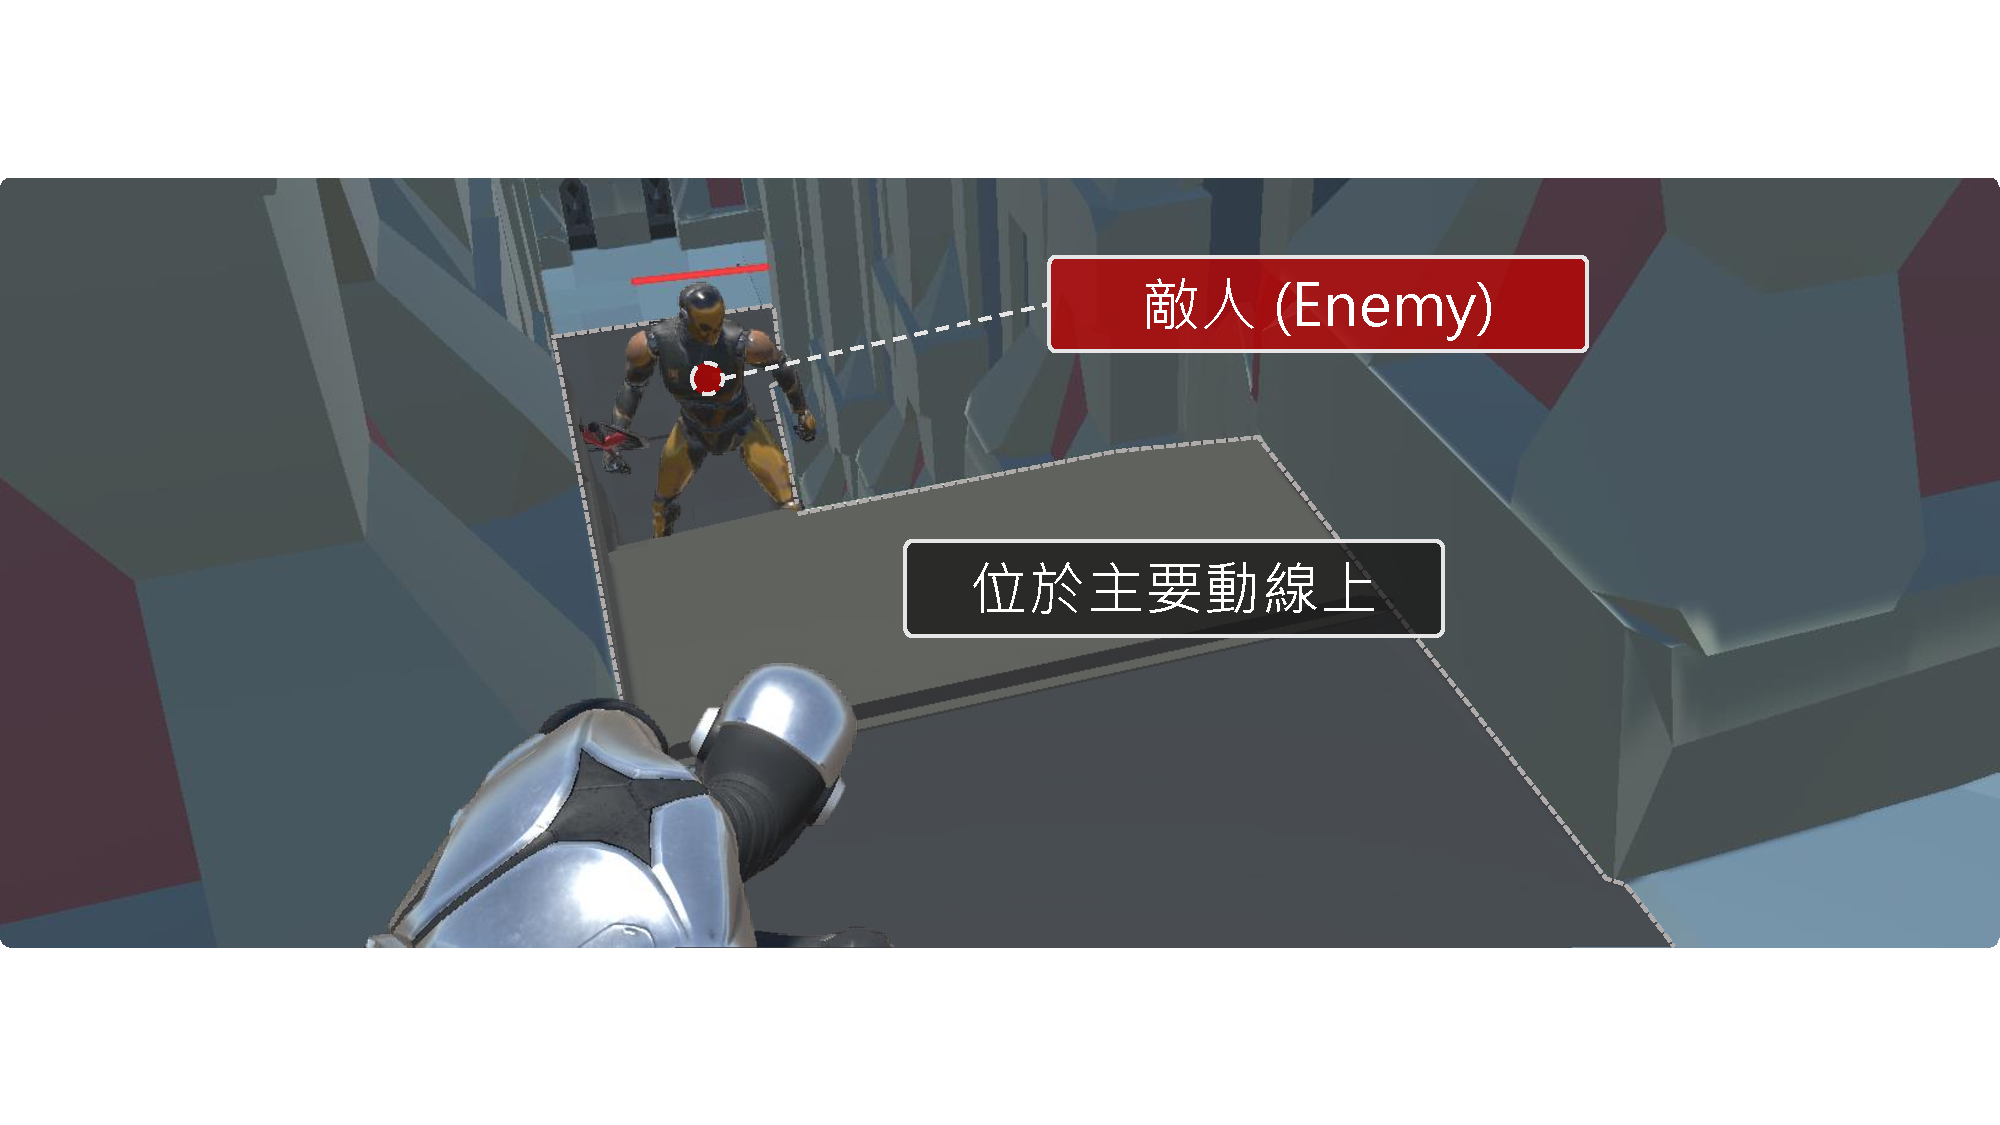
\includegraphics[width=1.0\textwidth]{figures/fitnesses-block-gameplay.pdf}
    \caption{阻擋點指標的遊戲體現情形}
    \label{fig:fitnesses-block-gameplay}
  \end{center}
\end{figure}

% \subsubsection{攔截點 (Intercept)}
% \label{sssec:method-segments-fitnesses-intercept}

% 方程式~\ref{eq:fitnesses-intercept} 為攔截點的適應性函數。與阻擋點近似,但敵人會避免被配置在空間動線上,為求快速追擊玩家為目的,將圍繞在空間動線附近。各敵人 ($E_{i}$) 越接近空間動線各點 ($MP_{j}$) 時影響愈大,且動線權重 ($mp_{j}$) 亦會影響加權程度。圖~\ref{fig:fitnesses-intercept-gameplay} 為攔截點指標的實際遊玩情形,草綠色區塊為系統計算出的空間動線的瓦磚,敵人將會被設置於動線周圍快速地攔截玩家。

% \begin{equation}
%     \label{eq:fitnesses-intercept}
%     f_{itc} = \sum_{i=1}^{M} \sum_{j=1}^{N} \Big( \frac{1}{dist(E_{i}, MP_{j})} \times mp_{j} \Big), 
%     E_{i} \neq MP_{j}
% \end{equation}

% \begin{figure}[!htb]
%   \begin{center}
%     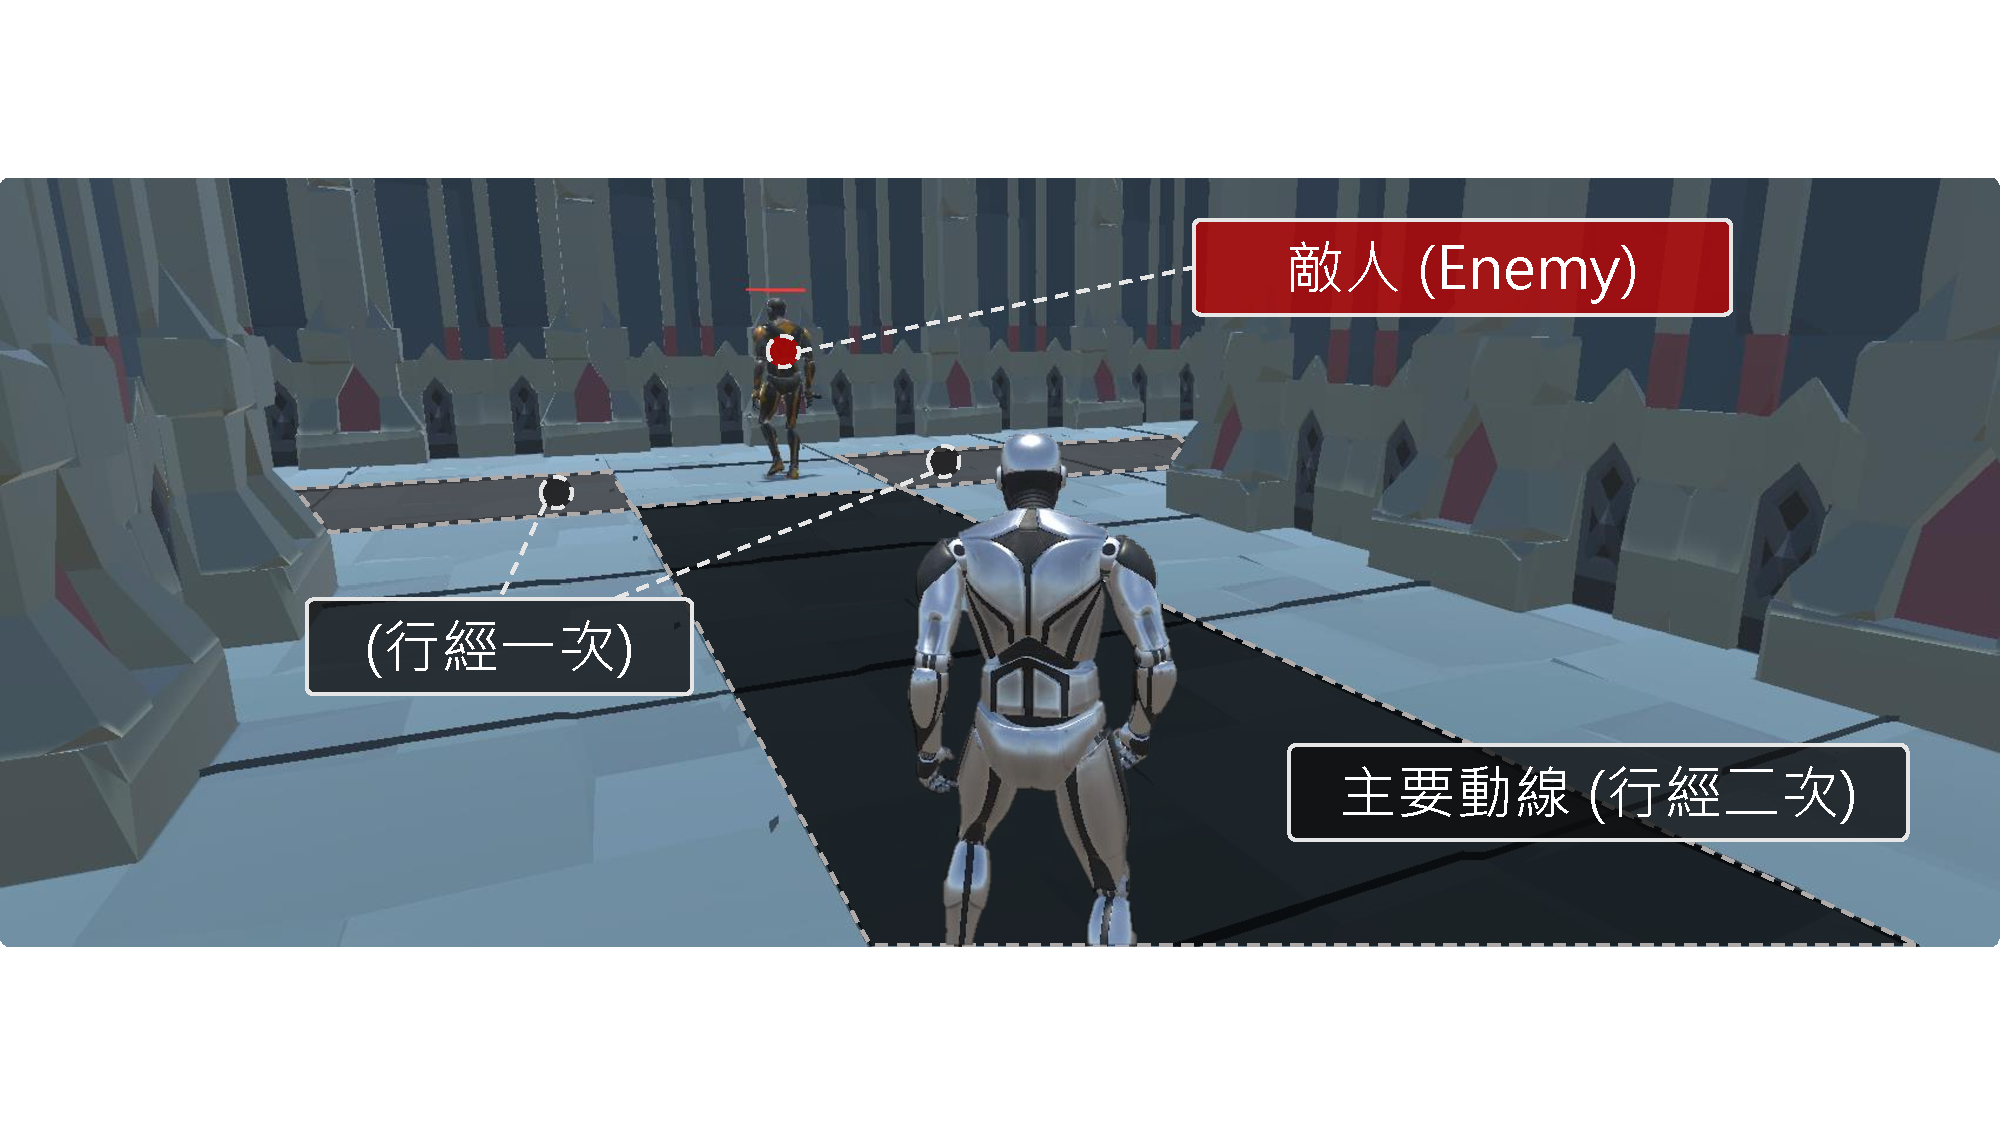
\includegraphics[width=1.0\textwidth]{figures/fitnesses-intercept-gameplay.pdf}
%     \caption{攔截點指標的遊戲體現情形}
%     \label{fig:fitnesses-intercept-gameplay}
%   \end{center}
% \end{figure}

\subsubsection{巡邏點 (Patrol)}
\label{sssec:method-segments-fitnesses-patrol}

方程式~\ref{eq:fitnesses-patrol} 為巡邏點的適應性函數。確保敵人擁有足夠的空間能夠進行移動,使其進行巡邏行為。$f_{ptl}$ 為 $M$ 個敵人 ($E_{i}$) 其方圓半徑 ($r$) 內相鄰可行走瓦磚之數量總合,計算各個可行走瓦磚 ($P_{j}$) 與敵人的直線距離,若距離小於或等於 $r$ 則值為 $1$,反之為 $0$。於本次實驗中,將採用 $r=3$ 作為實驗範例,該數值可由遊戲設計師決定。圖~\ref{fig:fitnesses-patrol-gameplay} 為巡邏點指標的實際遊玩情形,水藍色區塊為系統計算出的相鄰可走瓦磚,敵人會在此區域內執行巡邏的。

\begin{equation}
    \label{eq:fitnesses-patrol}
    f_{ptl} = \sum_{i=1}^{M} neighbor(E_i, r)
\end{equation}
\begin{gather*}
    neighbor(Obj, r) = \sum_{j=1}^{N} isNeighbor(Obj, P_{j}, r)
      \begin{cases}
        1, & \mbox{if } dist(Obj, P_{j}) \leq r \\
        0, & \mbox{if } dist(Obj, P_{j}) > r
      \end{cases}
\end{gather*}

\begin{figure}[!htb]
  \begin{center}
    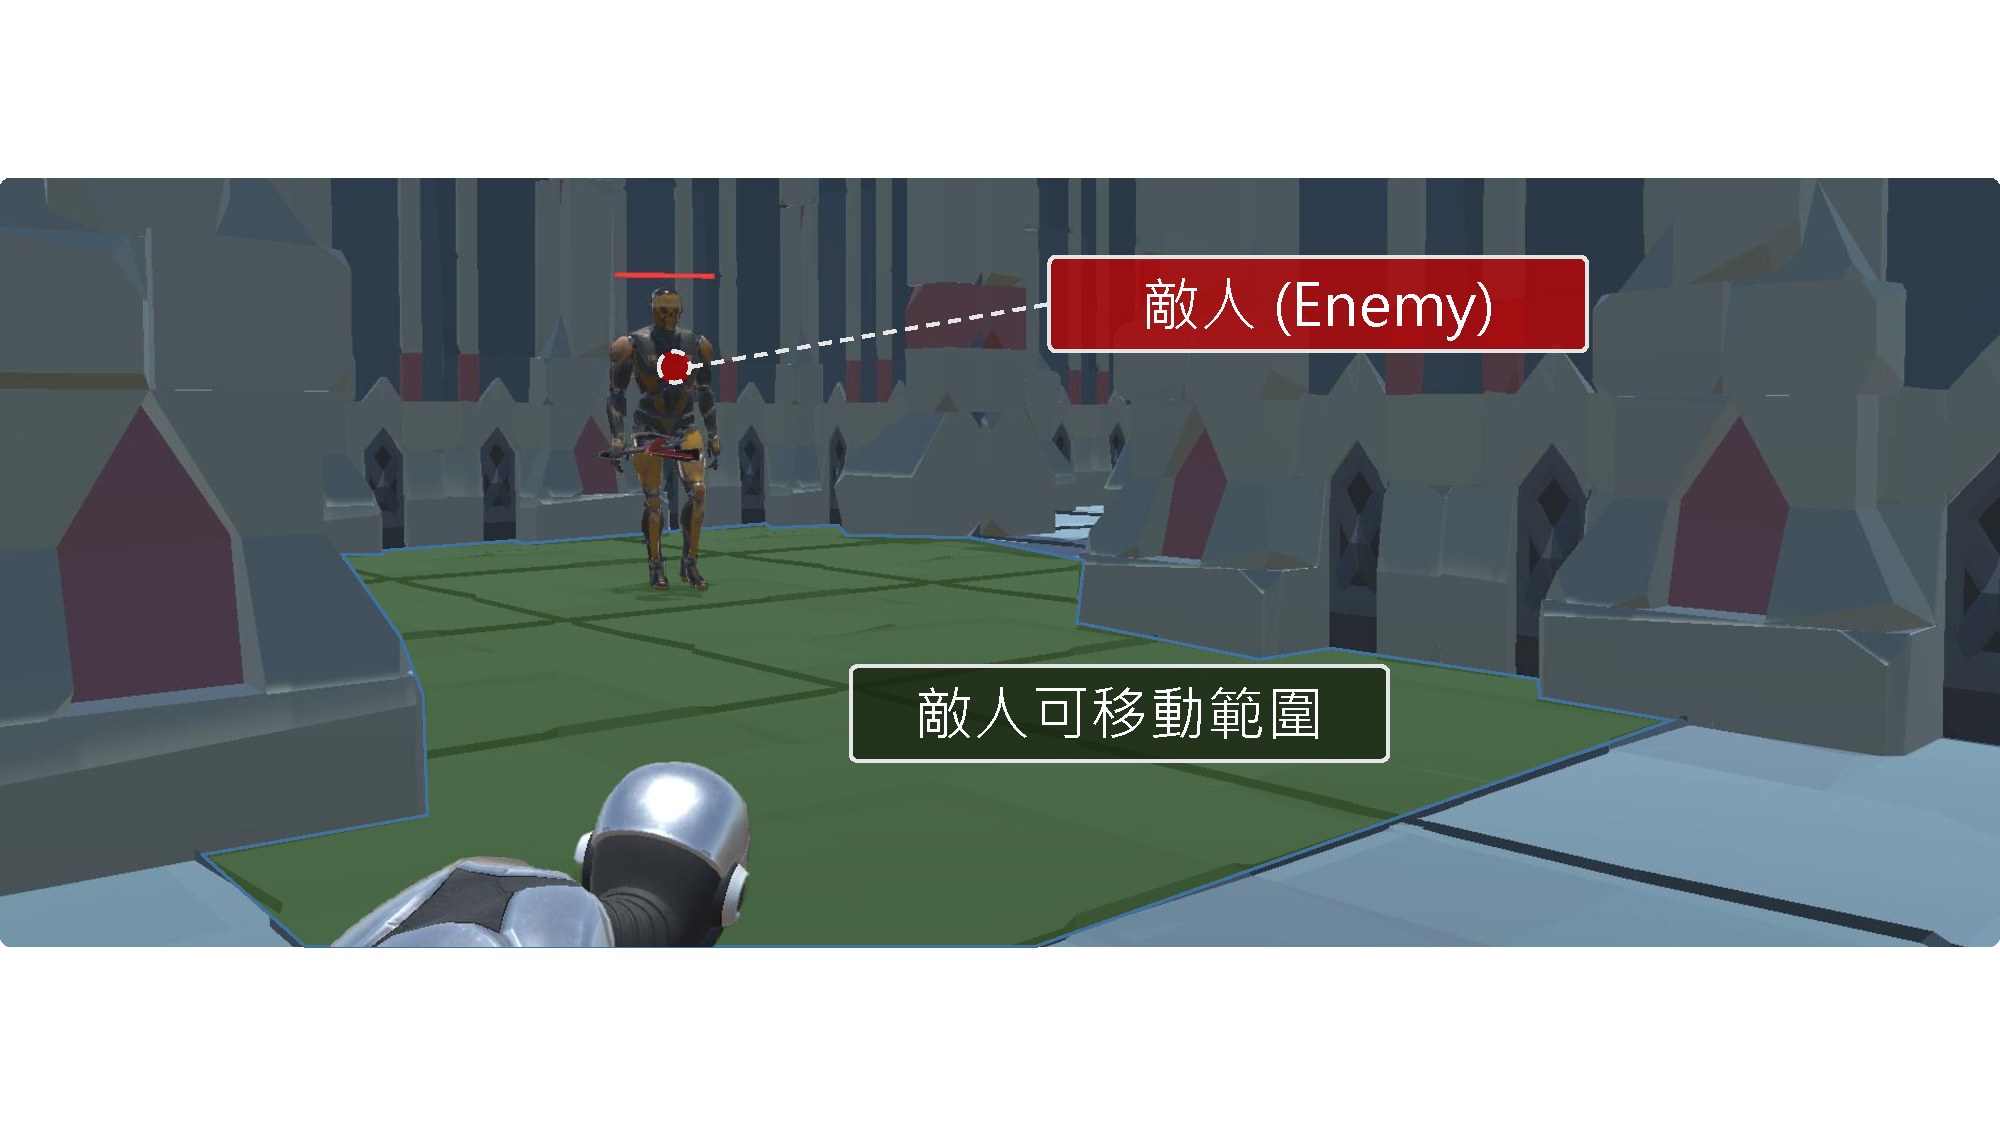
\includegraphics[width=1.0\textwidth]{figures/fitnesses-patrol-gameplay.pdf}
    \caption{巡邏點指標的遊戲體現情形}
    \label{fig:fitnesses-patrol-gameplay}
  \end{center}
\end{figure}

% \subsubsection{支援點 (Support)}
% \label{sssec:method-segments-fitnesses-support}

% 敵人 ($E_{i}$, $E_{j}$) 之間擁有一定程度的護援關係,當敵人彼此的距離愈低其影響程度越大,同時該敵人 ($E_{i}$) 必須遠離動線 ($MP_{k}$)。

% \begin{equation}
% f_{sup}=\frac{1}{N} \sum_{i=1}^{N} \bigg( \frac{1}{N} \sum_{\substack{j=1 \\ j \neq i}}^{N} \frac{1}{dist(E_{i}, E_{j})} + \frac{1}{M} \sum_{k=1}^{M} \frac{1}{dist(E_{i}, MP_{k})} \bigg)
% \end{equation}

% \begin{figure}[!htb]
%   \begin{center}
%     
\includegraphics[width=1.0\textwidth]{figures/under_construction.png}
%     \caption{支援點指標的遊戲體現情形}
%     \label{fig:fitnesses-support-gameplay}
%   \end{center}
% \end{figure}

% \subsubsection{陷阱點 (Trapped)}
% \label{sssec:method-segments-fitnesses-trapped}

% \begin{equation}
%     f_{trp} = 
% \end{equation}

% \subsubsection{死角點 (Neglected)}
% \label{sssec:method-segments-fitnesses-neglected}

% 由於房與房之間的牆壁阻隔,使得敵人能夠埋伏於入口附近之死角處,出奇不意地對玩家展開攻擊。為了體現出這種現象,我們將敵人 ($E_{i}$) 與空間動線上各點 ($MP_{i}$),兩端點連線之對角線所構成的立方體,立方體所涵蓋各座標點 ($N_{j}$) 至該對角線的距離為 $d_{k}$,隨著距離增加影響程度會衰減;$vis_{k}$ 為該點的可視情形,若有不可視的座標存在便會提高適應值。隨著動線的順序演進,影響程度逐漸衰減。

% \begin{equation}
%     Under construction
% \end{equation}


% \subsubsection{至高點 (Dominated)}
% \label{sssec:method-segments-fitnesses-dominated}

% 當玩家可能所在動線上之位置 ($MP_{j}$) 與敵人的位置 ($E_{i}$) 具有高低差時,敵人便適合採取遠程攻擊;為了提供玩家思考對付遠程敵人的緩衝時間,將敵人配置於動線末端附近是較好的選擇,$j$ 隨著動線的順序演進,影響程度逐漸增幅。

% \begin{equation}
% f_{dom}=\sum_{i=1}^{N} \sum_{j=1}^{M} \Big( \frac{1}{dist\big(E_{i}, MP_{j}\big)} \times mp_{j} \times j \times high(E_{i}, MP_{j}) \Big)
% \end{equation}


\subsection{制衡取向的適應性函數}
\label{ssec:method-segments-balancefitness}

於~\ref{ssec:method-segments-fitnesses} 小節所提及的適應性函數中,函數皆有著一項共通點,便是隨著符合遊玩特徵的物件數量與適應值呈現顯著正相關,隨著演化代數的提升至終導致房間容器充斥著大量的遊戲物件。然而這樣的遊玩體驗在絕大多數都是不可行的,因此需要針對現有適應性函數所衍生出的特性,設計抑制其得分隨著數量級的成長。

方程式~\ref{eq:fitnesses-density} 控制該房間容器出現的遊戲物件總數。房間容器的物件總數上限為 $M$、下限為 $N$,若遊戲物件總數 $O$ 於數量範圍內可得 $1$ 分,反之得 $0$ 分,本適應性函數的權重固定為其餘權重絕對值之合,最小為 $1$,$w_{dst} = max(1, \sum_{i=1}^{amount} \lvert w_{i}\rvert)$。

\begin{equation}
    \label{eq:fitnesses-density}
    f_{dst} = \begin{cases}
                  1, & \mbox{if } N \leq O \leq M \\
                  0, & \mbox{if } O<N \text{ or } O>M
              \end{cases}
\end{equation}

% \subsection{負數權重的適應性函數}
% \label{ssec:method-segments-minusscores}

% 在~\ref{sssec:method-segments-fitnesses-guard} 守衛點指標的設計中,當權重為正數時能夠體現出「需要被保護的物件,其周圍分配敵方單位進行守衛」的遊玩特徵,且在多個物件的情形下儘可能平均分配敵方單位;反之,負數權重便會體現出「數量愈不平均的守衛情形」。緣故為設計守衛點指標時,並無針對寶箱的數量進行控管而導致。

\subsection{多項適應性函數合併}
\label{ssec:method-segments-multiobjectives}

在設計適應性函數初期,為求多個適應性函數相互牽制,進而求得限制條件的最佳解。而初期函數會力求場上所有的敵人必須盡可能符合各項指標。舉例來說,在某一房間容器的設定中,我們將守衛點、阻擋點的權重調整至 $1$,其餘指標將不採計得分即不調整權重,倘若場面上存在著敵人 A 與 敵人 B,他們會同時被設置在動線上且一定距離內會有作為守護對象的寶箱物件。但對於遊戲設計師在某些情形下,敵人 A 與敵人 B 僅需要分別符合守衛點、阻擋點指標,才是理想中的遊玩特徵。因此,我們定義「首次出現相關遊玩特徵的得分幅度最顯著」,並依照出現數量逐漸下降成長幅度且逼近於 $1$,呈現近似於對數函數圖形的曲線,因此上述兩種情形都有機會成為演化過程中的最適解。取代原先的線性成長關係,進行數值的標準化,強制將值域規範至 $[0, 1]$ 以求最後適應性函數加權總分時,不偏袒任何適應性函數以達到公平基準。

方程式~\ref{eq:fitnesses-all} 中定義房間容器(個體)的品質,參考 Abdullah Konak 提出的~\textit{Weighted sum approaches}~\cite{konak2006multi} 並予以改良。採計共 $M$ 種適應性函數,第 $i$ 項適應值為 $f_{i}$ 並經過標準化 $Normalized(f_{i}) = [0, 1]$,依照各函數得分與其權重值 $w_{i} = [-1, 1]$ 加權後加總得到 $f_{all}$。而標準化由個體分數 $f_{i}$ 除以該世代最高得分 $f_{i}\cdot max$ 開 $c$ 次方根。

\begin{equation}
    \label{eq:fitnesses-all}
    f_{all} = \sum_{i=1}^{M} (Normalized(f_{i}) \times w_{i})
\end{equation}
\begin{gather*}
    Normalized(f_{i}) = (\frac{f_{i}}{f_{i}\cdot max})^{\frac{1}{c}}
\end{gather*}

圖~\ref{fig:fitnesses-normalized} 中顯示了方程式~\ref{eq:fitnesses-all} 依照不同的自然數常數 $c$ 進行適應值的標準化。在此圖~\ref{fig:fitnesses-normalized} 中定義 $x\cdot max = 10$ 方便後續的解釋工作。$y_{1}$ 為原始分數除以原始分數最大值之標準化,初期的成長幅度為 $x_{12} - x_{11} = 0.1000$,隨著原始分數的增加並不影響後續的成長幅度 $x_{14} - x_{13} = 0.1000$。為了要體現出前述之定義「首次出現相關遊玩特徵的得分幅度最顯著」的現象,我們對 $y_{1}$ 的數值再進行開 $c$ 次方根,分別以 $c = 2$、$c = 3$ 與 $c = 4$ 得到 $y_{2}$、$y_{3}$ 與 $y_{4}$ 三種線性方程式,其中 $y_{2}$ 的初期成長幅度為 $x_{22} - x_{21} = 0.1310$ 高於 $y_{1}$ 同期的成長幅度,到了後期的成長幅度為 $x_{24} - x_{23} = 0.0847$,逐漸衰減同時已低於 $y_{1}$ 同期的成長幅度,然而這樣的現象隨著常數 $c$ 上升對於分數初期的成長幅度愈大、後期的成長幅度愈小。

\begin{figure}[!htb]
  \begin{center}
    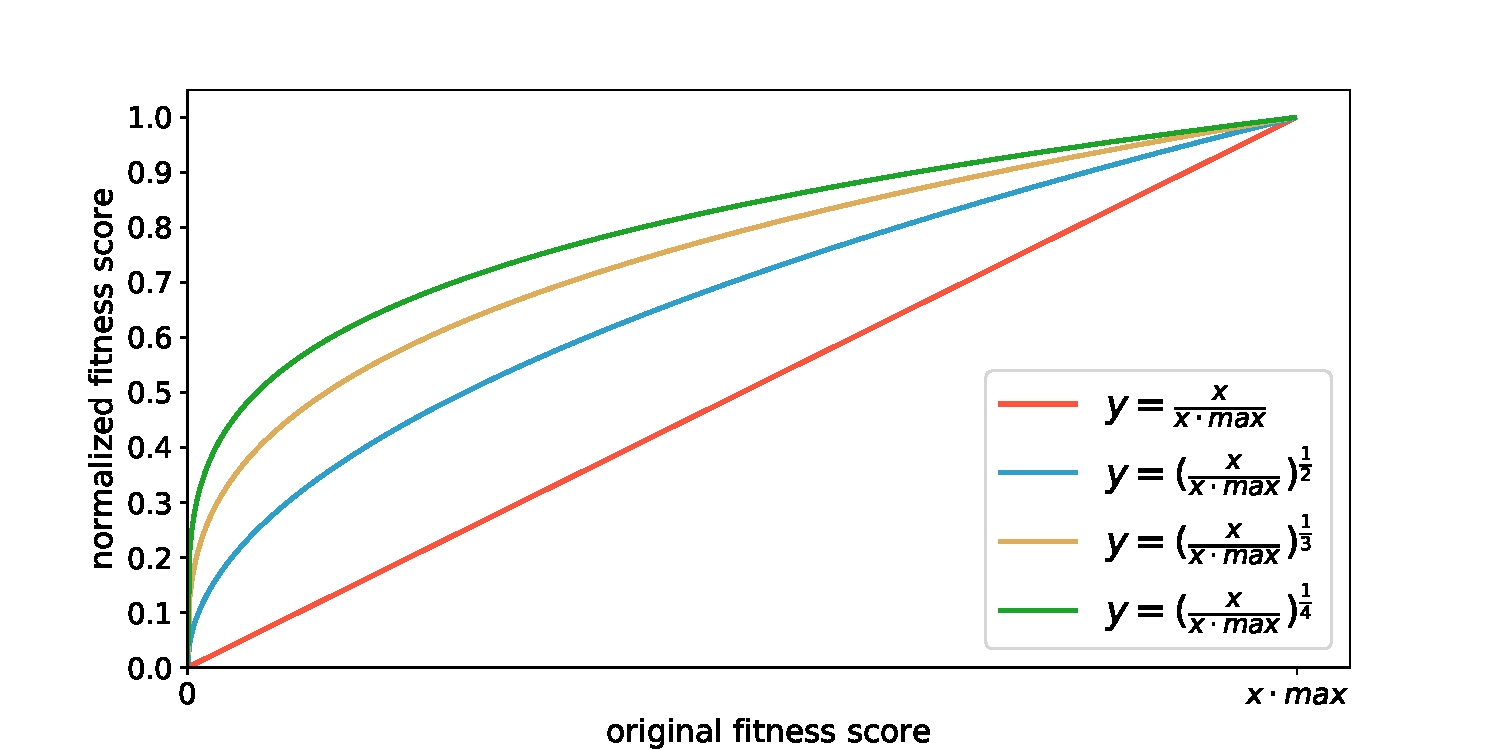
\includegraphics[width=1.0\textwidth]{figures/fitnesses-normalized.pdf}
    \caption{適應值進行標準化}
    \label{fig:fitnesses-normalized}
  \end{center}
\end{figure}

舉例來說,承接圖~\ref{fig:fitnesses-normalized} 的原始標準化線性方程式如 $y_{1}$,並假設一個體 $a$ 有守衛點適應值 $y_{guard_{1a}} = 0.2$ 與阻擋點適應值 $y_{block_{1a}} = 0.4$;另一個體 $b$ 有守衛點適應值 $y_{guard_{1b}} = 0.0$ 與阻擋點適應值 $y_{block_{1b}} = 0.7$。在上述情形中,個體 $a$ 的總適應值為 $0.6$、個體 $b$ 的總適應值為 $0.7$,被列為最佳個體的會是個體 $b$。但綜觀來看個體 $a$ 的各個遊玩指標均衡發展,個體 $a$ 應當是比個體 $b$ 更能夠體現出複合型的遊玩指標。經過調整後的標準化線性方程式 $y_{2}$,個體 $a$ 的總適應值為 $y_{guard_{2a}} + y_{block_{2a}} = 0.4472 + 0.6324 = 1.0796$、個體 $b$ 的總適應值為 $y_{guard_{2b}} + y_{block_{2b}} = 0.0000 + 0.8366 = 0.8366$,此時能夠體現出複合型遊玩指標的個體 $a$ 將會被視為是更優良的個體。

\subsection{套用物件演化機制的房間容器}
\label{ssec:method-segments-appliedonvolumes}

綜合上述小節,不同房間容器類型會有對應的戰略配置。~\ref{ssec:method-spacepieces-types} 小節所介紹的房間容器外,在本小節追加了戰鬥通道的房間容器,與前章節提及之通道不同處,在戰鬥通道中玩家恐會遭遇敵方單位。戰鬥通道的格局是經過特殊設計的,敵方單位能夠依照不同房型格局進行對應的戰鬥策略,見圖~\ref{fig:roomtype-mainpath-extend}。因此依照房間容器類型設置不同的適應性函數權重,逐一定義各自的適應性函數權重值。

\begin{figure}[!htb]
  \begin{center}
    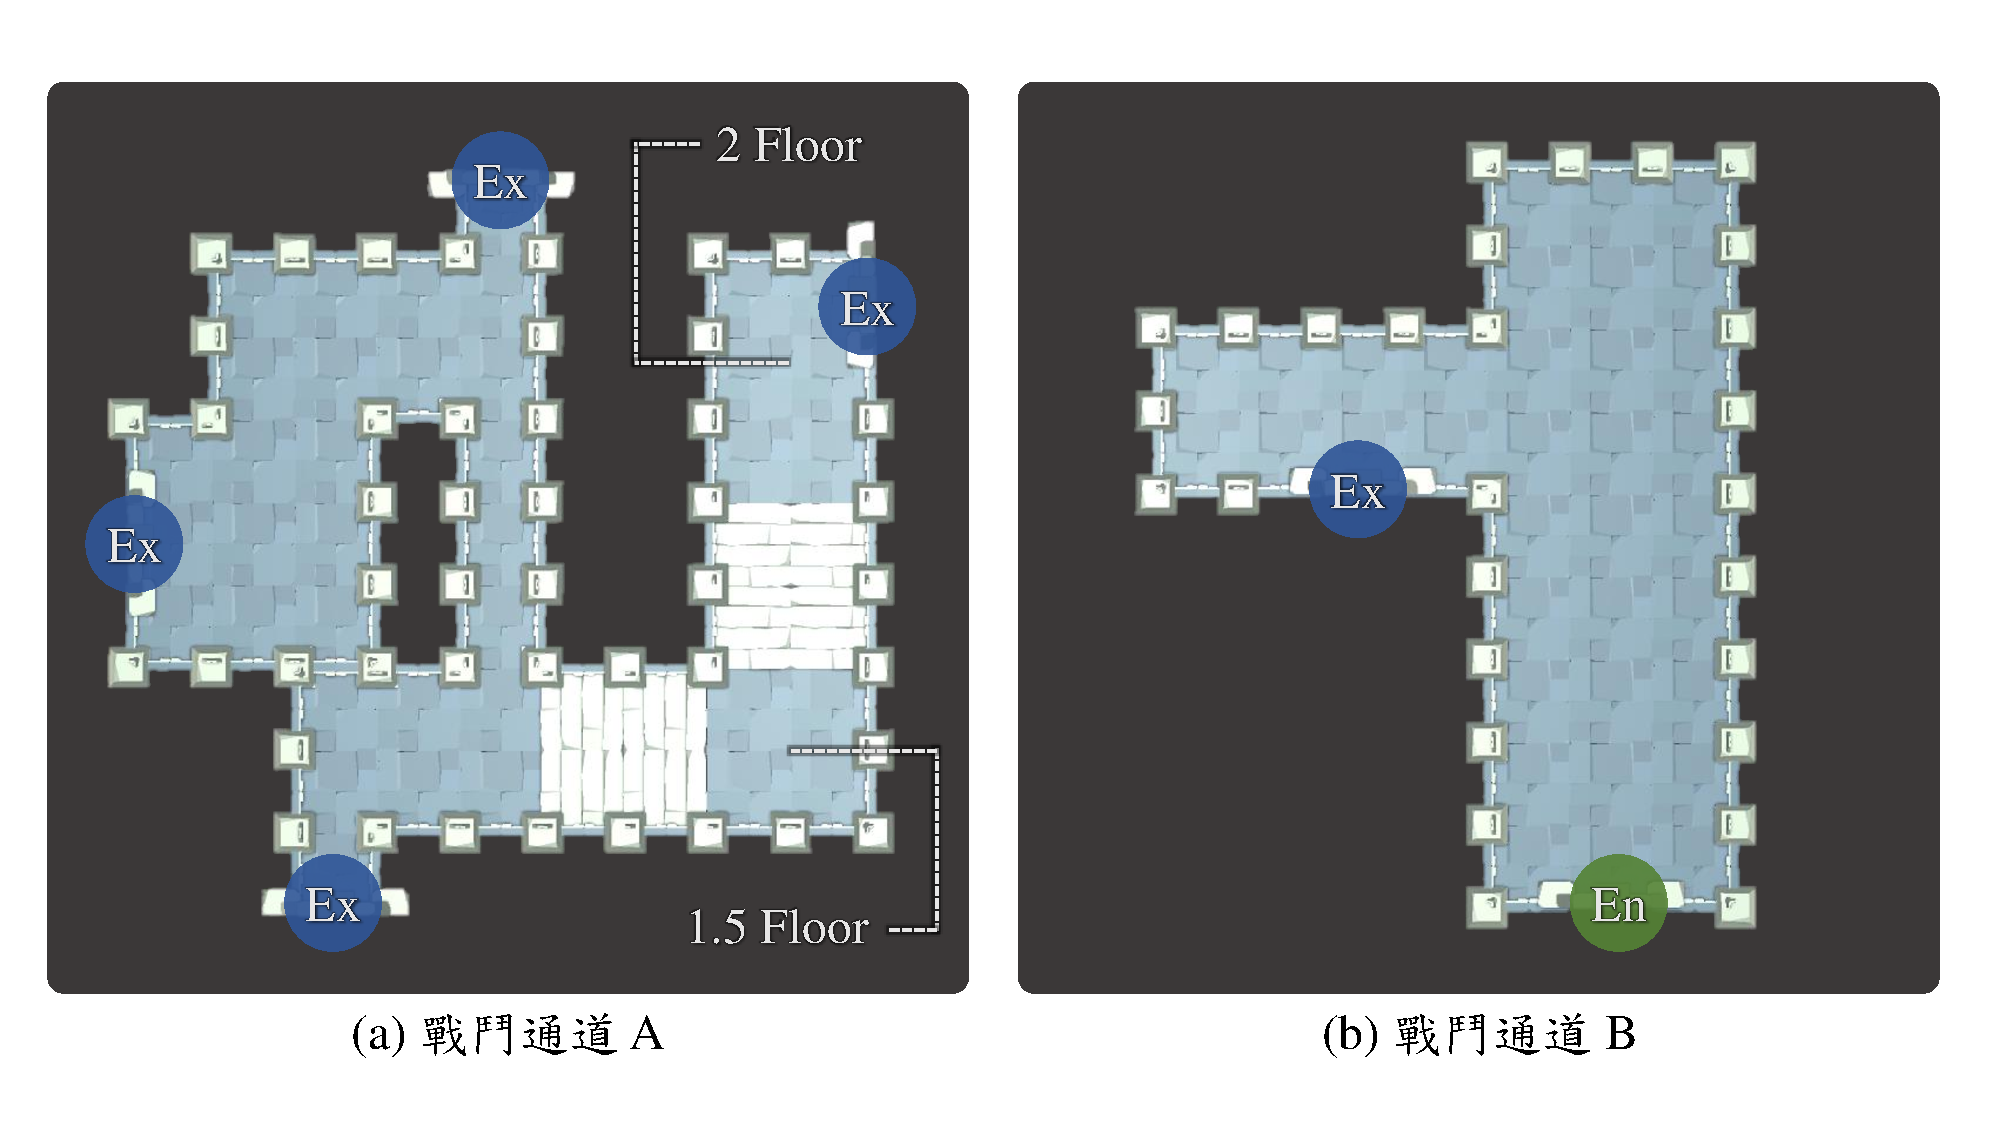
\includegraphics[width=1.0\textwidth]{figures/roomtype-mainpath-extend.pdf}
    \caption{擴充房間容器,戰鬥通道的房間容器結構}
    \label{fig:roomtype-mainpath-extend}
  \end{center}
\end{figure}

\subsubsection{寶藏房}
\label{sssec:method-segments-appliedonvolumes-treasure}

寶藏房的端點識別物僅只有一個入口端點,便不存在空間動線,與空間動線相關的適應性函數不予採計。圖~\ref{fig:applied-ga-on-volume-treasure} 是寶藏房的演化結果,圖~\ref{fig:applied-ga-on-volume-treasure} i-iii 的演化結果呈現出,敵人與寶箱物件彼此間的距離關係鄰近,敵人物件便能夠對相鄰寶箱物件進行守衛動作。

\begin{itemize}
  \setlength\itemsep{-0.5em}
  \item 守衛點權重: $1.00$
  \item 遊戲物件數量限制: $[3, 5]$
\end{itemize}

\begin{figure}[H]
  \begin{center}
    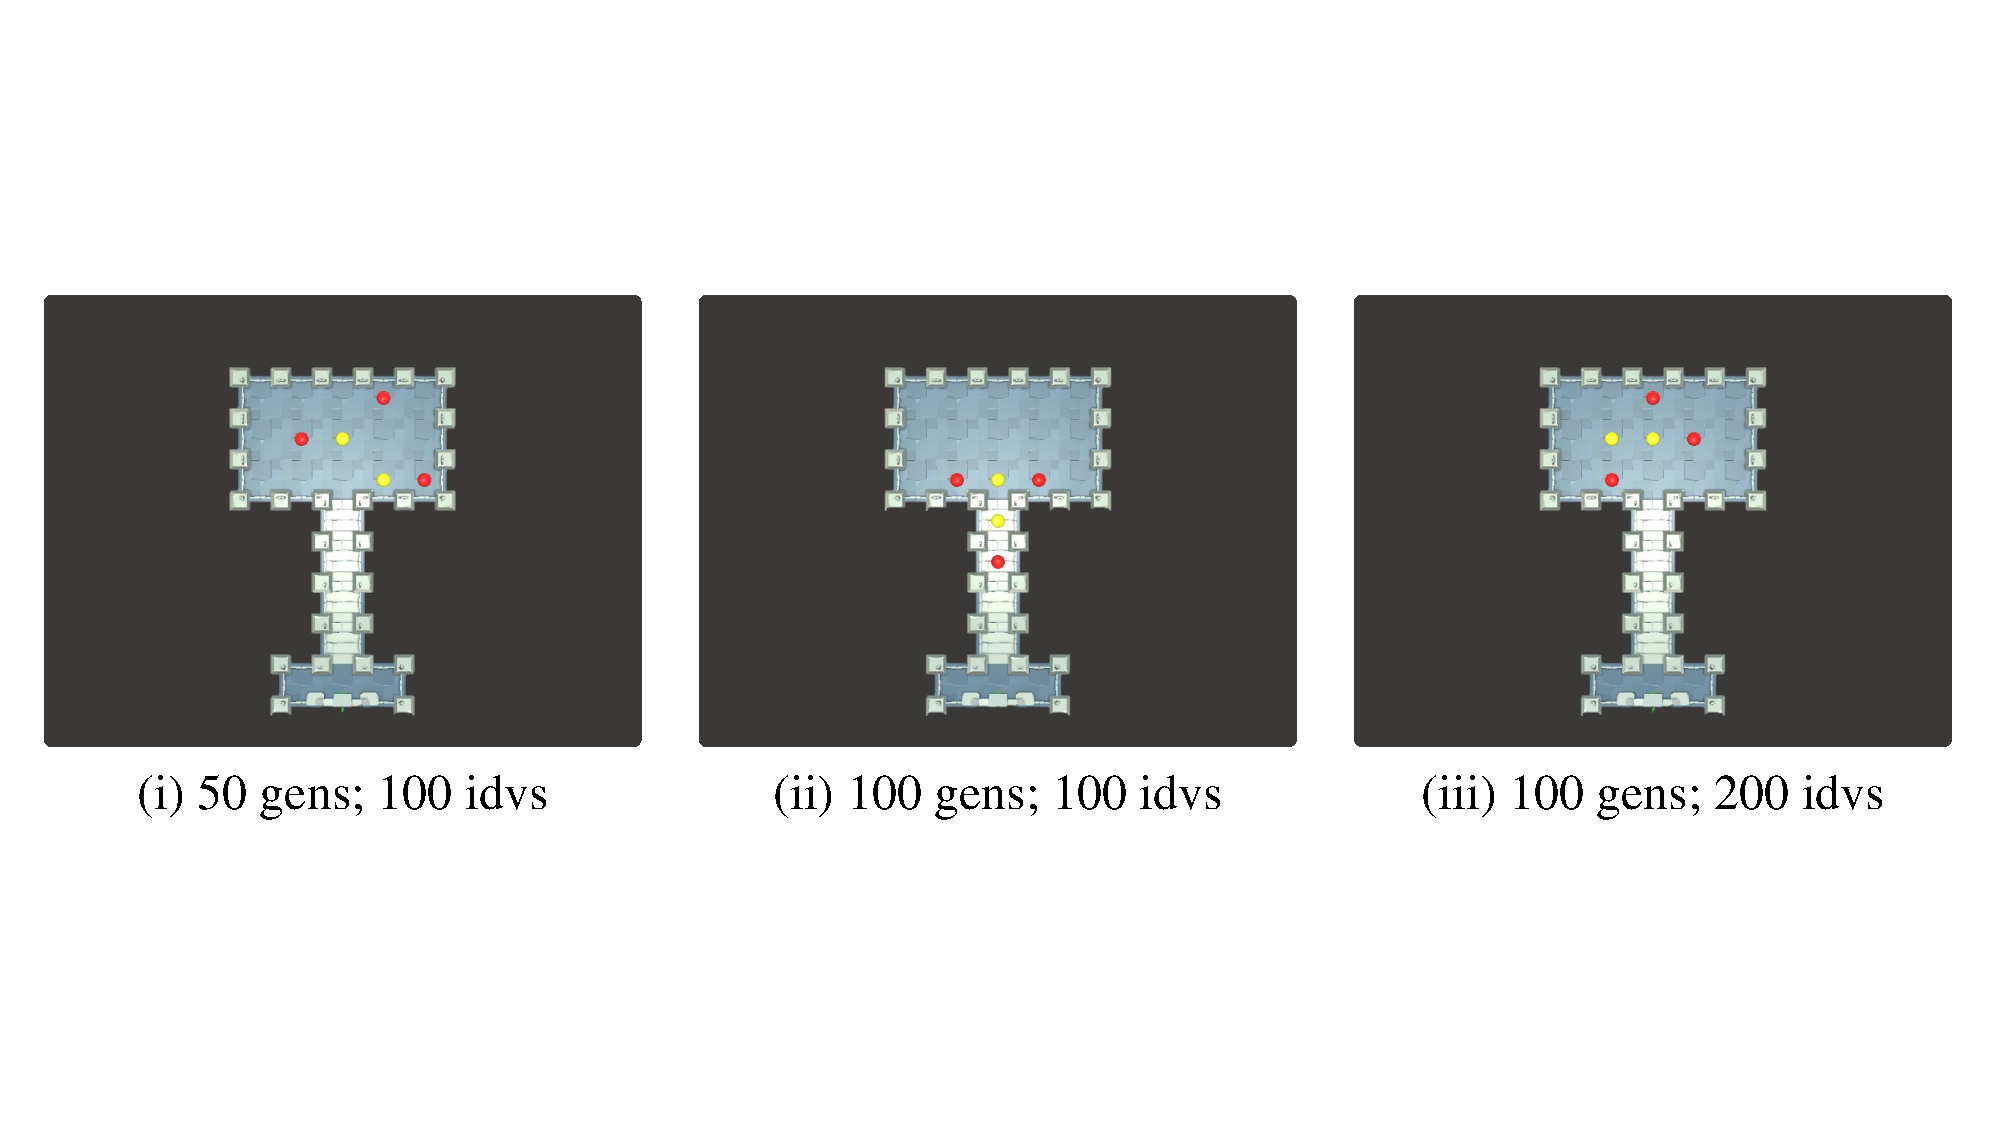
\includegraphics[width=1.0\textwidth]{figures/applied-ga-on-volume-treasure.pdf}
    \caption{寶藏房的遊戲物件佈局演化示意} 
    \label{fig:applied-ga-on-volume-treasure}
  \end{center}
\end{figure}

\subsubsection{戰鬥通道(狹路驅逐)}
\label{sssec:method-segments-appliedonvolumes-battlepath-narrow}

戰鬥通道(狹路驅逐)無入口端點、有四個出口端點。在此房間容器中,西方出口為一廣場;東方出口位於二樓;在北方出口與南方出口之間有一狹長的通道,是連接各個出口的必經道路。

在此房間容器的佈局預期讓玩家體驗到重要幹道被敵人所盤據,玩家必須在該幹道上與敵人發生衝突方可通過,便將阻擋點指標之權重設為 $1.00$,並以南方出口作為入口。且在寬廣地區亦有機會設置敵人進行巡邏監視,便將巡邏點指標之權重設為 $0.75$。圖~\ref{fig:applied-ga-on-volume-battlepath-narrow-i} 是戰鬥通道(狹路驅逐)的演化結果,並以南方出口作為入口,圖~\ref{fig:applied-ga-on-volume-battlepath-narrow-i} i-iii 能觀察到,並非所有的點都坐落在高權重的空間動線座標上,因為巡邏點指標的關係,將敵人物件放置於他處也能獲得相當不錯的部分適應值。

\begin{itemize}
  \setlength\itemsep{-0.5em}
  \item 阻擋點權重: $1.00$
  \item 巡邏點權重: $0.75$
  \item 遊戲物件數量限制: $[4, 5]$
\end{itemize}

\begin{figure}[H]
  \begin{center}
    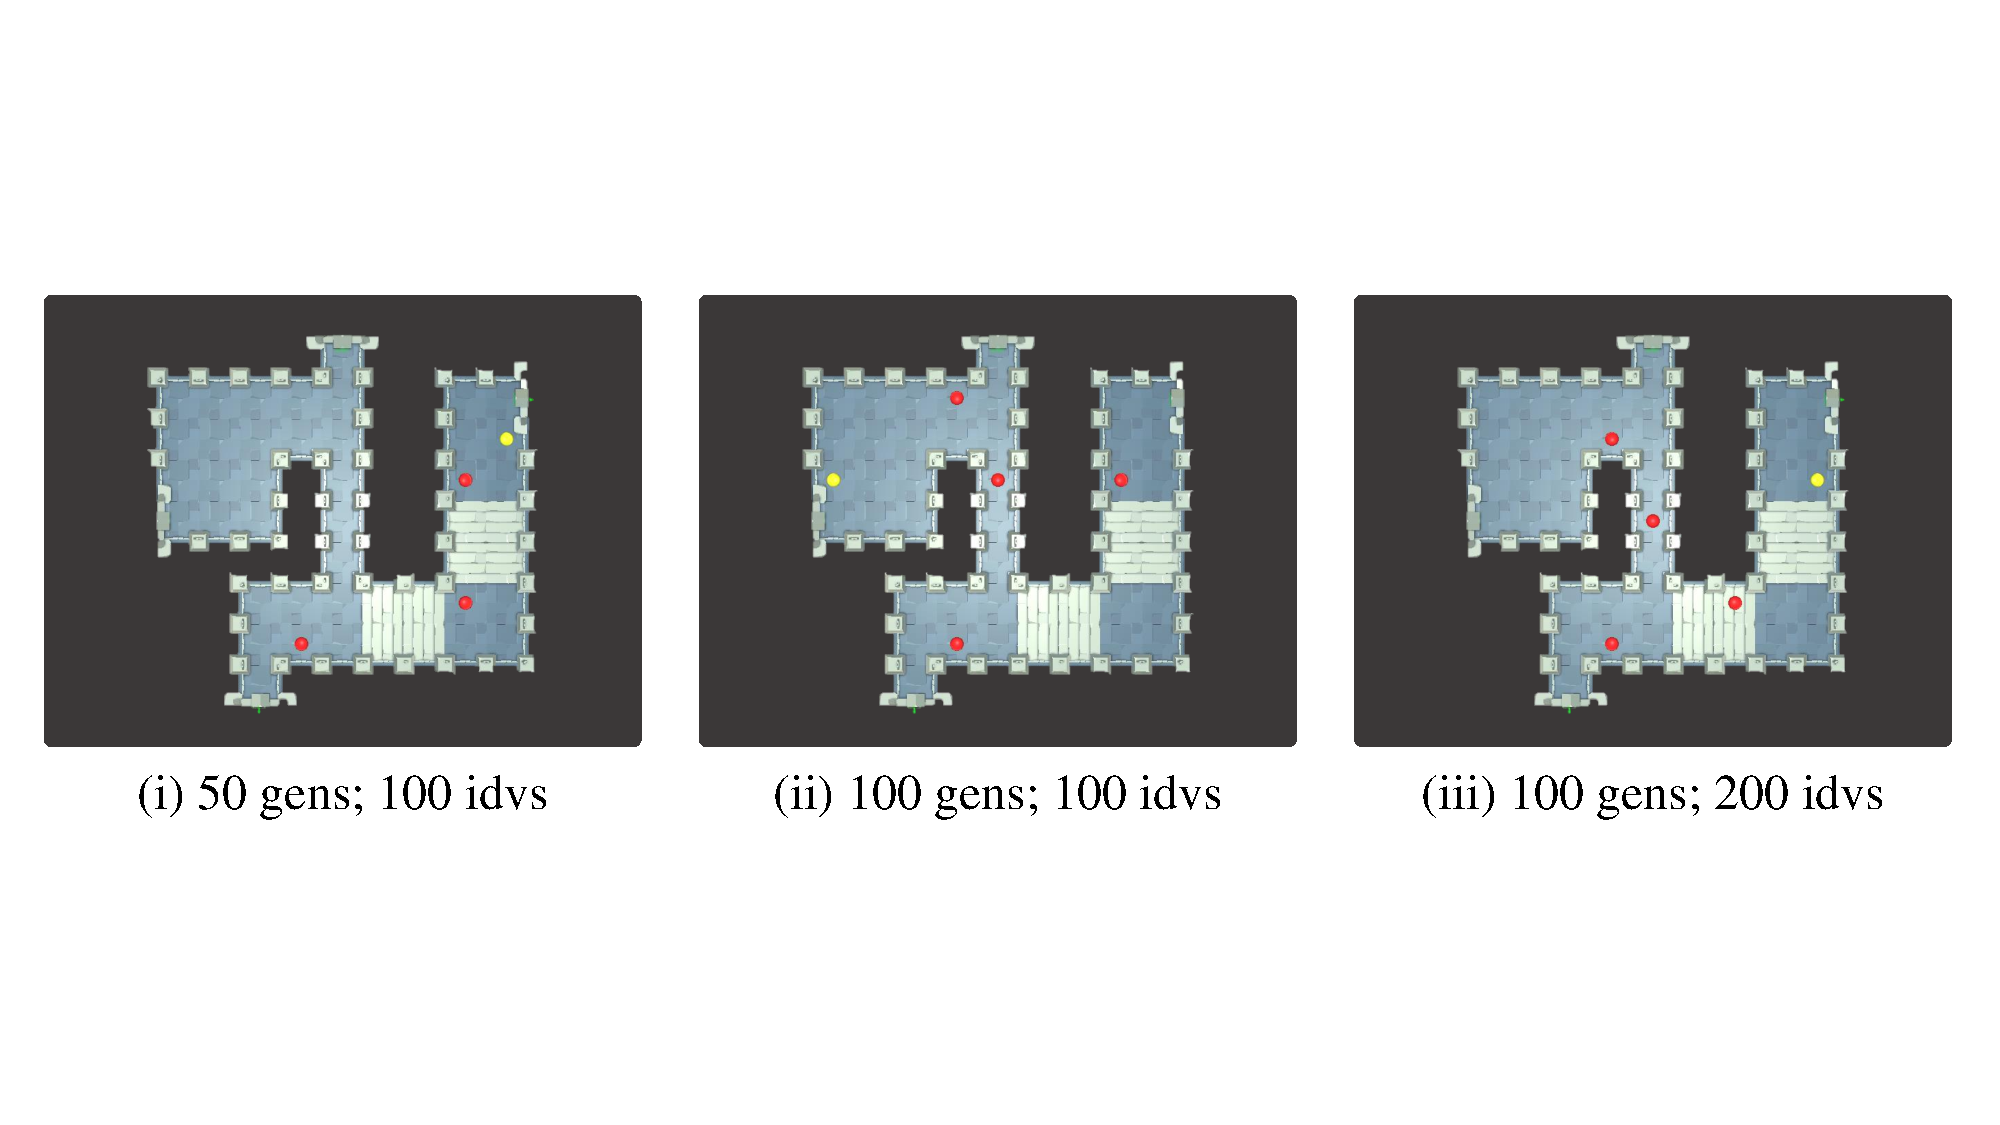
\includegraphics[width=1.0\textwidth]{figures/applied-ga-on-volume-battlepath-narrow-i.pdf}
    \caption{狹路驅逐情境 II 的遊戲物件佈局演化示意} 
    \label{fig:applied-ga-on-volume-battlepath-narrow-i}
  \end{center}
\end{figure}

\subsubsection{戰鬥通道(鎮守要道)}
\label{sssec:method-segments-appliedonvolumes-battlepath-trunk}

戰鬥通道(鎮守要道)有一個入口端點及一個出口端點,在此房間容器的佈局與狹路驅逐近似,但敵人將專注於戰鬥陣行,將不會存在寶箱。圖~\ref{fig:applied-ga-on-volume-battlepath-trunk} 是戰鬥通道(鎮守要道)的演化結果,圖~\ref{fig:applied-ga-on-volume-battlepath-trunk} i-iii 能夠觀察到演化結果中都不再存在寶箱物件。

\begin{itemize}
  \setlength\itemsep{-0.5em}
  \item 阻擋點權重: $1.00$
  \item 巡邏點權重: $0.50$
  \item 守衛點權重: $-1.00$
  \item 遊戲物件數量限制: $[3, 5]$
\end{itemize}

\begin{figure}[H]
  \begin{center}
    \includegraphics[width=1.0\textwidth]{figures/applied-ga-on-volume-battlepath-trunk.pdf}
    \caption{鎮守要道情境的遊戲物件佈局演化示意} 
    \label{fig:applied-ga-on-volume-battlepath-trunk}
  \end{center}
\end{figure}

\subsubsection{其餘房間容器}
\label{sssec:method-segments-appliedonvolumes-others}

其餘未被定義的房型,像是入口、出口、一般通道 ... 等,因設計需求將不配置任何遊戲物件,即不參與相關的演化流程。圖~\ref{fig:applied-ga-on-volume-all} 略過不需要進行演化的房間容器,並針對有設置遊玩特徵指標的房間容器進行演化。

\begin{figure}[!htb]
  \begin{center}
    \includegraphics[width=1.0\textwidth]{figures/applied-ga-on-volume-all.png}
    \caption{將關卡中全部房間容器進行遊戲物件的佈局演化} 
    \label{fig:applied-ga-on-volume-all}
  \end{center}
\end{figure}

\section{方法彙整與總結}
\label{sec:method-summary}

圖~\ref{fig:completed-framework} 將上述所提及之方法彙整至其中,共計三大項目。第~\ref{sec:method-missiongrammars} 節介紹了「任務語法」,讓關卡設計師能透過抽象宏觀的概念,藉由直覺的圖形介面生成出任務圖,表達出遊玩流程的拓撲結構。第~\ref{sec:method-spacepieces} 節介紹了「空間建構」,從建構房間容器的最小體素單位至端點識別物,並且透過改寫系統將任務圖轉換至遊戲空間。第 ~\ref{sec:method-segments} 節介紹了「地圖片段演化方法」,將房間容器依照不同的戰略要素,給予不同遊玩特徵指標的權重,最後利用基因演算法逐步演化得到遊戲物件的關卡最適佈局。

\begin{landscape}
  \begin{figure}[!htb]
    \begin{center}
      \includegraphics[width=1.0\linewidth]{figures/completed-framework.pdf}
      \caption{本論文提出之方法,完整框架示意圖} 
      \label{fig:completed-framework}
    \end{center}
  \end{figure}
\end{landscape}